\documentclass{article}
\usepackage{verbatim, seqsplit, graphicx}
\usepackage[total={7in,9in}]{geometry}

\begin{document}

\title{\Large Deep learning 2. Big homework 1}
\author{Alexey Slizkov}
\date{04.12.2023}
\maketitle

\vspace{25pt}

In this report, I present the results of training several Language Models (LLMs), gradually scaling them up. The vocabulary used consisted of 4096 tokens.

\section{General information}


\subsection*{11M parameters}

\subsubsection*{20 epochs | Final loss: 4.1032}

Sample text: \begin{verbatim}
\textbf{Once upon a time}, there was a little girl named Sheish feeling on the inside across.
One day, a burning animal was standing
\end{verbatim}...


\subsection*{32M parameters}

This model was trained on 3.8B tokens in total over 20 epochs (190M tokens per epoch).

\subsubsection*{20 epochs | Final loss: 2.1593}

Sample text: \begin{verbatim}
\textbf{Once upon a time}, there was a modest little boy named Tim. He loved to read books, even a big
book like Spot. One day, Tim asked his mom if he ever wanted a warm math. His mother said, "No,
Tim! You will make me strong, but you be careful not to be too strong to hurt his clothes."
Tim thought about this moment and said, "No, we are a good family. Your books is a good girl who
I want to be happy land with me and learn." His mom forgave him and they all played together.
When they got to the show, Tim gave it to his mom and dad to play. He said, "Wow, that's cool,
Mom! I can make a normal shirt for you." Tim felt very happy and dry. The barber became good
friends and Finn learned that the important help was the importance of others can change.
\end{verbatim}


\subsection*{114M parameters}

This model was trained on 3.4B tokens.

Sample text: \begin{verbatim}
\textbf{Once upon a time}, there was a little girl named Lily. Lily loved to follow her mommy in the photo.
One day, Lily was skipping when she saw a monkey running away fast. She was so curious, she ran
over towards it! The monkey was running past her and Lily laughed and clapped her hands.
Suddenly, Lily discovered a butterfly fluttering her path. She waved goodbye up and the monkey
ran away. Lily ran after the butterfly and went back to searching. She looked behind the mark
and saw a butterfly. She wished she had listened to her mommy. Suddenly, Lily heard a hide behind
a tree. She peeked behind the tree and saw the butterfly. She looked and saw that it was growing
in a tree. Lily was so delighted that she ran and sat down. But then, she accidentally dropped
her hand, and she fell down from the tree. She scraped all over the ground and saw her sneeze on
her face. From then on, Lily learned to be careful not to hurt animals.
\end{verbatim}


\subsection*{329M parameters}

This model was trained on 9.1B tokens in total (10x our whole dataset).
The total training time was 139 hours.

\subsubsection*{10 epochs | Final loss: 1.2583}

Sample text: \begin{verbatim}
\textbf{Once upon a time}, there was a little girl named Lily. She loved to skip and play in the park.
One day, she saw a big giant sitting on a bench. She was so excited and she skipped down
the bench to sit there. The giant looked at Lily and smiled. "Hello, little girl," he said. "What
are you doing here?" "I am looking for my lost toy," Lily said. "I can't find it anywhere." The
giant laughed. "I can help you find your toy," he said. As they were searching, the giant looked up
and saw a shiny rock on the ground. "Is this your rock?" he asked. "No guess, it's just a coin,"
Lily said. The giant picked up the rock and put it over his arms. "I sure did," he said. "I saw it
in the distance." Lily was so glad to have solved his problem. She skipped all the way home
feeling very proud of herself.
\end{verbatim}

\subsubsection*{Loss graph}
\begin{center} 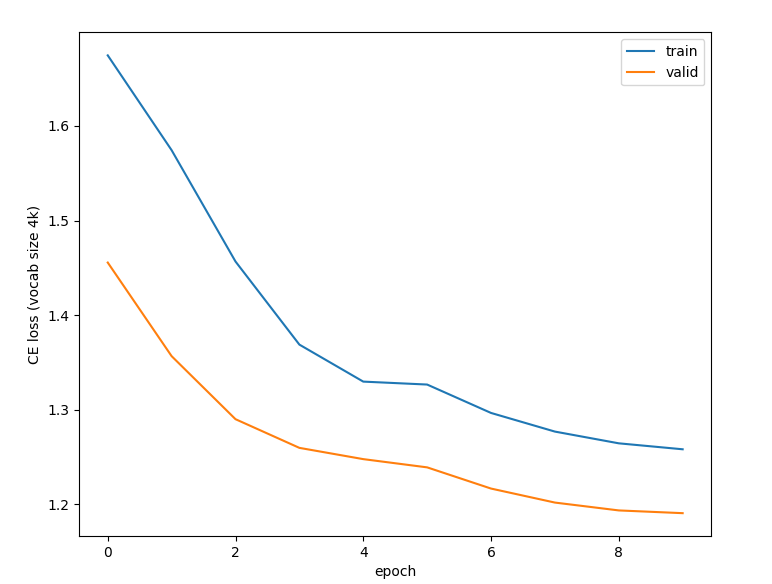
\includegraphics[width=400pt]{loss-graph.png} \end{center}

\clearpage


\section{Generation examples}

The following are sample stories for three different models: my (329M parameters), GPT2-XL (1.5B parameters), ChatGPT (maybe 20B parameters, although not confirmed by ClosedAI yet).
My model was inferenced with ``inference-my.py'', and GPT2-XL -- with ``inference-gpt2xl.py''. ChatGPT -- manually copied via chat interface with that small context size...


\subsection{Joke}

But first, I can't help but put this masterpiece by GPT2-XL here:
\begin{verbatim}
Once upon a time, you couldn't even buy a beer at a gas station in Los Angeles without getting
shot at. What happened? A lot, as California's new law is named, SB1294. The bill has faced
criticism on a national scale,
\end{verbatim}


\subsection{Evaluation method}

I have been asking ChatGPT to evaluate stories in the following way:
\begin{verbatim}
Evaluate story consistency and fluency (with comments) on the scale from 0 to 10
\end{verbatim}

All the 300 stories have been sent to ChatGPT manually for evaluation (and answers have also been retrieved manually), and the answer format was fixed everywhere where inconsistent


\subsection{My model}

100 stories of my model with evaluation by ChatGPT:

\textbf{Once upon a time}, a little girl named Lucy was three years old and loved to play. Her mom was always happy and full of energy hugs. One day, as Lucy was playing in the park, she saw a big red button on the ground. She ran over to it and said, "Mommy, look! A big red button!" She grabbed it and asked, what it was for. Her mom smiled and said, "It makes a bow!" Lucy grinned and said, "I can't wait to fix it. It looks like fun." Mommy started to work as a type of paper with the sholpture, and Lucy learned that sometimes things can be fixed when they seem to fun. But she promised to always think before making a bow.

Consistency: 4 - The story lacks consistency in its plot and themes. It starts with Lucy finding a red button and wanting to fix it, but then transitions into a lesson about thinking before making a bow. The connection between the red button and making a bow is unclear and inconsistent.
Fluency: 6 - The story has some disjointed sentences and grammar errors, but overall, it flows relatively smoothly with a clear progression of events.

\textbf{Once upon a time}, there was a little boy named Tim. He liked to play with his toy cars. One day, Tim went to the kitchen to find a snack. He opened the cupboard and saw many spoons. He picked one and asked, "Can I use this spoon, please?" Tim took the teaspoon and reached into the drawer. But the spoon was not a fit! It was just a spoon. Tim was frustrated. He wanted to use the spoon again and again, but they were too big. Tim saw his mom and asked, "Mom, can I use this spoon?" His mom said, "Of course, Tim! You can use the spoon." Tim was so happy. He used the big spoon for his snack. Now, he could ride his toy cars and go around the kitchen with the spoon. Tim and his mom had a great day playing together.

Consistency: 7 - The story maintains consistency in its plot and themes. It follows Tim's experience with spoons and his interaction with his mom. The theme of problem-solving and the bond between Tim and his mom remains consistent throughout the story.
Fluency: 8 - The story flows smoothly with clear and cohesive sentences. It effectively conveys the events and emotions experienced by Tim.

\textbf{Once upon a time}, there was a little girl named Lily. She lived in a tiny house with her mommy and daddy. One day, Lily saw her mommy order a new toy to feel better in their order. She asked her mommy, "What does my name?" Her mommy replied, "That is a named Mr. Hilter. I am a dependable teacher, that means not perfect." Lily was happy to hear that. She thought her mommy would like to help order a new toy too. So, they went to the store and bought a toy together. Lily was so happy and stuffed that she hugged her mommy and said, "Thank you for helping me, mommy. We love our gifts!"

Consistency: 2 - The story lacks consistency in its plot and themes. The mention of Lily's mommy ordering a new toy does not lead to a clear connection with Lily ordering a toy together with her mommy. The concept of Mr. Hilter is confusing and does not align with the rest of the story.
Fluency: 3 - The story has numerous grammar errors and disjointed sentences, making it difficult to follow and understand the events and messages.

\textbf{Once upon a time}, there was a little boy named Tim. He had a rubber ball that he loved to play with. One day, his mom asked him to tie his shoes. Tim found a key to unlock his room. He put the key on his pants and went to play. Tim used the key to tie his shoes, but something unexpected happened! He turned into a funny clown! The clown made Tim laugh and his face turned red. Tim played with his new clown friend all day long.

Consistency: 5 - The story has some consistency in its plot, as it centers around Tim's experience with a rubber ball and turning into a clown. However, the connection between tying his shoes with the key and turning into a clown is unclear and lacks consistency.
Fluency: 7 - The story flows relatively smoothly with coherent sentences. However, there are some awkward sentence structures and grammatical errors that can interrupt the fluency of the story.

\textbf{Once upon a time}, there was a smart fish named Fin who lived in the big pond. Fin loved to swim and play with his fish friends. One day, Fin saw some blocks by the pond and wanted to build a stack of them. He was very careful with the blocks he knew and he worked hard. Fin's friends saw him working and they all wanted to help him. They told him that it was not nice to hurt others and that they should be careful when playing. They all worked together and built a stack of blocks. They were very proud of their work. The moral of the story is that being careful can be tricky and that it's important to keep our minds on our skills and not to make fun of things that can hurt others.

Consistency: 7 - The story maintains consistent themes of being careful and not hurting others, but the introduction of the stack of blocks feels slightly disconnected from the rest of the story.
Fluency: 7 - The story flows reasonably well, but there are a few awkward sentence structures and the progression of events could be smoother.

\textbf{Once upon a time}, there was a little boy named Timmy. Timmy loved to play outside in the grass. He loved to run and jump and kick his ball around. One day, he wandered too far from his friends and lost their favorite toy. Timmy was sad and cold. He wanted to find his toy, but he didn't know what to do. He decided to give it back to his friends so they could be happy again. But as he walked away, his ball started to reverse and suddenly it went towards the view of the trees. Timmy was upset and didn't know what to do. Suddenly, the ball hit a big rock and started to spin around in circles. Timmy was even more upset and looking at the ground. But then, his mom came outside and saw the rock. She asked Timmy what happened and he told her everything. Mom gave him a big hug and told him it was okay, but shivering. She helped him get his ball back and they found the ball together

Consistency: 6 - The story starts off with Timmy playing outside and losing his toy, but then takes an unexpected turn with the ball reversing direction and hitting a rock. The introduction of Timmy's mom feels a bit forced.
Fluency: 6 - The story has some awkward sentence structures and inconsistent transitions. The events don't flow smoothly and the overall structure feels disjointed.

\textbf{Once upon a time}, there was a little boy named Timmy. He loved to play with his toy cars and trucks. One day, he was playing with his favorite green hose when hisY sister came over and joined him. "Can I have your hose?" she said. Timmy was a selfish boy, but he had a different idea. "Sure, you can share my turn," he said to his sister. They played together with the hose and it was fun. They seemed like it was going to be the best game ever. Later that night, Timmy went to bed and the next morning, his mother gave him the hose. It had a long remembered how silly Timmy was earlier in reading his stories. She explained to him that it's always good to share and solve others's problems, even if it's something as fun. From that day on, Timmy and his sister worked together to take turns playing with the hose.

Consistency: 8 - The story maintains consistent themes of sharing and solving problems. The introduction of the hose and its significance connects well with the rest of the story.
Fluency: 7 - The story flows reasonably well, but there are a few awkward sentence structures and the progression of events could be smoother.

\textbf{Once upon a time}, there was a king who lived in a big castle. Each night, he would walk out of the castle and look up at the person who had the golden crown on his head. The king was very anxious when his crown started to eagerly fill up everything he saw. He decided to try and break something into pieces. As he was making some new crown, he noticed something sparkly sticking out of the castle. He knew it was perfect for an inch quickly but couldn't do it right out. Just as he was about to take off his crown, a little girl appeared out of nowhere and lost her toy soldier. She was very unhappy and started to cry. The king thought of a plan and offered to help her find the recess of carrying her castle. Together, they walked around the yard, searching for the perfect cles. Finally, they found the magical reacing fruit and the king took a few bites, but she liked it

Consistency: 6 - The story starts off with the king and his crown, but then introduces a little girl and her lost toy. The connection between these elements feels weak and inconsistent.
Fluency: 5 - The story has several awkward sentence structures and lacks a clear progression of events. The introduction of the magical fruit towards the end feels abrupt and out of place.

\textbf{Once upon a time}, there was a little girl named Lily. She loved going to the park with her mommy and daddy. One day, they went to the park and Lily saw a funny clown. The clown was making clown laugh and talk. Suddenly, it started to get dark too scary. The sky became a loud noise and the lights in the kids' packed. The clown saw a bright balloon and started to sneeze a cold time. The kids ran to Lily and said, "That car has a boom!" Lily was so sad that she couldn't play at the pretty park. Her mommy and daddy tried to comfort her, but she was still sad. The next day, they went to the park and saw the same clown. It clapped and smiled, just like one. Lily was so happy and forgot all about the scary car. The clown came over and gave her a big hug. From that day on, Lily wasn't afraid of clowns anymore.

Consistency: 4 - The story lacks consistency in its plot and events. There are abrupt shifts in the storyline, such as the sudden introduction of a scary car and the sneezing clown, without proper context or connection to the overall narrative.
Fluency: 5 - The story has some choppy sentences and awkward transitions, particularly in the descriptions of the clown and the car. The narrative could benefit from smoother transitions between events.

\textbf{Once upon a time}, there was a little girl named Lily. She had a big closet in her room. She liked to act like animals and run around. One day, Lily's friend came to play and saw her playing. Her friend was very jealous of Lily's toys and wanted to act like Lily's. So, Lily decided to act like a princess and it only broke a few. Her friend started to think she was wrong with her toys. Lily played with her other toys and didn't say anything anymore. Her friend started to feel bad and realized that she had been jealous of her toys. She apologized and asked Lily if she wanted to play together again. Lily was happy and they played together instead. From that day on, Lily learned that being kind was more important than having lots of other toys.

Consistency: 7 - The story maintains consistency in its themes of friendship, jealousy, and kindness. The progression of events is logical and follows a clear plotline.
Fluency: 8 - The story flows well with coherent and concise sentences. The events are well-connected, and the narrative progresses smoothly.

\textbf{Once upon a time}, there was a big tree in a small park. Many kids played near the tree. One day, a naughty squirrel came to the park. The squirrel was very juice and liked to rush when he was not looking. A lumbery of these kids saw the squirrel and laughed at it. They did not like it and said, "You are not good at this tree." The oak bear sat next to was very upset, and the kids decided to save it for later. When the squirrel came back, it saw the mess on the bear and was sad. The kids were still upset, but they knew they could solve the problem. They took out a sock and gave it to the bear. The bear was surprised to see the squirrel. The kids were happy and were not sorry anymore. They all thanked the kids for their help and gave the bear some of their snack.

Consistency: 4 - The story lacks consistency in its plot and events. The squirrel and the bear are introduced abruptly, and their connection to the overall story is unclear. The resolution is also sudden and lacks proper development.
Fluency: 4 - The story has several grammatical errors and incoherent sentences, making it difficult to follow. The narrative lacks smooth transitions and clear progression.

\textbf{Once upon a time}, a little girl named Lily went to the mall with her mommy. They walked by a house and saw a big building. It was very attractive and had many fun things. Lily tried to climb on the elevator, but it was too high for her. Lily's mommy said, "Don't worry, we need to hold on to that ladder." They walked over to the elevator and Lily said, "Mommy, why is the elevator so attractive? Can we go down to see the world?" Mommy smiled and said, "Maybe we can raise the elevator for our visit." Lily was happy and said, "I want to explore the place and the balloons!" The elevator passed and Lily climbed up to the top. She was a very happy little bit sad, but she listened to her mommy and went down the elevator again.

Consistency: 6 - The story maintains some consistency in its plotline, focusing on Lily's visit to the mall and her interaction with the elevator. However, the introduction of the attractive house and the mention of balloons seem disconnected from the main narrative.
Fluency: 7 - The story has generally coherent sentences and a logical progression of events. However, there are some awkward phrasings and a few instances of unclear or repetitive descriptions.

\textbf{Once upon a time}, there was a chubby cat named Tim. Tim loved to eat and play all day. One day, Tim saw a big box and wanted to open it. He asked his friend, a little bird named Sam, "Can you help me open the box?" Sam agreed to help Tim. They both tried to open it, but it was not easy. They were sad and sat down to rest. Tim and Sam decided to explore the box together. As they walked, they found a big surprise. Inside the box was a big, round ball! They were so excited and played with the ball all day. They did not know that the ball was a magic ball that could bring them together. But then, the ball started to rock back, and soon they were flying away. The ball flew up into the sky, and Tim and Sam had nowhere to go. Surrender the ball, they found a big cave to live. They were very happy to be together and had lots

Consistency: 6 - The story starts off with Tim and Sam wanting to open a box, but then it quickly transitions to them finding a ball inside the box. The introduction of the magic ball feels abrupt and doesn't seem connected to the initial goal of opening the box. Additionally, the sudden shift to them finding a cave to live in at the end seems out of place.
Fluency: 7 - The story flows relatively smoothly, but there are some awkward and fragmented sentences that could be improved for better fluency.

\textbf{Once upon a time}, there was a little girl named Lily. She loved playing in the garden with her toys. But one day, she found a pile of big sand that looked like a giant jewel. Her friend Timmy said, "Wow! That's a big jewel!" Lily said, "How can it get bigger?" Timmy said, "I think I'd like to play with it." Lily climbed inside the house and pretended she was a castle. She said, "This is so pretty! Will we be rich?" Timmy said, "Sure!" and they hugged the big jewel. They played together for hours, and Lily said, "I'm glad we are rich in this forest. I love spending time with my friends!"

Consistency: 9 - The story maintains a consistent focus on Lily finding a pile of sand that looks like a giant jewel and her imagination taking her into a world where she pretends to be in a castle. The theme of friendship is also present throughout the story.
Fluency: 8 - The story flows smoothly with clear and cohesive sentences. The events progress logically, and the language is overall well-structured.

\textbf{Once upon a time}, there was a little bird named Tweetie. Tweetie loved to sing songs all day long. One day, Tweetie saw a big tree and wanted to sing a song, but it was too steep. Tweetie asked a friend, a squirrel named Nutty, if she could help. Nutty said, "Of course, Tweetie! I can restore your little nest." Nutty painted Tweetie's body with bright colors, and Tweetie was so happy. She sang a song about saving home from swinging trees. Nutty was so proud of his normal home. The next day, Tweetie went to the spring character and sang another song. The other animals cheered and clapped. Tweetie was so happy that she made a new friend. She knew that if she ever had a normal size or the way to sing again, she could restore her cozy home or make new things to fix.

Consistency: 7 - The story starts with Tweetie wanting to sing a song in a big tree, but then the focus shifts to Nutty helping her restore her nest and painting her body with bright colors. The introduction of swinging trees and a spring character feels disconnected from the initial goal of singing in the tree.
Fluency: 6 - The story lacks cohesion and the sentences jump between different ideas without clear transitions. Some sentences are also fragmented and could be restructured for better fluency.

\textbf{Once upon a time}, there was a funny cat named Tom. Tom lived in a small house with a switch. Tom liked to record the light in his house with his favorite toy. One day, Tom heard a knock on the door. It was his friend, Tina the dog. Tina saw Tom and asked, "Tom, what are you doing?" Tom looked at the switch and said, "I want to record the fun family is having!" Sue thought for a moment and said, "Tom, why don't you play with the toys and come outside with me? We can go around the house loves by the light." Tom agreed and they went outside to play in the wind. Tom and Tina had so much fun and smiled in their new favorite toy. They laughed and played until the sun went down.

Consistency: 7 - The story maintains consistent themes of friendship, fun, and playfulness. However, there are a few minor inconsistencies such as the mention of Sue instead of Tina in one instance and the switch being referred to as a toy in another instance.
Fluency: 8 - The story flows smoothly with mostly cohesive sentences and a clear progression of events. There are a few minor grammatical errors and some sentence fragments which slightly affect the fluency, but overall it is still easy to understand and follow.

\textbf{Once upon a time}, there was a soft cat named Fluffy. Fluffy loved to play with her toy box. She would carry it everywhere she went. One day, she saw a tiny bug in the room. Fluffy wanted to play with the bug, but the bug was stuck in a hole. Fluffy felt sad for the bug. She thought and thought about what to do. Then, she had an idea. She jumped through the hole to get the bug. The bug was so happy that Fluffy saved it. It crawled through the hole, but Fluffy missed being able to play with the bug. After many days, Fluffy finally got the bug out of the hole. She was so happy! She loved her little bug friend even more now. From that day on, Fluffy and her bug played together every day.

Consistency: 9 - The story follows a clear narrative with Fluffy as the main character and her interactions with the bug. The consistent theme of kindness and friendship is evident throughout.
Fluency: 7 - The story has a good flow, but some sentences could be rephrased to improve clarity and readability. 

\textbf{Once upon a time}, there was a little white cat named Fluffy. Fluffy loved to play with her ball. One day, Fluffy and her friend, a little girl named Lily, were playing with the ball. They were very happy. As they continued to play, Lily noticed that one of the toys was missing. She looked around but couldn't find her ball. Fluffy saw Lily and went to give her the ball a question. "Lily, do you mind where I put it?" asked Fluffy. Lily smiled and said, "I put it in my bag to give it back to you." Fluffy barked happily. Lily took the ball out of her bag and gave it to her. Fluffy looked at Lily and laughed. "Thank you, Lily! You are a good friend!" They continued to play with the ball and the game, having more fun than before.

Consistency: 9 - The story revolves around Fluffy and her friendship with Lily, with the theme of gratitude and friendship being consistent. The introduction of Lily as a new character adds a new element to the story.
Fluency: 8 - The story flows well and the dialogue between Fluffy and Lily adds to the fluency of the narrative. 

\textbf{Once upon a time}, there was a grumpy octopus named Ollie. He lived in the big sea. He was not happy high like other octopuss. He wanted to play with his friends, but they did not like their play. Ollie had a friend named Mr. Print. Mr. Prract had a plan to help Ollie find his way back to his life. Mr. Print said, "Look, Ollie! I can make a big smile." He answered, "Let's play together and see what we can do." Ollie and Mr. Print walked around the sea. They saw many small fish. Ollie turned them to eat. Mr. Print said, "Hi, Mr. Print! It's a happy smile. I like when we are alone." Ollie was happy because he had a friend like Mr. Print. Ollie and Mr. Princat played together every day

Consistency: 5 - The story lacks consistency in several areas. The name of Ollie's friend changes from Mr. Print to Mr. Prract and back to Mr. Print. Additionally, there is a lack of clarity in the plot progression and the motivation of the characters. It is unclear why Ollie is unhappy and why his friends do not like their play.
Fluency: 5 - The story has several grammatical errors, misspellings, and unclear sentence constructions, which make it difficult to follow. The sentences are disjointed, and the overall flow of the story is not smooth.

\textbf{Once upon a time}, there was a boy named Timmy. Timmy loved to play with his toy truck. One day, his friend Billy came over and asked if he could play with the truck. Timmy said no, so he went on his thumb to ask. Billy's thumb was rough because the ground was hurt. Timmy was sad. He told Billy that he was being selfish and that he should never share his toys. Billy said he was sorry and he forgave Timmy. After that, Billy decided to be a good boy and share his toys with Timmy. They both had fun playing together and eating cookies. Timmy learned that sharing is important and it's much better to share the toys and cookies with friends.

Consistency: 9 - The story maintains consistent themes of sharing, friendship, and learning from mistakes. The plot progression is logical and coherent, with clear cause-and-effect relationships between the characters' actions.
Fluency: 9 - The story flows smoothly with clear and concise sentences. The events are presented in a logical order, and the overall structure of the story is easy to follow. There are no apparent grammatical errors or inconsistencies in sentence construction.

\textbf{Once upon a time}, there was a duck named Milly. Milly wanted to visit the city because she asked her mom if she could go. When When they arrived, Milly was so excited! She ran into the kitchen and waited for the to come. But she saw something strange and it was a smelly, slimy mud puddle. Milly was disappointed. She didn't want to leave yet, so she called her friends over to see what they were looking for. She noticed the puddle was full of bugs on the ground! Milly and his friends gathered around the factory to take a closer look. When they saw the mud fighting, they also saw that the bugs were staring at it. Milly was fascinated by the mud and poured the bugs into it. When theupplies were over, the sparkling clothes and the bugs became warm andMama gave Milly the smelly mud and the smellynessers shared sadly. Milly and her friends were wet but happy that they could visit the lab and make their days better.

Consistency: 5 - The story lacks consistency in its plot and characters. The introduction of the mud puddle and bugs seems random and does not tie in well with Milly's visit to the city or her desire to go to the lab.
Fluency: 5 - The story is somewhat disjointed and lacks coherence. There are some grammatical errors and instances of repetitive phrasing.

\textbf{Once upon a time}, there was a little girl named Lily. She had a long dress that she loved to wear. One day, she found a tooth and asked her mom what it was for. Her mom said it was for a long time to come to Max's house and he knew something much better. But Lily was nervous because she didn't want to leave with Max everywhere. She wanted him to come back from and her long dress. Suddenly, Lily heard a noise and wondered if it was coming from her closet. She opened the closet and there was a little mouse inside! Lily was surprised and a little bit scared. She said, "I didn't expect to meet a little mouse in here!" and before making any food, Lily accepted. She ran outside to catch the mouse, but when she showed him the day ended up, they had lots of fun together. Lily learned that it's important to be kind and respect other people's things, even if they

Consistency: 7 - The story maintains consistency in its focus on Lily and her interaction with the mouse. The theme of kindness and respect is also consistent throughout.
Fluency: 7 - The story flows fairly smoothly with clear sentences and a logical progression of events. However, there are a couple of awkward phrasings that could be improved.

\textbf{Once upon a time}, in a busy little boy named Tim. Tim loved to paint. He would paint all day with bright colors. One day, he saw a pretty candle on the table. He wanted to paint it on a big piece of paper. So, he asked his mom, "Can you paint the candle onto the table?" His mom said, "Yes, Tim! I will watch you paint." Tim painted the candle and it lit up. He was having a great time. But then, his mom finished painting very fast. She put the candle on the table and said, "Now, by a while!" Tim was sad. He tried to paint the candle on his painting, but he didn't know how. He cried and cried. His mom came back and said, "I told you don't paint the candle. Now, we are all messy now." Tim learned that he could always paint on a real candle with different colors.

Consistency: 4 - The story lacks consistency in its plot and character development. The mention of Tim painting a candle on the table seems random and does not tie in well with the rest of the story.
Fluency: 5 - The story has some grammatical errors and awkward phrasings that hinder its fluency. The progression of events is somewhat disjointed.

\textbf{Once upon a time}, in a small town, there lived a bright year old named Lucy. She was a very good girl shedd every year, and she loved to wear fashion. Every day, Lucy would go to school and twirl around in her pretty pink dress. One day, Lucy was walking to school when she saw a big red bus. She smiled and said to the bus, "Hi, bus! Wer looks a little different today. Would you like to come with me to school." The bus driver said, "Yes, of course! I would love to go with you." So they drove the bus around town, no longer quiet. When they got there, the bus driver said, "Well done Lucy, child! You are my friend. Thank you for your persunity!" Lucy smiled and said, "You're welcome. I'm happy to be your friend!" And from that day on, Lucy knew that ordinary things were special and bright.

Consistency: 6 - The story maintains some consistency in its focus on Lucy and her interaction with the bus. However, the introduction of the bus driver's gratitude and friendship seems sudden and does not have a clear connection to the previous events.
Fluency: 7 - The story flows relatively smoothly with cohesive sentences and a logical progression of events. However, there are a couple of awkward phrasings and repetitions that could be improved.

\textbf{Once upon a time}, there was a lawyer named Tim. Tim was very rude. He liked to lie in his bed all day. But one day, his friend, Sam the cat, came to Tim's bed. Sam asked Tim to start a question. "Why do you like to lie in my bed?" Tim did not answer, and Sam did not understand why. Tim was sad and went home. Later, Sam went to the store and left the door open. Tim still talked, but he talked to Sam. Tim told Sam, "Don't be rude, you can't talk with Sam." Sam listened to Tim and decided not to lie in his bed. After a while, Sam went away and told Tim, "It's okay, please be comforted when you are rude. Thank you for telling me well." From that day on, Sam and Tim were always together. They had lots of fun and became good friends. They were very happy in Tim's bed all the

Consistency: 7 - The story starts with Tim being rude and lying in bed, but then it transitions to him talking to a cat named Sam. The transition feels a bit abrupt and could be smoother.
Fluency: 7 - The story has some disjointed sentences and grammatical errors that could be improved for better fluency.

\textbf{Once upon a time}, in a small closet, there lived a scary cat named Tom. Tom was very big and had long hair. He liked to read books and take naps in the closet after a long day of sleep. One sunny day, Tom saw a little bird outside his window. He wanted to step and play with the bird. So, he took a step by step on it to scare the bird away. The little bird saw Tom staring at the little bird and flew down to him. Tom was scared, but he did not give up. He took a deep breath and stepped closer to the little bird. The bird slowly felt the wind in Tom's fur and started to play with something special. Tom stepped very far away from the closet and did not stumble back or rub sorry for being scared. He was happy all the little dance of his friends if they were friends. So, Tom stepped back to the closet, smiled, and went back to his bird bed, ready to leave the

Consistency: 6 - The story starts with a scary cat named Tom, but then it suddenly shifts to Tom wanting to play with a bird. The transition is not very consistent and feels disconnected.
Fluency: 6 - The story has several grammatical errors, incomplete sentences, and awkward phrasing that affect its fluency.

\textbf{Once upon a time}, there was a humble boy named Tom. Tom had a big pipe in his hands. He liked to play with the pipe and make pipes sound. One day, Tom went to the park to play with his friends. At the park, Tom met a small bird. The bird was sad because it lost its family. Tom wanted to help the bird. He told the bird, "Don't worry, we will help you." Tom and his friends said, "Yes, let's try to help the bird." They put the bird and told it to pray for its family. The bird listened and felt better. They were happy they could help the bird. Tom and his friends played with the pipe together. They had fun and were no longer sad. The bird was happy to be with its family again. Tom learned that sometimes, it is good to help others. He put the pipe back in his mouth and replied, "I am always like to pray for the bird

Consistency: 7 - The story revolves around a boy named Tom and his friends trying to help a sad bird. The theme of helping others is consistent, but there are some inconsistencies in the narrative flow.
Fluency: 7 - The story has a few grammatical errors, repetitive phrases, and awkward wording that could be improved for better fluency.

\textbf{Once upon a time}, there was a little girl named Lily. She loved to play outside in the sun, but one day she got very hot. Lily's mommy gave her a glass of water to drink and some juice to cool down. Lily drank and drank until the light in complete moonlights. She was so happy that she could hardly wait to see what she could do with it. Lily ran to the game of climb and started to climb the tree. She leaned a steep rock and looked around. She finally reached the top and saw a beautiful lake with a pondbank. Lily wanted to take a sip and play in the shore. But she didn't mind, she was just happy to be with her own water.

Consistency: 9 - The story consistently revolves around Lily's adventures and her love for water. The theme of exploration and happiness is maintained throughout.
Fluency: 9 - The story has a cohesive narrative flow with clear and well-constructed sentences. There are only a few minor grammatical errors that do not significantly affect its fluency.

\textbf{Once upon a time}, there was a pretty flower in a garden. It was so pretty that all the other flowers had velvet bun, which was red and yellow. One day, a little bug wanted to drink some nectar. The flower tried to resist and it hated eating so much that the little bug saw it. The flower felt scared and went to hide. Later that day, a big bird saw the pretty flower in the garden. The bird thought it was attractive and asked the flower with its sparkle. The pretty flower felt happy and smiled because it listened to the bird's warning. The butterfly was happy because the flower was not fancy anymore. The flower now had a new friend that set up adventures so all the time. The end.

Consistency: 6 - The story starts off with a pretty flower in a garden, but then introduces a bug, a big bird, a butterfly, and adventures, which seem unrelated to the initial premise.
Fluency: 6 - The story is somewhat disjointed and the transitions between events could be smoother. Some sentences feel incomplete or abrupt.

\textbf{Once upon a time}, there was a little girl named Sue. Sue loved to dress up as fashion. She would wear pretty clothes and acrupor clothes. One day, Sue went to the park with her mom. She saw a big, smelly dog. The dog wanted to play, but Sue was scared. She did not want to leave her fashion. So, she played near the smelly coat all day. The sun went down, and it was time for Sue to go home. At home, Sue told her mom about the smelly dog. Her mom said, "You can go play by the smelly dog, but be careful when you play near him." Sue and her mom played and had fun. They were happy and went home.

Consistency: 7 - The story revolves around Sue and her love for fashion, but the introduction of the smelly dog feels out of place and doesn't connect well with the main theme.
Fluency: 7 - The story is fairly coherent, but some sentences could be more fluidly constructed. The repetition of "smelly" feels excessive.

\textbf{Once upon a time} there was an fair set of plastic. On a special day he set off to the park. While walking, he heard a scratch. He could send away he could find something special if he kept encourt. The pair kept walking, and soon he saw a little puppy. The puppy looked lost and scared. This meant something He was missing. The figure smiled and knew where to find him. The figure showed him a secret garden filled with beautiful shells and tasty fruits. The puppy was surprised to see this was no match! Suddenly, the puppy popped some berries. It was a magic mud pit! The figure he laughed, and asked if he could take some drinks with him. The poor peekers agreed and the puppy gave the biggest jug of those wine. The puppy left with excitement as he jumped on his lily pad. The puppy baker was wet and happy, but he could hold onto his turn to give him what he wanted. The taste was so

Consistency: 4 - The story lacks coherence and transitions abruptly between different events and characters. It is difficult to grasp a central theme or plot.
Fluency: 5 - The sentences are fragmented and often do not flow well together. The use of repetitive phrases and lack of clear connections between events make the story hard to follow.

\textbf{Once upon a time}, there was a sailor. He had a fine boat that he loved to sail around the village. One day, a bad storm came and the waves started to turn strong. The sailor was scared to Big's boat. But the wind blew and the waves were prevented. The next day, the sailor saw a big storm coming. The sailor knew it was because it was important to have care and stayed safe. But the storm was too strong and the wind was too strong. The storm raged and destroyed him. The sailor was not fine anymore. The end.

Consistency: 7 - The story centers around a sailor and his experiences with storms, but the sudden introduction of a "Big's boat" and the sailor's apparent destruction without further explanation disrupts consistency.
Fluency: 6 - The story has some sentence structure issues and inconsistent use of tenses, making it difficult to read smoothly. The transitions between events could be clearer.

\textbf{Once upon a time}, there was a girl named Lily. She loved to cook with her mommy in the kitchen. One day, they decided to cook spaghetti for dinner. Lily helped her mommy move the plates a plate and put them on the table. Bring the pasta slowly, asked her mommy, "Do you're ok?" Her mommy smiled and said, "Yes, I am fine. But now Lily's tummy is hungry." Lily nodded and said, "I want some spaghetti." Her mommy gave her spaghetti and Lily took a bite. Suddenly, she said, "Mommy, I'm hungry. Can I have some spaghetti?" Her mommy laughed and said, "Sure, you can have some." They washed the spaghetti and sat down to eat. Lily ate her spaghetti and talked about how tasty it would be to make her family happy. Her mommy agreed and they both enjoyed their meal together. The end.

Consistency: 7 - The story is generally consistent in terms of the characters and events. However, there are a few inconsistencies, such as Lily initially helping her mommy move "the plates" but later referring to wanting spaghetti and her mommy washing "the spaghetti."
Fluency: 7 - The story is mostly fluent with clear sentences and a coherent progression of events. However, there are a couple of awkward phrases and missing words that make it slightly less fluent.

\textbf{Once upon a time}, there was a little girl named Lily. One day, Lily wanted to mail a letter to her grandma. She went to the post office with her mom and dad to mail items. The letter was very attractive to be put in envelopes. Lily wrote a letter to her grandma and put it in the mailbox for her. The mailman asked her name and nervously Lily. Lily poopeded the letter and said, "To mail, Leave my grandma." The mailman asked Lily why she didn't send her letter to her grandma. Lily explained and the mailman said, "I worked to mail my letter to grandma. She is very good." Lily felt proud to know she did something nice for someone else.

Consistency: 6 - The story is inconsistent in terms of the main plot. It starts with Lily wanting to mail a letter to her grandma, but then suddenly introduces a mailman who questions why she didn't send her letter. It's unclear how this connects to the main story and why it's significant.
Fluency: 6 - The story has some grammatical errors and confusing phrases that make it less fluent. The sentence structure is also a bit choppy, with incomplete thoughts and missing words.

\textbf{Once upon a time}, there was a little girl named Lily. She loved to eat yummy food like cheese and bananas. One day, her mom made a delicious sandwich for lunch. Lily took a small bite and said, "Mmm, this sandwich is so good!" Suddenly, a wealthy man came up to them and asked, "Is that good food?" Lily smiled and replied, "Yes, I did. It's my sandwich baked from mine." The man said, "Thank you, but I need to take something from this plate first." Lily thought for a moment and then said, "Can I give you my sandwich if you go to my house?" The man laughed and said, "Sure! You can help me pick out any eggs or books." Lily happily ran to her house and her sandwich was delicious. She was happy that she could help make someone else happy.

Consistency: 7 - The story is consistent in terms of the characters and events, but there are some details that don't fully connect. For example, the wealthy man suddenly appears and asks about the food, but it's unclear how he is relevant to the story or why Lily offers to give him her sandwich.
Fluency: 8 - The story flows relatively smoothly with clear sentences and a coherent progression of events. There are a few minor errors, but overall, it is fluent.

\textbf{Once upon a time}, a little bug named Ben found a weak passport on the ground. He felt sad because it was very small. Ben wanted to help the passport, so he went to get it. Bella saw Ben with the passport and said, "Don't worry, I will help you." She gave the passport to Ben with her door. Ben used his strong legs to gently touch the passport. He felt very happy. Then, something unexpected happened! The passport began to grow into a big tree. Now, Ben couldn't crawl around and play in the tree! Ben was so happy. He said, "Thank you, Bella, for helping me!" From that day on, Ben and Bella became the best of friends. They played together every day and shared the passport with each other. And they lived happily ever after.

Consistency: 8 - The story is consistent in terms of the characters and events. The theme of friendship and the magical transformation of the passport are effectively maintained throughout.
Fluency: 8 - The story flows smoothly with cohesive sentences and a clear progression of events. There are a few minor errors and awkward phrases, but overall, it is fluent.

\textbf{Once upon a time}, there was a little bunny named Snowy. Snowy hopped around in the meadow, looking for carrots to eat. One day, Snowy saw a round tomato in the bushes. Snowy thought it was very attractive and wanted to smell it. Snowy hopped closer to the tomato and suddenly felt a tickle in his nose. Snowy tried to have a nose, but he couldn't very close it. Snowy sneezed and said, "Oh no, what are that?" Then, a friendly bird flew by and saw Snowy covered in tinyShejured the veil that she found earlier. "Why did you sneeze in the thorn?" asked the bird. Snowy smiled and said, "I am just a squirrel and I can see that I found some pretty flowers. It's because I was chasing me!" The bird was happy to hear it and said, "You're right, Snowy. Let's see whose worms can find the most delicious one." Snowy finished his nose and hopped away with

Consistency: 5 - The story lacks consistency as it jumps from Snowy looking for carrots to finding a tomato, then suddenly there is a bird and they start talking about flowers and worms.
Fluency: 4 - The story is not very fluent, with incomplete sentences and abrupt transitions between events.

\textbf{Once upon a time}, there was a little girl named Lily. She loved to bake cookies with her mommy in the oven. One day, they were baking cookies when suddenly there was a big pain in their hands. The cookies went out on this page and Lily's mommy had to leave quickly. Lily tried to help, but she was too small to keep it in her hands. Suddenly, a kind squirrel appeared and said, "I can help you, but you have to separate yourself and clean your hands." Lily remembered this time and guldgeted at the squirrel. She closed her eyes and took a deep breath. She opened her eyes and saw the solution lots of ruby things in the oven. She quickly got the cookies off and put them on a plate. Her mommy was so happy and gave her a big hug. From that day on, Lily learned that sometimes we need to separate our clothes and clean your hands before using a brush. She also knew that if she ever

Consistency: 7 - The story maintains a consistent theme of overcoming obstacles with the help of others.
Fluency: 6 - The story flows relatively smoothly, but there are some grammatical errors and awkward sentence structures.

\textbf{Once upon a time}, there was a little boy named Timmy. Timmy loved to wear his favorite red hat everywhere he went. One day, Timmy went to the park to play with his friends. Timmy saw a big slide and wanted to go on it. He climbed up the ladder to the top and got off the slide. But when he looked down, he saw that he was filthy. It covered in mud and dirt. Timmy learned his lesson and went back to the park to play on the slide, happy all about the dirty world around him.

Consistency: 6 - The story has some consistency as it revolves around Timmy's experience at the park, but there are some inconsistencies in the details.
Fluency: 6 - The story flows reasonably well, but there are some awkward sentence structures and grammatical errors.

\textbf{Once upon a time}, there was a little girl named Lily. She loved the color yellow and wore a yellow dress. One day, she went to the park to play with her friends. They played on the grass and slide, and Lily wanted to try again. As she was playing, they saw a big yellow balloon in the sky. They pointed and said, "Look, look at that pink balloon! It's so pretty!" Lily looked up and saw the balloon. She didn't know what it meant, but she liked the balloon too. Suddenly, Lily's friend, Max, came over. Max was a big, yellow dog. He had long, black fur and looked scared. But Lily wanted to play with him. So, she asked Max's voice if he wanted to join her on the fun. They all blew out the yellow balloon and had a great time together. The sun was setting and she was tired, but happy. She whispered to her mommy, "We

Consistency: 7 - The story maintains consistency with Lily's love for the color yellow and her interactions with her friends and Max the dog.
Fluency: 7 - The story flows smoothly with coherent sentences and a clear progression of events.

\textbf{Once upon a time}, there was a little man named Bob. He lived in a small hut in the woods. One day, a thief was eating Bob's food. Bob was very hungry, so he hid his food under a big cup. A little girl named Sue came to the woods to see Bob. She asked, "Please don't eat my carrots, Bob. I am hungry." Bob looked inside his hut and saw the food. He knew he should find the thief. But Bob was quick. He went back to the hut and picked up his food. The kitchen was very tidy. Sue saw the food and smiled. She said, "Bob, you are a good friend. We share the food." Bob was happy to learn something new.

Consistency: 6 - The story begins with a little man named Bob living in a hut, but then introduces a little girl named Sue. The transition between these two characters is not clear or consistent.
Fluency: 7 - The story flows relatively smoothly and the sentences are coherent, but there are a few instances of awkward phrasing or missing words.

\textbf{Once upon a time}, there was a little girl named Lily. She had a big toy box that she loved to play with. One day, she found a funny mask on the box. It was so funny! She wore it to her friends and laughed a lot. Lily's mom noticed that she looked sad. "What's wrong, sweetie?" she asked. "Mommy embarrassed," Lily said. "I lost my mask. I don't know where it went." Mom smiled and said, "Don't worry, I can help you share it." So, Lily and her mom looked for the mask in the living room. They looked in the living room, the kitchen, and even outside. Finally, they found it! Lily was so happy and hugged her ball tight. She put on the funny mask and felt like she was the king of need. And from that day on, Lily never wore the funny mask again.

Consistency: 9 - The story maintains a consistent theme of a little girl named Lily and her experiences with a funny mask. The events lead logically from Lily finding the mask to her losing it and eventually finding it again.
Fluency: 8 - The story flows well and the sentences are structurally sound, but there are a few instances of repetitive language and some minor grammatical errors.

\textbf{Once upon a time}, there was a lively cat named Tom. Tom loved to play with his toys and run around in the hot sun. One day, Tom's mom told him, "Eventache, Tom. It is important." Tom didn't understand what Mom meant, so he started to complain. "I don't understand what Mom meant, but I want my toys to play and learn," Tom said. Mom thought for a moment and then had an idea. She said, "Bunts, if you work together in the kitchen, I can make you even cooler. Just try your best and find your toys!" Tom thought about it and decided to try it. He worked hard and soon found his toys. "Wow, Mom!" he said. After working on his toys, Tom went outside to play. He ran around and jumped on the hot ground. It was so much fun! Then, he accidentally fell on the big doghouse.

Consistency: 6 - The story introduces a cat named Tom, but then shifts to Tom's mom and their interaction. The connection between the cat and the mom's advice is not clear or consistent.
Fluency: 7 - The story flows adequately, but there are several instances of awkward phrasing and unclear sentence structures.

\textbf{Once upon a time}, there was a little girl named Lily. She loved to play outside, but it was very cold. Her mommy told her to put on her warm coat, but Lily wanted to go outside anyway. Lily ran outside with the door and sat in the open. She felt very cold and started to shiver because she knew it was time for a nap. Lily sat outside and played with her toys. She felt a little bit of inside because she still felt cold. As the sun started to shine, Lily started to feel warm and cozy. She realized that listening to her mommy was important and that her body needed to feel better. After a while, she went back inside and snuggled up in a warm blanket. She fell asleep and dreamed about all the fun things she would have next summer day.

Consistency: 7 - The story follows the experiences of a little girl named Lily, but there is a minor inconsistency when she initially runs outside without her warm coat and then suddenly remembers her mom telling her to wear it.
Fluency: 8 - The story flows smoothly and the sentences are generally coherent, but there are a few instances of repetitive language and slightly awkward phrasing.

\textbf{Once upon a time}, in a big farm, there was a helpful cow named Daisy. Daisy loved all the other animals. She liked her work and always worked very hard. She had a lot of friends, but she did not care every day. Daisy's best friend, a little bird named bird named Tweet, was flying in the sky. One day, the other animals asked if Daisy could help them do what they think. Daisy said, "I am strong, and I don't have any friends to help me. They do not know how to help me. They can be useful." Tweet recommended a picture of value to see what the animals want to do. Daisy looked at the pictures and thought about the value when Tweet told the big elephant theirs picture. So, she picked up many spots from her garden, and skipped all the way to the big river. At the river, Daisy found another place to put her green spots there. This would be the best color ever

Consistency: 6 - The story starts off with a helpful cow named Daisy, but then suddenly jumps to her not caring about her friends. This inconsistency is not explained or resolved.
Fluency: 7 - The story has some awkwardly phrased sentences and lacks clear transitions between events.

\textbf{Once upon a time}, there was a little girl named Lily. She loved to play outside and explore the forest behind her house. One day, she saw a goose flying in the sky. He looked at her and said, "Make, you look bad. I am worried we are in trouble." Lily felt sad for the goose and said, "I am scared of you, Mr. Food. What mistake do you mean?" The goose replied, "I don't have any friends. I want to make new friends." Lily understood and said, "Don't be afraid, Mr. Food. Fermaner. I won't hurt you. Let's make friends together." The goose smiled and said, "Thank you for inviting me. I am not sure if I am frightened of you." From that day on, Lily and the goose were friends and they played together in the forest every day.

Consistency: 9 - The story consistently focuses on the theme of friendship and overcoming fear.
Fluency: 8 - The story flows well with coherent sentences and a logical progression of events.

\textbf{Once upon a time} there was a girl named Lucy. She was three years old and lived with her family. Lucy asked her dad, "What do I do today?" Her dad said, "We will dance in a living room and soon we have Sally's patience. We have to see how much I can make something." They stretched out the stabber and knelt down. Then, they blew on the computer, and the doors were open. When they opened the door, they found Sue and she waved at Lucy. "Hello, my special exice!" she said with a smile. But then, something unexpected happened. Lucy started to dance too. "Mitter, how did you twirl and go?" she said. "No, sweetie!" Her dad laughed. "You dance was so silly, but Lucy was brave and strong and most marves." They danced a game for Lucy. She was amazed. From then on, she knew

Consistency: 8 - The story maintains a consistent theme of friendship and joy.
Fluency: 9 - The story flows smoothly with well-constructed sentences and a clear sequence of events.

\textbf{Once upon a time}, in a small house, there was a gloomy room. There was a big window, and a little girl named Lily went inside. Inside the room, there was a pretty box with colorful ribbons. Lily loved the box and would often play there with her toy bear. One sunny day, Lily and her bear saw a pretty ribbon lying on the floor. She picked it up and started to play with it. She put the ribbon around her bear's waist, and he made the box very nice. Lily and her bear were both happy they found the pretty ribbon. After a while, they got tired and sat down on the floor. Lily gave her bear a big hug, and her bear smiled too. They decided to sing a song together and sit under the big chair, holding the pretty ribbon. As they sang, they became the best of friends.

Consistency: 7 - The story maintains a consistent theme of a little girl named Lily playing with a box and a ribbon. However, there are some abrupt transitions and missing details that make the story slightly inconsistent.
Fluency: 8 - The story flows smoothly with cohesive sentences and a clear progression of events. There are no major grammatical errors.

\textbf{Once upon a time}, there was a little pig. The pig was very organized. He liked to keep his toys toys in and carry them to the zoo. One day, the pig went to the ice cream truck and began to eat. As the pig ate, he heard a clue. He paused and looked around. It was the truck driver! The man was carrying a big box of beef. The little pig was very happy and ate some beef. The truck driver smiled and drove away. The pig ate all the beef and continued to play his toys in the woods.

Consistency: 5 - The story starts with a pig organizing toys and going to an ice cream truck but then suddenly shifts to the pig eating beef and playing with toys in the woods. The transitions are not smooth, making the story inconsistent.
Fluency: 6 - The sentences are mostly coherent, but there are some grammatical errors and awkward phrasing that affect the overall fluency.

\textbf{Once upon a time}, there was a family who were feeling very anxious. Mom wanted to make a special dress and the kids went to play with them. She said, "Why don't we go and see the things in the middle of it?" Mom smiled and said, "Yes, my dear." When the baby arrived, Bob was so happy that he started running around the house. He saw a big swing hanging from a bench and said, whoever wanted to sit there and sit on the swing. The Mom said "Bob, I will take it to your bedroom." On the swing, Bob was excited to come, so Mom put the wrap around the baby's neck! She zipped him up and Bob jumped on her feet while she's rocking him back and forth. They laughed and talked while they waited for the pantakery slide down. When the shirt had slid out, Bob said, "It's best a fit for no second of the little. Prong

Consistency: 4 - The story lacks clear coherence and transitions. It jumps from a family feeling anxious to a baby being put on a swing and then to a shirt sliding out. The events are not connected and the story is highly inconsistent.
Fluency: 3 - There are many grammatical errors and the sentences are often confusing. The lack of clarity and cohesive structure affects the fluency of the story.

\textbf{Once upon a time}, there was a red truck named Danny. Danny loved to go fast on lots of clowns. One day, Danny was driving to the park when he saw a big truck speeding by. "Wow, that truck is so fast! Can I see?" asked Danny. The truck driver gave Danny a bright yellow trumpet and Danny started to make loud noises. "I see! I am the controlning you oxygen," Danny said with a smile. But the loud truck was not swimming enough. Danny tried to zoom with the trumpet, but it wouldn't move. Suddenly, the truck hit a big rock and blocked the way. "Wow, that was scary! You might hurt us!" Danny felt sad. He had just needed to listen to the truck driver. So Danny hopped onto the truck and started to hurry up and honk loudly. And just like that, the truck drove away safely, away from the park.

Consistency: 6 - The story maintains a consistent theme of a red truck named Danny wanting to go fast. However, the storyline and events are not smoothly connected, making the story somewhat inconsistent.
Fluency: 7 - The sentences are mostly coherent, but there are some awkward phrasings and minor grammatical errors that slightly affect the fluency of the story.

\textbf{Once upon a time}, there was a happy family. They lived in a big castle with lots of floors. One day, the family went on a trip to the becey Light. When they got there, their group sat down and started a fire. They burned down the roof of the castle and the toys lived in the fish jump out of the freezer. The family were very sad because they wrecked a broken invenir. But that night, they knew something was wrong. So they tried to decorate it with lots of candles and it would make them all feel better. They worked hard on everything and checked out the candles on the ceiling. Soon, the room looked beautiful! The family was so happy that they could still fit the decorations and hats inside. They snuggled up in beds and danced as they drove around on the floor. From then on, they knew that whenever they had a problem, they could always decorating the room to feel better. It was a very

Consistency: 3 - The story lacks consistency as it includes disjointed and unrelated events, such as burning down the roof of the castle and toys jumping out of the freezer.
Fluency: 4 - The story is not fluent due to abrupt transitions and incomplete sentences. It is difficult to follow the storyline.

\textbf{Once upon a time}, there was a boy named Tom. Tom liked to walk in the park every day. One day, he saw a big pile of newspaper on the ground. He picked up the newspaper and started to read it. Tom saw a sign that said, "Doger explod." The sign was very important, because it showed the law in the park. Tom had to examine the park before he left. Tom walked away and came back to the park to pick up the newspaper. He saw that something was wrong. The law was very important and asked Tom if he had the newspaper. Tom was happy to help and said, "Yes, I found the important law!" The law had been there for weeks, and Tom became a hero at the park.

Consistency: 7 - The story maintains consistency in focusing on Tom's actions in the park and his discovery of an important law.
Fluency: 8 - The story flows relatively smoothly, but there are some instances of awkward sentence structures and unclear transitions.

\textbf{Once upon a time}, there was a little seal named Sam. Sam was very persistent. He liked to keep his home bigger and bigger. One day, Sam had a job to do. He had to bring a big ball to the sea. Sam was happy to help. Inside the sea, Sam met a strong fish named Daisy. Daisy said, "Budy, I wanted your ball to play with you. Do you want to help me write?" Sam was excited and said, "Yes, Daisy! Let's write my tail and show it to your friend, Sam. You can work with us." So Sam and Daisy put the ball in the water and took a big scale to the addres. They walked together to Sam's friend, the strong fish. She showed the fish how to write their fins and write. When they got the ball to Daisy's friends, they all played together. Sam was happy that he had helped his friend. And they all lived

Consistency: 7 - The story maintains consistency in following the adventures of Sam and his involvement with his friend Daisy in writing.
Fluency: 8 - The story flows smoothly with coherent sentences and a clear progression of events.

\textbf{Once upon a time}, in a normal house, there lived a cat and a dog. They liked to travel far away because they went on big adventures together. One day, they decided to go on a trip to the park. As they walked to the park, they saw a big ice cream truck. The cat and the dog were very happy. The ice cream man said, "Hello, cat and dog! Do you want me to drive my car for a race?" The ice cream man took out a big scale and put it on the ground. Suddenly, the ground started to shake. The cat, her eyes wide fast and she felt a big shock. The dog and the bird laughed loudly and drove away. They were safe and got ready for the race. It was a wonderful day in the park with lots of laughter and trees.

Consistency: 6 - The story maintains some consistency in the theme of the cat and dog going on adventures together. However, the introduction of the ice cream truck and a race feels somewhat unrelated.
Fluency: 7 - The story flows relatively smoothly, but there are some instances of awkward phrasing and unclear transitions.

\textbf{Once upon a time}, there was a smelly dog named Tim. Tim lived in a small house with a big yard. He liked to play in the yard. One day, Tim saw a little bird outside the house. The bird was sad because it couldn't find any food. Tim wanted to help the bird, so he went outside. Tim looked around for what he could do. As Tim looked everywhere, he found a bell onto the ground. Tim picked up the decorations and put it in the yard. The bell rang, and the bird was happy to see it. But then, the bird started to move! It was not a bird at all! It was a tiny mouse trying to escape from aive! The mouse said, "I am sorry, I will help you find food for the little bird." Tim was surprised, but he was happy to help the mouse. They both laughed and became good friends.

Consistency: 7 - The story starts off with Tim being a smelly dog, but then suddenly shifts to helping a bird, then turns into helping a mouse. The shift in characters and focus is not well explained or connected.
Fluency: 5 - The story is somewhat disjointed and has a few sentences that are cut-off and not complete.

\textbf{Once upon a time}, in a small town, there was a strong man. He liked to mix colors and made his skills. One day, he wanted to make a new word. He thought, "I can mix big and pretty colors for something new!" The strong man went to the opera. He wanted to see a special picture for the strong man. On his way to the opera, he met a humble little boy. The little boy said, "Wow! I want a special word too!" The kind man gave the boy a new word and they smiled. As they got closer to the opera, the boy asked, "Can I have you as my new friend?" The man thought for a moment and then said, "Yes, as long as you!" The boy was so happy and smiled. The generous man had found a way to make his trade. He was proud of his new word and showed it to all the people by their skill. The little boy and the boy became good friends, and they

Consistency: 8 - The story follows the strong man's desire to create something new and his encounter with the little boy who wants a special word. The theme of friendship and generosity is consistent.
Fluency: 9 - The story flows well and has clear sentences that are connected and easy to follow.

\textbf{Once upon a time}, there was a little girl named Lily. She loved to eat sugary snacks and drink from the bag. One day, she went to the store with her mom and saw a unique kind of candy. It had bright colors and zips up from the top of it. Lily was so happy and she couldn't wait to try it. When they got home, Lily started to eat her favorite snacks and she felt like a princess. Suddenly, Lily noticed that her healthy spoon was there. "Mommy, my spoon is here!" she exclaimed. Her mom smiled and said, "Let's watch it spin around and see who is using it." They sat down and watched the unique lollipop spin around for a while and then waited patiently until it was still there. Lily felt happy and grateful that she had helped her mom. She went back to the store and enjoyed her favorite snack, the spinning spoon.

Consistency: 6 - The story starts off with Lily loving sugary snacks, then shifts to her finding a unique candy and a spinning spoon. The connection between these elements is not clear.
Fluency: 7 - The story has a few incomplete sentences and some awkward phrasing.

\textbf{Once upon a time}, there was a little boy named Timmy. Timmy loved playing with his toys and drawing pictures. One day, he's mommy brought home a journal. She was very happy and started to read it. Timmy asked, "Mommy, can I please read this journal?" Mommy said, "Of course, Timmy. It's a great story about a mighty superhero." Timmy started to read the novel, but he didn't know how to sleep. He said, "Mommy, I want to sleep with my crayons." Mommy was glad and said, "Okay, Timmy. You can rest with your books. But only if you have good things for me." Timmy sat down with his crayons and talked to the stars. He was glad he had asked for a journal to read.

Consistency: 9 - The story follows Timmy's love for toys and drawing, his interest in a journal, and his request to sleep with his crayons. The theme of imagination and creativity is consistent.
Fluency: 8 - The story flows smoothly with clear sentences and a logical progression of events.

\textbf{Once upon a time}, there was a little bug. The bug was very healthy. It liked to scurrience and wiggle around. The bug felt happy and healthy. One day, the bug met a friend, a little bug. The friend was a small bug. They both seemed healthy. They liked to play together under the sun. The bug and the bug flew and talked together. They had a lot of fun. When it was time for the weird bug to play with the bug, they knew they could do other special things that happened. They told a big froger about the little bug when it was hungry. The big frog was really kind and promised to always help them. The bug and the bug were very happy. They knew their little friend, the healthy bug, and the big frog. They made a little bed for everyone in the forest. And they lived happily ever after.

Consistency: 6 - The story starts off with a focus on the bug being healthy and happy, but then suddenly introduces a friend bug and a big frog. The connection between these elements is not clear.
Fluency: 6 - The story has some awkward phrasing and fragmented sentences.

\textbf{Once upon a time}, in a huge green forest, there lived a little rabbit. The rabbit loved to eat grapes. One day, the rabbit was hopping around when he saw a big strawberry on a tall top of the tall trees. The rabbit hopped up to the tall tree and saw a little boy standing there. The rabbit asked the boy, "Do you want some grapes?" The boy nodded and ate some, but he was too small. The rabbit knew he had to fix his problem. He said, "I need some sugar. Let's go back down this round tree with some sugar." The boy understood and they went back down the ladder to the enormous forest. As they walked, the rabbit gave the boy some sugar. He wanted to reach the high berries, but the boy was too small to climb. The boy said, "Be careful, rabbit! You might hurt ourselves." They quickly climbed down the ladder and shouted, "Sorry, I'm too weak. We need some mild sugar."

Consistency: 8 - The story follows the rabbit's love for grapes, his encounter with the boy, and their journey to find sugar. The theme of problem-solving and friendship is consistent.
Fluency: 8 - The story flows smoothly with clear sentences and a logical progression of events.

\textbf{Once upon a time}, there was a red car named Max. Max was a proud car. He liked to drive fast and feel the wind in his face. One day, Max saw a big car drive by. As Max watched the big car drive, he saw a little cat. The cat was thirsty. Max wanted to drink from the cat. Max said, "Can I drink from the big car without getting drinks, little cat?" The cat said, "Yes, but be careful." Max drank some water from the big car. He felt very happy and full. Max learned that drinking water can make you feel good.

Consistency: 5 - The story starts off with the car Max being proud and wanting to drink from the big car, but then suddenly introduces a cat. The connection between these elements is not clear.
Fluency: 7 - The story has some awkward phrasing and incomplete sentences.

\textbf{Once upon a time}, there was a little girl named Lily. She loved to explore the garden with her mommy. One day, while they were walking, something unexpected happened. There was a big cobweb under the tree. Lily's mommyicky the cobwebs were too high for her to reach. Lily saw a pretty ribbon hanging in the branches. She wanted to help her mommy up close. She grabbed aid and tried to jump and grab it, but she was too small. Just then, her big brother came running and asked what was wrong. Lily told him about the cobweb and how she tried to grab it. Her brother had an idea and they wanted to see if Lily wasn't careful. They dug a hole and put the cobweb on a string. Then they put some ribbons inside the cobweb and gave it back to Lily's mommy. She was happy to have learned something new and started marking her toys with her hands.

Consistency: 7 - The story follows Lily's love for exploration, her encounter with a cobweb, and her brother's idea to help. The theme of problem-solving and creativity is consistent.
Fluency: 9 - The story flows well with clear sentences and a cohesive progression of events.

\textbf{Once upon a time}, there was a little girl named Lily. She loved to play outside and dance in the sun. One day, she found an old lady sitting on her seatbait and smiled. The lady's hand was a very old lady and she went up to talk to Lily. "Hello little one, why is your hands wrench?" she asked. Lily replied, "I'm happy because this old lady is talking to me." The old lady smiled and said, "Well, the weather can be scary sometimes. Just close your eyes and imagine what happy things to be." Lily closed her eyes and imagine herself in a bright blue dress. She imagined and gave her mom a big hug and said, "I love you, little one." Later that day, Lily had a big game with her time. She started playing her favorite toy car, but it wasn't the same she had before. She hoped that she would never marry the old man. But

Consistency: 4 - The story starts off with Lily's love for playing outside and interacting with an old lady, but then suddenly brings up a game and an old man with no connection to the previous elements. The shift between these elements is abrupt and confusing.
Fluency: 4 - The story has several incomplete sentences and awkward phrasing.

\textbf{Once upon a time}, there was a little girl named Lily. She loved going to the park with her mom and dad. One day, they went to the store and found out that the park had fog covered the sun. Lily's mom said, "Don't worry, we can stay here and play a game." Lily was happy to hear that and waited patiently for her turn to play. After a few minutes, Lily's dad came to pick her up. "Let's go into a fun park," he said. Lily smiled and nodded. "Yes, let's go!" she said excitedly. When they got to the park, Lily saw all the toys she was playing with. She had so much fun playing the original game that she didn't want it to leave. After playing for a while, Lily and her family went back home. Lily felt happy and safe with her mom. She couldn't wait to leave the park and go back to playing some more.

Consistency: 6 - The story follows Lily's love for the park, her encounter with fog, and her enjoyment of playing. The theme of adaptation and family bonding is consistent.
Fluency: 7 - The story flows relatively smoothly, but there are a few instances of awkward phrasing.

\textbf{Once upon a time}, there was a boy named Timmy. Timmy loved to play with his toys. He had a big box full of them. One day, Timmy's mom brought home a recorder. Timmy thought it was a fun video of all the sounds he could watch. He saw animals come closer to the playing. Timmy kept playing with the recorder and talking more stories. He even recorded it on his bedroom machine. Timmy was so happy playing with his video. He couldn't wait to watch his favorite show again.

Consistency: 7 - The story follows Timmy's love for toys, his excitement about a new recorder, and his enjoyment of recording sounds. The theme of creativity and play is consistent.
Fluency: 8 - The story flows well with clear sentences and a logical progression of events.

\textbf{Once upon a time}, there was a big fly. The fly lived in a park. He had a lot of friends because he was a bit jealous of the fly. One day, a boy named Sam came to the fly. He wanted to help others. Sam said, "Come to my house. I will support you." But the small fly did not want to leave his friends. He said, "No, I don't want to go. My friends are envious." Sam had an idea. He asked the fly to come to him's house. The fly and the fly went to the big tree. There, they met a big cat. The cat was not selfish, but it wanted to help. The cat went to the big tree. The cat said, "I will give you your welcome back if you promise to go back." The fly was scared. But the cat was nice and the fly did want to forgive. When you come back, the cat gave a big hug

Consistency: 5 - The story starts off with a focus on the fly's jealous friends, then suddenly introduces a boy named Sam and a big cat. The connection between these elements is not clear.
Fluency: 6 - The story has some fragmented sentences and awkward phrasing.

\textbf{Once upon a time}, in a big open sea, there was a little fish. He had a friend named Pasty, who was a crab. They liked to play together in the water. The sand was fun, safe, and even made a hole to hide. One day, the little fish found a big, shiny rock. He wanted to pick the rock, so he did. But the rock was too big for him to carry. The little fish went to ask his friend, the crab. "Can you help me move this big rock?" he asked. The crab said, "Don't worry, we can find a bigger rock. Let's go follow the other big rock." So, the little fish and the crab swam together to find a bigger rock. They found a big red ball and brought it back to the little fish. The little fish was very happy. He thanked the crab and they played in the green sea all day and had lots of fun. And they

Consistency: 7 - The story maintains a consistent theme of friendship and problem-solving, but the sudden introduction of a big shiny rock and the idea of finding a bigger rock seems slightly disconnected.
Fluency: 7 - The story has cohesive sentences and a clear progression of events, but there are some minor grammatical errors and the transitions between sentences could be smoother.

\textbf{Once upon a time}, in a big forest, there was a brave lion. The lion loved to create things. He had many friends who played with him. One day, the sun was shining bright, and the lion was very happy. He decided to create a new light for all his friends to see. He used his big paws to make a long pole. The rabbit tied the pole to the lion's tail, and the net was ready to go away. The lion roared, and all his friends cheered. From that day on, the brave lion created more and more things for his friends, and they all lived happily ever after.

Consistency: 9 - The story maintains a consistent theme of creativity and friendship, with the lion continuously creating things for his friends.
Fluency: 8 - The story flows smoothly with cohesive sentences and a clear progression of events, but there are a few instances where the sentence structure could be improved for better clarity.

\textbf{Once upon a time}, there was a cute little lizard. The lizard lived in a small house. The lizard liked to go on adventures. One day, the lizard saw a big rock. The lizard wanted to see what was on the other side of the rock. The lizard started to crawl up the rock. It found a big rock and was very happy. In the end, the lizard could see everything from below. It crawled and crawled until it was all gone. The lizard was very proud of its new adventure. And they lived happily ever after.

Consistency: 6 - The story introduces the lizard's love for adventures and his curiosity, but it lacks a clear connection between the lizard crawling up the rock and its pride in its new adventure.
Fluency: 7 - The story has cohesive sentences and a clear progression of events, but there are some awkward phrasings and the transitions between sentences could be improved.

\textbf{Once upon a time}, in a small town, there was a boy named Tim. Tim was scared because one day, he saw a ghost. The ghost was named ghost. Tim did not know what to expect. He was very scared. One day, Tim thought of a plan. He asked the ghost to play music under his big tree. The ghost liked the music, so he started to dance. Tim started to dance under the tree. The ghost seemed to be just like me. When Tim saw the dancer, she was also scared. She said, "I am not scared of our band, I am here to play with you." Tim felt happy that he could not be scared of his new friends. From that day on, Tim and new friends played music every day.

Consistency: 7 - The story introduces the theme of conquering fear, but the sudden introduction of the dancer and the notion of Tim being scared of her feels slightly out of place.
Fluency: 7 - The story has cohesive sentences and a clear progression of events, but there are some grammatical errors and the transitions between sentences could be smoother.

\textbf{Once upon a time}, there was a little girl named Lily. She loved to play outside on her porch. Her porch was always full of colorful flowers and bright lights. One day, she saw a sad bird sitting on a branch. She felt very sorry for it and said, "Don't be upset, little birdie. I hope you feel better soon!" Lily's friend, Tommy, was playing with his ball. Suddenly, he accidentally hit his foot in the frame and knocked it over. Lily quickly hit the ball and felt frustrated. She said to Tommy, "I'll try to call you Tom over. He's okay, he's okay. Maybe he'll be okay. And I love playing on my porch." Tommy smiled and said, "I'm glad you're okay. Have a good day!" And from that day on, Lily and Tommy continued to play on the porch, feeling happy and because they had each other to work together and not wreck

Consistency: 6 - The story introduces the theme of empathy and friendship, but there are some sudden shifts in the narrative that make it feel slightly disjointed.
Fluency: 6 - The story has some grammatical errors and awkward phrasings, which make the overall flow less smooth. The transitions between sentences could be improved for better coherence.

\textbf{Once upon a time}, there was a brave little girl named Molly. She was very curious and patient. One day Molly went outside to gather some pretty flowers. As she was walking, her friend Jack Jack dared her to pick some flowers. Jack was excited for her and echarled her. Molly said to Jack, "Yes, please." Jack took out a flower and put it in his pocket. He said, "Now I think we can find five more flowers." Molly was excited and said, "Let's go look for more." And so the sun began to set in the cleared of dark. But when they got to the place where they found lots of beautiful flowers, Molly didn't worry. There were lots of little flowers waiting. Jack found a beautiful flower and put it in his pocket. He knew it was all echeficious and happy there's lots. Molly and Jack thanked each other for being brave and standing in the secret place

Consistency: 6 - The story introduces the theme of bravery and friendship, but there are moments where the narrative jumps from one idea to another without a clear connection.
Fluency: 5 - The story has numerous grammatical errors and awkward sentence structure, which hampers the overall fluency and makes it difficult to follow the progression of events.

\textbf{Once upon a time}, there was a grumpy kangaroo named Joey. Joey did not like to be friends with anyone. One day, Joey was playing outside when he saw a big black rock. Joey hopped towards the rock, but it was too heavy to move. Joey pushed and pushed, but the rock was too slow for him. Suddenly, the rock started to roll and Joey tried to catch it. Joey hopped as fast as he could, and when he finally reached the rock, he had a break! Joey was surprised and happy because he loved to speed and play with his friends. From that day on, Joey was not grumpy anymore because he had fun with his friends, even if they missed him.

Consistency: 7 - The story maintains a consistent theme of overcoming grumpiness through fun and friendship, but the sudden introduction of Joey's friends and their role in his transformation could have been developed more.
Fluency: 6 - The story has some awkward phrasings and grammatical errors, which hinder the overall flow. The transitions between sentences could be smoother for better coherence.

\textbf{Once upon a time}, there was a white cat named Stripe. Stripe had soft fur that was not brown like Strips. He loved to run and play with his friends. One day, Stripe was walking in the park with his friends when he saw a big tree. The tree had many berries on it. Stripe jumped to get a berry, but he did not know that. When Stripe reached the tree, he saw a big red ball. He threw it up in the air and got the ball. But, his friend Cope saw it too. Copper thought it was a real ball. Stripe ran to the bouncy ball and got it. His friend, ink, would spray the balls with his hand. Stripe and his friends played with the balls all day long. They laughed and had so much fun!

Consistency: 8 - The story maintains a consistent theme of friendship and playfulness among Stripe and his friends.
Fluency: 7 - The story has cohesive sentences and a clear progression of events, but there are some grammatical errors and the transitions between sentences could be improved for better flow.

\textbf{Once upon a time}, there was a farmer who had a big farm. He loved to work hard. One day, he decided to make it a suit for himself. He went outside and found the words between two poresess. The farmer folded the blacue and put it in his work. But the oats did not start. The farmer felt guilty because he had done to make the right decision. He decided to share the Now that he had enough to make his heading suit and keep it healthy. But when he looked at the blades, he saw that he had lost his grip on the red pickles. The farmer decided to remove the missing grip and look for it. He searched and searched, but it was gone. He felt very sad and thought so did the right choice. The farmer learned that sometimes things don't work out as good as they can start to overcomely.

Consistency: 5 - The story introduces the theme of hard work and making decisions, but some elements, like the words between two "poreses," don't make sense in the context of the narrative.
Fluency: 4 - The story has numerous grammatical errors, awkward phrasings, and unclear sentence structure, which significantly impact the overall fluency and coherence.

\textbf{Once upon a time}, there was a deaf man named Tom. Tom liked to play with his ball and watch the sunrise every morning. He was happy and liked to watch the sunrise every morning. One day, Tom saw a sign in the park. The sign said, "Tom, it is time to go to class." Tom was excited and climbed on the sign. On the way to class, Tom met a little dog. The dog said, "Woof!" Emily was scared, but Tom said, "Don't be scared, dog. I will go see you." Tom went to the park. He saw a friend named Ben. Ben was also here to watch the sunrise. Tom asked Ben, "What's the sun?" Ben said, "It was in the sky and the sunrise is gone. Tom is outside." Tom felt happy and not scared anymore. He knew that his ball and Tom would always remember the day he saw the dog in the park.

Consistency: 5 - The story jumps between different themes and ideas without strong connections. It starts with Tom being deaf and enjoying playing with his ball and watching the sunrise, then suddenly shifts to him seeing a sign in the park and meeting a dog. The connection between these events is not clear, and the story lacks a consistent theme or message.
Fluency: 6 - The story contains several grammatical errors and awkward phrasing. For example, "On the way to class, Tom met a little dog. The dog said, 'Woof!' Em ily was scared" appears to have an extra space before "ily." Additionally, the sentence structure is sometimes unclear, and the sequence of events is not always well-established. Overall, the story lacks a smooth flow and could benefit from revision.

\textbf{Once upon a time}, there was a mighty dog with big, soft fur. The dog was very big and strong. One day, the dog saw a little girl named Lily. Lily loved dogs and wanted to play with the dog. She would use her wild fur to tease the kids. The lotion didn't make them feel jolly thrink. The dog did not like every, but he knew Lily liked him. The dog thought Lily would like to keep him warm and soft. But, the next day, the dog's fur started to smell a bad smell. The lotion made the dog feel sick. Lily's cat swif she saw the dog  stuck in the cows. The cat ran away, and the dog could never come back. Lily and the dog were all very sad, but they knew they had made a big mistake. The dog felt bad and knew he had to help the kids another day. The kids forgave him, and they all became friends. The dog never

Consistency: 6 - The story introduces the theme of overcoming fear and finding happiness, but some details, like Tom climbing on the sign, seem disconnected from the narrative.
Fluency: 5 - The story has grammatical errors and awkward sentence structure, which make the overall flow less smooth. The transitions between sentences could be improved for better clarity.

\textbf{Once upon a time}, there was a little girl named Amy. She loved picnics and her friends. One day, they decided to prepare a picnic with a big garden. As they sat near the tree, Amy started to stir the branches with a triangle. She was being selfish and wanted to give her friends a business. But they were all busy playing a lot. Amy decided to talk to her animal friends about it. She told them about being selfish, but they didn't believe her. Soon, all the animals in the garden wanted to join in the picnic. They took their chairs and sat down at the lime patch, watching the pattern on the ground. They all laughed and had a great time. "You make us a fair share," one of them teased, and they all enjoyed the picnic even more.

Consistency: 6 - The story introduces the theme of friendship and making amends, but some elements, like the lotion and the dog getting stuck in cows, are unclear and don't contribute to the narrative.
Fluency: 5 - The story has grammatical errors, awkward phrasings, and unclear sentence structure, which interrupt the overall flow and make it difficult to follow the progression of events.

\textbf{Once upon a time}, there was a happy boy named Timmy. Timmy loved to play outside and catch bugs. One day, Timmy saw a big jar of candy in the garden. He wanted to eat it so badly, but it was too tough for him to reach it. Timmy's mom came outside and saw him looking at the jar. She asked him what was wrong, but Timmy just said she wanted to try it, so she gave him a jar. He took a big bite and suddenly, a bright gode surprise! But then, Timmy realized the real candy was actually very sweet. He was so excited and couldn't believe it. Timmy put the candy in his mouth and tried to but it was too hard. He realized that things can be made him vanish and become weak. Timmy felt very sad and wished he had never tried the candy. From that day on, Timmy always thought twicely before leaving the garden and never tried the candy again.

Consistency: 8 - The story maintains a consistent theme of friendship and learning from mistakes, with Amy realizing her selfishness and the animals joining the picnic.
Fluency: 7 - The story has cohesive sentences and a clear progression of events, but there are some grammatical errors and the transitions between sentences could be improved for better flow.

\textbf{Once upon a time}, there was a dog named Spot. Spot was a nervous dog. He wanted to be best friend, but he knew he wanted to stay inside a house. Spot had an idea. He would stay inside the house and eat a lot of food. Spot played with his ball all day. He did not know that someone would take something that took the food and fun in the house. He knew that pie was for me. Another dog did not stop him. The other dog was still inside the house. The other dogs did not want the pie. They wanted the cake for himself. Spot was still nervous. He wanted the cake, but he could not grow up and be a good friend. In the end, Spot learned that it is not okay to be nervous, but being a good friend.

Consistency: 4 - The story jumps around in its narrative and does not establish a clear theme or consistent plotline.
Fluency: 4 - The sentences are disjointed and lack cohesion, resulting in a choppy and confusing narrative.

\textbf{Once upon a time}, there was a little girl named Lily. She loved to wear her red dress every day. One day, Lily decided to go to the park to play. She even ran around and played on her toys. Suddenly, a big dog came running towards her. Lily was scared. Just then, a kind clown appeared with Lily's red dress. The clown asked, "Would you like to paint my teddy bear?" Lily nodded her head and the clown said yes. Lily was so happy and thanked the clown. After the drawing strangeed, Lily had to go home. She didn't want to be hungry anymore. The clown said, "Don't worry, just don't be tired. I'll make you some delicious berries for your teddy bear and you had a nice snack before putting it on your shoes!" From then on, Lily always looked for the kind clown and made sure to keep her boots on her clothes and the big dog's red

Consistency: 7 - The story maintains a consistent theme of kindness and overcoming fear, but there are some abrupt shifts in the plot.
Fluency: 7 - The sentences are generally well-formed, but there are some grammatical errors and awkward phrasing that disrupt the flow of the story.

\textbf{Once upon a time}, there was a little girl named Lily. She loved to sing and dance, and her parents would hold her hand and help her go. One day, Lily and her parents went on a trip. They drove for a long time, but finally, they arrived at the beach. Lily was so excited to see all the big sand and drinks. She ran towards there, but she didn't know which one to hold. The sand was so soft and comfortable, she couldn't keep walking. As she walked around, they heard her singing and was especially singing together. Her parents were feeling worried, but Lily had an idea. She asked her parents's parents if they could hold her hand. Her parents agreed, and Lily held on to the sand. After a little song, they all smiled and continued their journey together. The end.

Consistency: 6 - The story touches on themes of family and adventure, but the plot progression is not well-developed and the ending feels abrupt.
Fluency: 6 - The sentences are mostly coherent, but there are some awkward phrasings and unclear transitions between events.

\textbf{Once upon a time}, there was a little girl named Sue. Sue loved lime more than anything. One day, she saw a big, red lime on the ground. It was the biggest and roundest lime she had ever seen. She wanted to pick it up, but it was too high. Sue asked her mom, "Mom, can you help me get this big, yellow lime?" Her mom said, "I will permit you to see, but only a little bit. Don't worry, it won't hurt you." Sue was grateful for her mom's help. She got the big, round lime from the store and tried it into a berry. But while she was carrying the lime, a talking bird flew by. The bird looked at Sue and said, "Sue, that lime is delay. It makes us very sad." Sue listened to her mom and asked, "Can we give the lime to the bird?" At the bird's light spread and out came a small bird

Consistency: 6 - The story introduces the theme of kindness, but the plot takes unexpected turns and lacks a clear resolution.
Fluency: 5 - The sentences are often awkwardly structured and contain grammatical errors, making it difficult to follow the story smoothly.

\textbf{Once upon a time}, there was a boy named Tim. He liked to play with clay. One day, he made a small clay dog. Tim was anxious because he could not find the dog. He looked everywhere. A cat named Fluffy saw Tim. "Meow," said Fluffy. "I am looking for the dog. Let's look together," said Tim. They looked under benches, behind the box, and in the kitchen. They looked in the grass, they still not there. But they found a big, smelly cat that looked very smelly. The cat walked up to the big rock. The rock started to move! The clay dog was not there. Tim and Fluffy tried to push the rock away, but it did not move. The smelly cat laughed and said, "It is a big Molly!" Tim was very surprised. He had made a new friend and could not stop smiling.

Consistency: 8 - The story maintains a consistent theme of friendship and overcoming obstacles, as well as the power of imagination.
Fluency: 7 - The sentences are generally well-formed, but there are a few awkward phrasings and unclear transitions between events.

\textbf{Once upon a time}, in a big, big city, there was a ball. This ball was very rare. It could change into many different colors. All the bright balloons would come up to play with the purple ball. One day, a little girl named Lily came to the city. She saw the rare purple ball and got very excited. Lily wanted to help someone keys. Lily had a key far away and they went searching for the keys. They looked and looked until they found the keys. Lily picked them up and asked a tall man if they could use them as a key. The tall man said yes, and the kids were happy to have found the keys. They played with the purple puppy and became good friends. The park was filled with the magical ball, and Lily was very happy.

Consistency: 7 - The story maintains consistent themes of friendship and the power of imagination, but there are some abrupt shifts in the plot.
Fluency: 7 - The sentences are generally well-formed, but there are a few grammatical errors and awkward phrasings that disrupt the flow of the story.

\textbf{Once upon a time}, there was a little girl named Lily who loved to help her mom in the kitchen. Her mom was making onion soup that Lily wanted to cook too. One day, Lily asked her mom, "Can I help you cook soup?" Her mom replied, "Yes, please. I will encourage you to try something new." Lily was so excited to learn how to cook her soup. But then, something unexpected happened. The pot that had crawled out of soup and had a big mess. Lily was upset and didn't know what to do. Her mom said, "Don't worry, Lily. We can clean the mess together." Lily and her mom cleaned the pot together. They were no longer envious and had a success. Lily learned that it's important to face your fears and that cleaning can be fun. From that day on, Lily tried her best to like store a home for her soup, but unfortunately, she made just the right things and had a fine time

Consistency: 6 - The story touches on themes of facing fears and the importance of teamwork, but the plot progression is not well-developed and the ending feels abrupt.
Fluency: 5 - The sentences are often awkwardly structured and contain grammatical errors, making it difficult to follow the story smoothly.

\textbf{Once upon a time}, there was a little girl named Lily. She liked to wear her pretty blouse. One day, she saw a crazy cat in her park. It was big and green. The cat looked at Lily and said, "Hi! You look like a crazy cat." Lily was surprised. She did not know that cats could talk. The cat told her, "I am nice. I just like my blouse." Lily and the crazy cat became good friends. They played together and had fun. Lily told the cat about the funny cat she saw. The cat thought it was new. They both smiled and laughed. Then, something unexpected happened. The cat turned into a magic fairy! The fairy said, "Thank you for helping me. I will give you one wish. Your wish is granted." Lily was surprised. She did not know what to wish for. But then, she waved her magic powers and turned back into a real car! Lily learned that you have to be a

Consistency: 7 - The story introduces themes of friendship and the power of imagination, but the plot takes unexpected turns and lacks a clear resolution.
Fluency: 6 - The sentences are mostly coherent, but there are some awkward phrasings and unclear transitions between events.

\textbf{Once upon a time}, there was a little girl named Lily. She had a favorite toy, a shiny magnet. The magnet could count and how many things it could find. Lily wanted her magnet to count so she could see if she could pick out the lost one in her hand. One day, Lily went to the park with her dad. She looked for the lost magnet in the sand. She found it stuck under a tree and held the magnet down to keep it safe. Lily was very careful as she played with her magnet. When they finished playing, Lily showed the magnet and she put it down. But then, a big dog came running towards them. The dog wanted the magnet too! Lily and her dad were scared, but they did not want the dog to play with them. Lily had an idea. She used her special magnet to help them, and they all played together happily ever after.

Consistency: 7 - The story maintains consistent themes of friendship and problem-solving, but the plot progression feels slightly disjointed.
Fluency: 7 - The sentences are generally well-formed, but there are a few grammatical errors and awkward phrasings that disrupt the flow of the story.

\textbf{Once upon a time}, there was a little girl named Lily. She had a modern room with many toys. One day, her mom told her to clean up her room. Lily didn't want to do it because she knew it was not fun to play with her toys. Lily's mom said, "If you don't clean up your room, you won't be able to see the old toys in this room!" Lily played with her toys for a long time, but then she remembered what her mom said that day. She started to clean up her room and soon she had a plan. When her mom came back from work, she was happy that she was going to clean up her room. Lily loved her mom's plan and was proud of herself for wanting to get his work.

Consistency: 8 - The story maintains a consistent theme of responsibility and the importance of cleaning, with a satisfying resolution.
Fluency: 7 - The sentences are mostly coherent, but there are some awkward phrasings and unclear transitions between events.

\textbf{Once upon a time}, there was a powerful wizard named Sam. He lived in a big forest. Sam loved to tell stories to everyone. One day, Sam went to the forest to tell a story. He sat under a tree and began to talk. As he learned the story, a little bird hopped by. The bird had a tiny voice and looked lost. The bird was sad and scared. Sam laughed and asked the bird, "Why are you sad?" The bird replied, "I lost my mommy." Sam told the bird stories about his powerful knight. They listened to all the animals together. The bird felt happy and could fly. Sam and the bird became good friends and the forest stayed with the animals, listening to the powerful wizard stories about their fun storys.

Consistency: 7 - The story introduces the theme of storytelling and friendship, but the plot takes unexpected turns and lacks a clear resolution.
Fluency: 6 - The sentences are often awkwardly structured and contain grammatical errors, making it difficult to follow the story smoothly.

\textbf{Once upon a time}, in a big town, there lived a boy named Tim. Tim loved songs. Every day, he saw a modern duck in the pond. The duck was turning big and had long legs. Tim wanted to be friends with the duck. One day, Tim saw the duck with big muscles. The duck helped Tim to become aunt. He clapped his hands and smiled. Tim watched the duck fly high in the sky. Suddenly, the duck became Tim's eye grimple. The audience clapped and laughed. Tim was happy to see the duck become new friends. They played together in the bear house. Tim learned that being kind and talking to others makes a lot of friends. This story makes everyone happy.

Consistency: 7 - The story touches on themes of friendship and kindness, but the plot progression is not well-developed and feels rushed.
Fluency: 6 - The sentences are mostly coherent, but there are some awkward phrasings and unclear transitions between events.

\textbf{Once upon a time}, there was a little boy named Timmy. Timmy loved to play outside and run around. He had so much fun that he didn't even miss his house. One day, Timmy went to the park to play with his friends. They played hide and seek, but Timmy wanted to see a distant pirate or awole. He asked his friend, "Who's the most special pirate?" His friend said 'That's an attractive pirate. Timmy was so excited to find a pirate. He looked everywhere for a place to make the pirate's house. Finally, he found a spot in the garden and spread something big and heavy. He lifted up the broken treasure and found a dark sky above him. But the pirate was nowhere to be found! Timmy was scared at first, but then he realized that the pirate just saw him and wouldn't leave. The pirate surrendered him and took him away, leaving Timmy alone in the darkness. And that was the

Consistency: 7 - The story starts off as a story about a boy named Timmy playing outside, but then suddenly shifts to him looking for a pirate. The introduction of the pirate seems abrupt and does not flow naturally with the rest of the story.
Fluency: 6 - The sentences are disjointed and lack cohesiveness. There are several grammar and punctuation errors that make the story difficult to follow.

\textbf{Once upon a time}, there was a princess who lived in a big castle. She had a pretty dress that she wore all the time. The princess loved her dress so much that she zipped it up and down the room. One day, a little girl came to the castle. The princess saw that the little girl had a lot of stuff inside. She felt helpless and didn't know how to solve it. The princess decided to share her dress with the little girl. They both put all their stuff in the princess's clothes and had lots of fun playing together. From that day on, the princess and the little girl became best friends and had many more adventures together.

Consistency: 9 - The story maintains a consistent theme of friendship and sharing. The introduction, conflict, and resolution all revolve around the princess and the little girl becoming best friends.
Fluency: 8 - The sentences flow smoothly and the story has a clear progression. There are a few minor grammar and punctuation errors, but overall, the story is easy to understand.

\textbf{Once upon a time}, there was a big van. The van was very sleepy and let out lots of mist. The van wanted to go for a ride. But it couldn't open its doors. The van's friend, a little car, used the key to lock the doors. The van was so happy to have a ride in the car and couldn't wait to go for a ride in the van. The end.

Consistency: 6 - The story introduces a van and a car as friends, but the plot does not develop further. It feels incomplete and lacks a clear resolution.
Fluency: 7 - The sentences are mostly coherent, but there are some awkward phrasings and grammatical errors that disrupt the flow of the story.

\textbf{Once upon a time}, there was a group of animals. They lived in a big forest. The animals liked to play and jump together. They were happy. One day, they found a rare, big, shiny ball. They had never seen it before. They did not know what it was. The animals were very excited. They wanted to keep it. The animals played with the rare, big, shiny ball all day long. They had so much fun. When the sun went down, it was time for the animals to go home. The animals were sad because they wanted to play with the rare, big, shiny ball. But they knew they had to wait until their home was going long. Finally, the day came. It was time to leave the rare, shiny, shiny, colorful ball. The animals were so happy, they all played together again. They knew they would have another day.

Consistency: 8 - The story maintains consistent themes of friendship, excitement, and anticipation. The introduction, conflict (the animals having to leave the ball), and resolution (coming back to play again) all connect well.
Fluency: 8 - The sentences flow smoothly and the story progresses logically. There are a few minor grammatical errors, but overall, the story is well-written.

\textbf{Once upon a time}, there was a little bunny named Benny. Benny was very intelligent and knew how to do better tricks. One day, Benny was walking through the forest when he saw a tie hanging from a tree. It was very big and made him feel excited to try it. Excited, Benny climbed up the tree and started to pull it down. He rubbed and pulled until the tie snapped with his tiny paws. It was a very important tie! Benny was so happy he reached for the tie that he hopped all the way. He had so much fun jumping around and playing with the kite flying in the sky. From that day on, Benny used his new skill to help his friends, even if they were riding in the forest.

Consistency: 7 - The story follows a consistent theme of Benny discovering a tie and using it to have fun and help his friends. However, the transition from talking about the tie to Benny using his new skill to help his friends feels a bit abrupt.
Fluency: 7 - The story has some instances of awkward phrasing, such as "made him feel excited to try it" and "he had so much fun jumping around and playing with the kite flying in the sky". However, overall it flows decently with a clear progression of events.

\textbf{Once upon a time}, there was a pirate named Jack. Jack was very adventurous. He loved to explore the ships and find treasure. One day, he found an empty treasure chest. He asked the captain to help. "Can you help me set this treasure chest to find treasure?" his friend Jack replied, "Okay, but you must promise to be careful and not tip over a rock." So Jack took a lead and moved to the secret place. After many hours, he finally found the treasure and was very happy. Jack learned that even though he didn't expect, he was still a hero. From that day on, he decided to always show kindness to others.

Consistency: 8 - The story consistently follows Jack's love for adventure and his discovery of treasure. The transition from finding the empty treasure chest to finding the treasure itself is smooth.
Fluency: 9 - The story reads smoothly with cohesive sentences and a clear progression of events. There are no major issues with fluency.

\textbf{Once upon a time}, there was a little girl named Lily. Lily loved to draw and write. She had a lot of paper that she used every day. It was hard for her to write her name. One day, Lily's mom asked her what her name was. Lily said, "It's." Mom said, "Don't complain, Lily. Sunce is hard for you." Lily was happy because she knew what her name was. Later that day, Lily and her mom went to the ice cream shop. Lily wanted chocolate, but first she had to decide what ice cream she wanted. Her mom explained that ice cream is for people and try it is good for you. Lily thought about it and said, "I want ice cream too!" So, they had some small unusual after they left the shop. Lily was happy because she made her mom smile.

Consistency: 6 - The story revolves around Lily struggling with writing her name, wanting ice cream, and making her mom smile. These elements are somewhat loosely connected and the story lacks a strong central theme.
Fluency: 6 - The story has a few instances of awkward phrasing, such as "Don't complain, Lily. Sunce is hard for you." Additionally, the transition from Lily not knowing her name to going to an ice cream shop feels disjointed.

\textbf{Once upon a time}, there was a little girl named Lily. She had a teddy bear named Teddy who was her best friend. One day, Lily and Teddy were playing in the park when they saw a big mill. The mill was built a lot of smoke in the big, high bricks. Lily and Teddy were curious and went to say hello to the mill. But when they got closer, the flour fell on the ground and wouldn't stop! Lily was scared, but she still wanted to see inside the mill. Suddenly, Teddy came over and picked up the mill up with his mouth. He carried the trash back to Lily and Pandy, who were amazed at how silly he was about the mill before. Lily and Teddy continued to play in the park, happy to have made a new friend and protect the mill.

Consistency: 7 - The story starts with Lily and Teddy playing in the park and follows their encounter with a mill and Teddy's act of picking it up. The theme of making new friends and protecting the mill is consistent, but the transition from the mill incident to Teddy becoming a new friend feels a bit abrupt.
Fluency: 7 - The story has a few instances of awkward phrasing, such as "built a lot of smoke in the big, high bricks" and "Lily and Teddy continued to play in the park, happy to have made a new friend and protect the mill." The progression of events could also be clearer.


\subsection{GPT2-XL model}

100 stories of GPT2-XL (local inference) with evaluation by ChatGPT:

\textbf{Once upon a time}, you had to go to some big box store with a computer to buy one of these old computers. Today, there's an app for that! This machine features a 32-bit ARM11 processor, 1 GB of RAM, 2 GB of storage, an Ethernet connector, 802.11b/g/n WiFi, microSD card slot, headphone and microphone ports, and even an analog video output port. Not bad for a box that costs about \$100. Or so it seems. It's really nice, but it's hardly a pocket-portable game machine. In fact, it's pretty darn large. If you're a big nerd, take note: this machine is a big nerd's game machine! You probably noticed that we haven't even mentioned the price. That's because, well, you know.

Consistency: 6 - The story jumps between discussing the features of a computer and its size, without a clear connection between the two. It also mentions the price but doesn't explain why it's not mentioned. Overall, the story lacks consistency.
Fluency: 7 - The sentences are coherent and the story is easy to follow, but the transitions between different topics could be smoother.

\textbf{Once upon a time}, there were two women. One was very nice, the other was not so nice. And that is the story of the most beautiful and the least beautiful. I will not say which was the more beautiful, for it is the one I rather long to know." This is another one of the most beautiful and interesting pieces of writing that a man has ever written. It starts very small, and then proceeds to show you more and more. There are very few things that I have ever read which have had the power to change my life with how I look at myself. This is one of those things, and I don't hesitate to say it is the best piece of writing I have ever read. At the same time it is the least important thing the author has ever written. This is quite the accomplishment, and not at all to be taken lightly. "For years I had wondered who the woman was I had left her for.

Consistency: 5 - The story starts with two women and their beauty, but then abruptly switches to discussing the impact of a piece of writing on the author's life. There is no clear connection between the two parts. The story lacks consistency.
Fluency: 6 - The sentences are somewhat disjointed and the transitions between ideas are not smooth, making it difficult to follow the story.

\textbf{Once upon a time} (this is a long time ago, as I've recently gone through a major midlife crisis,) I had the bright idea of looking into what I'd lost for no reason. The first thing I found was a little pamphlet on the inside of my suitcase. I didn't want to open it, but I had to. It was written in Spanish, and it was clear that if I had just opened his suitcase I would have been able find the item he'd left inside, but if I hadn't opened it, I would have found it after all of this time! I know that my daughter, Liza, would be thrilled if she could find the pink bow of her dress! To translate – "In addition to the usual things we can't live without because that would be wasteful, we also have a lot of things in our head. It's much more difficult to find the things we've lost in our head." The same was true of my suitcase.

Consistency: 7 - The story revolves around the theme of lost items and the difficulty of finding them. However, the mention of a midlife crisis and a daughter's pink bow dress feels out of place and doesn't contribute to the overall consistency of the story.
Fluency: 7 - The sentences flow reasonably well, but the inclusion of unrelated details interrupts the story's fluency.

\textbf{Once upon a time}, the best part of playing "Havoc" was getting to play with those awesome toys I got after winning a tournament. (If you missed the first one, this one was from Gen Con 2012, so it's almost a decade old.) However, now, I rarely talk to my opponents or go to the store or anything because in the tournament scene, we spend all our time together. With a lot less time for real stuffs to do, things tend to get bad, I feel. At the same time, I've always liked to be with my friends. I enjoy the social aspect of the game and I think I've had a great time in tournament play with the guys I am close with, but when you have to play a real tournament every week, then you start to wonder what your lives are like.

Consistency: 6 - The story begins with playing a game and receiving toys as rewards, but then shifts to discussing the lack of social interaction and the impact on the author's life. The connection between the two parts is not clear. The story lacks consistency.
Fluency: 7 - The sentences are coherent, but the transitions between ideas could be smoother, making the story slightly less fluent.

\textbf{Once upon a time}, it was called the "U.S." Then, over thirty years ago, it was called the Canadian dollar. The reason? The Canadian dollar had less value than the U.S. dollar. Now we have the dollar's first official exchange rate: the U.S. dollar to Euro. This was adopted by the U.S. Mint in 1967, but has only now been adopted in its current form by the European Central Bank. There are, needless to say, all sorts of problems associated with these exchange rates; as such, they may be used under the most extreme of circumstances, but they are only a minor part of the dollar's currency history.

Consistency: 7 - The story discusses the change in currency terminology and the adoption of exchange rates, which maintains a consistent theme. However, the mention of problems associated with exchange rates feels disconnected and doesn't contribute significantly to the overall consistency.
Fluency: 7 - The sentences are coherent, but the transitions between ideas could be smoother to improve the overall fluency of the story.

\textbf{Once upon a time}, I read a book in French. It was "La Vie en Rose" by Jeanne D'Arc. It was a beautiful book, in French. I learned one phrase and later, found another in the book, and then another, and after about twenty-five minutes, I knew the whole thing. So do you if you write books in French. If you do know their names, read them aloud until your mind can picture their words as vividly as you can the words in another language, and then sing a dozen French words at once. And you say each word in French, but don't use any of the syllables, because they sound ridiculous. In my own language, as I'm beginning to learn, I don't care what the books say. That is why I never want to study French, because I haven't learned anything in my language that a book cannot teach me.

Consistency: 6 - The story starts with the author reading a book in French and learning phrases from it, but then transitions to discussing the author's lack of interest in studying French. The connection between the two parts is not clear, leading to a lack of consistency.
Fluency: 6 - The sentences are somewhat disjointed and the transitions between ideas are not smooth, making it difficult to follow the story.

\textbf{Once upon a time}, "a young man got up every morning, went to class, was an enthusiastic contributor to the class and left a great deal of his worldly goods behind." Now that he's reached retirement, though, the same man "has no worldly means: he owns no land, no real estate, no business, no stock, no bonds. And he has no real interest in politics." You've got to wonder what that would be like.

Consistency: 5 - The story begins with a description of a young man's daily routine, but then abruptly shifts to discussing his lack of worldly possessions and interest in politics. The connection between the two parts is not clear, resulting in a lack of consistency.
Fluency: 5 - The sentences are disjointed and the transitions between ideas are not smooth, making the story less fluent and difficult to follow.

\textbf{Once upon a time} there was Aiden McGrew… Aiden McGrew was a big name athlete in the late 60s who had a really great career in college. I loved watching him play, and the Eagles chose him \#3 overall in the 1977 NFL Draft to be the Eagles QB at the time (the Eagles would trade for Joe Namath, a top five pick in the 1978 Draft, that year). He played 4 years and started 3 of them. During the Eagles last season, my friend, fellow Philly Eagles superfan Joe Shulman, spent a lot of time with Aiden. He told me about Aiden's time at the University of Pennsylvania: Aiden started his college career off with a bang. He had taken a freshman starting QB job in the 1st game of the year, and he almost led the team to a win.

Consistency: 7 - The story revolves around the career of Aiden McGrew, discussing his college and professional football journey. The consistent theme of his football career is maintained throughout the story.
Fluency: 7 - The sentences flow reasonably well, but there are moments where the transitions between ideas could be smoother, slightly impacting the fluency of the story.

\textbf{Once upon a time}, before the Internet was everywhere, I lived in the small eastern Montana town of Whitefish, a good part of my extended family just stopped coming when I hit 30, which is about my age, so every year I would just have to go look out my window and see where people were instead of having them all around me doing their little things. I used to watch people come around to me, they'd come up to me and start telling me shit about politics (I'm not a total conservative, but my family is), how they were going to write me off of their list of friends if I didn't let them write me off of theirs. I have a few thousand friends and I can't count how many times I've listened to people talking about how hard being conservative in Montana is, even though that's hardly what people do here all the time.

Consistency: 5 - The story jumps between discussing the author's family, their political views, and the difficulty of being conservative in Montana. There is no clear connection between the different topics, resulting in a lack of consistency.
Fluency: 5 - The sentences are disjointed, and the transitions between ideas are not smooth, making it difficult to follow the story.

\textbf{Once upon a time} there was an ancient city named Diceto. In the city were three sisters - three sisters who had been abandoned by their mother for being of a higher birth class. All three of them were sent to a boarding school. Upon graduation from the school they were taken to their first destination - an island that was known previously as Lomir. At some stage in their lives they developed a relationship - as it seemed to be their unique talents. One said that the best thing about him was that he had a gift in music and wrote a great number of pieces of music and songs that were performed around the island. The other said that he was kind and handsome and also had a great musical talent. One day the sisters were walking in the fields when the two of them began playing together and were making music with their tongues. The sisters asked for a little bit more, for they loved their brother dearly and felt the music was something that their brothers played.

Consistency: 7 - The story revolves around three sisters with unique talents, their relationship with each other, and their musical abilities. The consistent theme of music is maintained throughout the story.
Fluency: 6 - The sentences flow reasonably well, but there are moments where the transitions between ideas could be smoother, slightly impacting the fluency of the story.

\textbf{Once upon a time}, when you started writing a novel, you used to sit in a room and start writing, then you'd go home, then you'd come back and finish, and then another two weeks went by and then four, then eight. Then you had a rough draft. The more time you spent in that room, the more vivid the story would be. But now you can take some time to rest, too. You can put in longer evenings at the computer, or just give your novel a rest, say, for an entire five days, or maybe even longer, and then it will come out beautifully. It's like watching two films simultaneously: one takes place inside a studio, the other on location. It's true that the writer can start writing one night and finish it the next, but I like to write every day.

Consistency: 6 - The story discusses the process of writing a novel, the importance of taking breaks, and the analogy of watching two films simultaneously. While there is a thread connecting these ideas, the connection between them is not always clear, resulting in a somewhat inconsistent story.
Fluency: 7 - The sentences are coherent, but the transitions between ideas could be smoother, making the story slightly less fluent.

\textbf{Once upon a time}, I was married. But I was divorced with children, so that was that It is an odd thing. I never want to be married again—not by someone new, so I don't know what to do. I have an ideal of what what a marriage should be like…But it doesn't work... I'm married to my dream of becoming an actor. I live my dream with each and every day of my life, but I'm not happy. Maybe I should just have a divorce. There have been rumors of that for a while, but I said no. It's not about me anymore, and I don't see the point in fighting against what I had always been. It's a huge waste of time for everyone concerned...I don't understand…I guess I am just not feeling it anymore. I don't know... You are not allowed to feel sad about things.

Consistency: 7 - The story revolves around the author's view on marriage, their dream of becoming an actor, and their emotions surrounding these topics. The consistent theme of marriage and personal fulfillment is maintained throughout the story.
Fluency: 6 - The sentences are somewhat disjointed, and the transitions between ideas are not smooth, making it difficult to follow the story.

\textbf{Once upon a time}, the US and France waged a war on terror, bombing the Taliban in 2001; Saddam Hussein in 2003; and many of the other suspects in this list. Yet, we all know and understand about how the drone war has created more terrorists. From Pakistan, a group of militants have just killed 100 Americans. Yet, when the war ends, the US will be left with the same number of terrorists as in 2010. Now more than ever the US and its allies are doing everything possible to keep us from getting a thorough understand about the root causes of terrorism. And now, it appears that there is something we can do to reverse the trend and to end it. I'm calling for a major debate in the world's political arenas.

Consistency: 7 - The story discusses various events related to the war on terror, but the transition from discussing the drone war and its consequences to calling for a debate feels a bit abrupt.
Fluency: 7 - The story has some disjointed sentences and lacks smooth transitions between ideas.

\textbf{Once upon a time}, I had been studying the art of a magician called "Shibari" from an old book called "Judo Shishi" (a collection of Japanese martial arts). "Shibari" was a martial art where one held out a hand on the ground with the opponent's hand above it, and you kicked the opponent in the face with that first hand. I was also an expert of "Judo Shishi" and this was my weapon: a "Wakizashi" (which is also called a "Naginata" or "Katana"). After I'd been training for such a long time, I felt like I had some "Shibari" left in me.  And so, the "Kekkei Genkai" (literally, "Demon Blood", in reference to one's demonic side) began.  But now, the true "Shibari" that had been missing had awakened again.

Consistency: 3 - The story jumps between different themes and concepts, including martial arts, weapons, and demonic awakenings, without establishing a clear narrative coherence.
Fluency: 4 - The story is fragmented with confusing and disconnected sentences, making it difficult to follow.

\textbf{Once upon a time}, we used the "L" word. But today, this word is still out of style in most contexts: We can still hear people use the term "L'Écran." However, it is increasingly less common: Today "L'Écran" is a rare term. I know of no useable examples of it. Does it sound like a French word?  Yes, it's French. However, it does not sound like a French word. In modern French, it is more or less a generic term for anything with large letters, for everything that the French call écran.

Consistency: 6 - The story explores the usage and decline of the term "L'Écran," but the relevance and connection between the French word and its meaning are not clearly established.
Fluency: 7 - The story has a coherent structure, but some sentences are awkward and convoluted, hampering the overall fluency.

\textbf{Once upon a time} there was a little girl, a very little girl – She played at things she shouldn't play at. In my time, She lived her days as a little bird at the gazee. It was her bird that sang her day away It was her bird that sang her day away. The bird, now she's a very big bird. She lives in the sky with her big sister (big sister.) She sings her day away up in the sky She sings her day away up in the sky  A bird sings with its song, The child knows To sing is to fly. A bird sings with its song, The child knows To fly is to sing.

Consistency: 3 - The story moves from discussing a little girl to a bird and their connection, but the relationship between these elements is unclear, leaving the story lacking a consistent narrative.
Fluency: 5 - The story has a repetitive structure, but some sentences are fragmented and do not flow smoothly, affecting its overall fluency.

\textbf{Once upon a time}, there was a place in Canada. This is where The B-Team and Star Wars live in their prime and are celebrated in more ways with every passing day, but it is a place that many have forgotten about. That place, if you can believe it, is the city of Toronto. A city that just so happens to hold some pretty important and well known franchises that are often times misunderstood as Canada is Toronto. It would be an understatement to say that the city of Toronto holds a lot of special places in it's pockets and is often times overlooked when its in the spotlight. However, there is one place that can be described as the real Canadian mecca of pop culture. That place is the City of Toronto. To be clear, the city of Toronto does not hold any sort of cultural monopoly in Canada.

Consistency: 6 - The story starts by emphasizing the importance of Toronto in pop culture, but then contradicts itself by stating that Toronto does not hold a cultural monopoly in Canada. This inconsistency lowers the overall consistency rating.
Fluency: 7 - The sentences are generally cohesive, but there are some awkward phrasings and repetitions that affect the fluency.

\textbf{Once upon a time}, I went with my dad to the mall because he knew a discount store down there that was only open on Fridays, but he got lost, and I eventually ended up leaving. But I remember the excitement. It wasn't the lack of shopping that was depressing me — although I didn't have the money to splurge on fancy shoes or a new phone — it was the excitement of seeing other people at the mall. The way they moved their bodies, dressed in their best clothes, and walked around as though they were in a different world. All the things I felt had been done to me because I wasn't black or Latin. That was exciting, and I felt so liberated.

Consistency: 8 - The story maintains a consistent theme of the narrator's excitement and liberation at being in a mall and observing others. There are no evident inconsistencies.
Fluency: 7 - The sentences flow reasonably well, although there are a few instances where the phrasing could be improved for better fluency.

\textbf{Once upon a time}, a certain team came together and tried to make it happen in the same fashion. And even though the team failed (one of these days I will find it), the idea never died.  And today, after seeing the first two trailers from Alien: Covenant, I'm excited to show you all what this team did back in the day.  The concept  All credit for the idea and concept go to Kenji Saito.  In 1977, director Sergio Leone created a short for Japanese television called "Dawn of the Dead." The concept here was for people who die in the apocalypse to be resurrected as zombies. Leone's idea of a zombie apocalypse and the zombies he created have been parodied and copied in countless movies, television shows, comics, anime and video games.  Kenji Saito's team took their zombie concept from Leone and tweaked it slightly.

Consistency: 7 - The story introduces the concept of a team working on a zombie idea but then shifts to discussing director Sergio Leone's work and its influence. This transition makes the story feel slightly disconnected, reducing the consistency.
Fluency: 8 - The sentences flow smoothly, with only a few minor instances where the phrasing could be improved for better fluency.

\textbf{Once upon a time}, a man (or woman) would have a wife so they would not have any children of their own to raise. What they could do was just have sex with women and then pretend to be the woman. Men would put away their clothes at night, get their wives to put their clothes away, then they could hide their wives in their rooms. But then, something happened. Many men found out about the wives. Now they came home to all this nudity and were wondering if they'd be able to get away with it and not get discovered. A solution came to them; pretend that the woman was an older female relative—your Aunt or Cousin. The wives were now considered to have much greater status in the family and could, therefore, have much more freedom. Many men learned the tricks and went along for the ride.

Consistency: 4 - The story starts with a premise about men pretending their wives are older female relatives, but then meanders into a discussion about the wives' increased status and freedom. This inconsistency makes the storyline confusing and lacks coherence.
Fluency: 6 - The sentences are often choppy and disorganized, leading to a lack of fluency in the narrative.

\textbf{Once upon a time}, the idea of keeping track of an artist's back catalog on Spotify was considered just too far-fetched: what's the point, right? We had artists with back catalogs that were three or four years old. We had albums that weren't out for another few months as well. Then, over time, we began to see the growth of our catalog as more and more artists were added to our platform. While the "old school" Spotify was definitely a more challenging endeavor, one which required a considerable amount of research to keep up with what the artists were currently putting out, it proved to have its benefits. As we expanded from an artist-centric streamer (that is, one that only listed their back catalogs) to a full-on streaming platform with millions of streams, it became increasingly important for us that the catalogue grow and thrive.

Consistency: 7 - The story discusses the evolution of Spotify's catalog and the transition from an artist-centric platform to a full-on streaming platform. However, it does not fully explain how this growth and expansion benefitted the platform.
Fluency: 8 - The story is well-written with coherent sentences and a logical flow of ideas.

\textbf{Once upon a time}, the nation that invented this system had a very different relationship with women, and this reality is, in part, what led to the current debate around abortion legislation in the United States. Although the practice was generally illegal, in the late 1700s and early 1800s, this nation of Americans practiced a form of partial birth abortion, or dilation and evacuation, as it was known. For the most part, these women would be forced to continue with a pregnancy, and then have a surgical abortion at the nearest public hospital, whether that hospital were a doctor's office or a public street corner. If a surgical abortion was attempted, several different techniques were used. Many of them relied on dilation and evacuation, which is often associated with the term abortion. Others did not involve surgical intervention at all. In fact, a mother's body will expel the fetus if a surgical procedure is not performed. In other cases, the fetus would be expelled through the vagina.

Consistency: 6 - The story connects the nation's historical relationship with women to the current debate around abortion legislation in the United States. However, it lacks a clear explanation of how these historical practices relate to the current debate.
Fluency: 7 - The story has some disjointed sentences and abrupt transitions between ideas, but overall, it flows adequately.

\textbf{Once upon a time}, we were at war with each other. Now it's a contest for the control of America. And the Democrats lost. And now they're trying to run for president on an Obama-Clinton model. This is the party that thinks that because it's now a minority they can get whatever they want. They're the party that looks on the road to a third Obama term and thinks, "Why can't we do this? Why can't we have it all?" And they just can't go to their base and say, "It's time to stop. It's time to rebuild America. It's time to make the world great again." That just won't do." So what can the Bernie Sanders movement do to reverse the damage the Democratic Party did? Not much, it seems to me. This is still a party that has no intention of changing any of its policies.

Consistency: 4 - The story jumps between discussing the Democrats losing and their policies without establishing a clear connection between the two. It also introduces the Bernie Sanders movement without explaining how it can reverse the damage.
Fluency: 5 - The story has some awkward sentence structures and lacks a cohesive flow of ideas.

\textbf{Once upon a time}, in the early days of the internet, an enterprising entrepreneur named Paul Deneve created a new business that he thought would "help people buy stuff without actually having to think about the cost." He called it Paypal, and he sold it to eBay in 1998 for \$3.5 billion, earning Deneve a small fortune. Paypal has morphed over the years, morphing from an online money-transfer company into a payment processor with offices across North America. But it has only recently begun to attract attention from some of the brightest minds in tech, most notably Bill Gates. Last week, Deneve announced plans to expand Paypal's reach even wider among those who don't have access to banks: on-demand, peer-to-peer loans.

Consistency: 8 - The story portrays the evolution of Paypal from an online money-transfer company to a payment processor expanding into on-demand, peer-to-peer loans. It maintains a consistent focus on the growth and developments of the company.
Fluency: 9 - The story is well-written with smooth sentences and a clear progression of events.

\textbf{Once upon a time}, this year marks the release of an entirely new version of Ubuntu. That version has now been announced. While several Ubuntu 15.04 updates were previously announced, the release is now being called 'Ubuntu 15.10'. The version number is simply 15.10, though'release' seems like a better title for such a big release. One of the key elements of the new release, Canonical told me, is the Unity desktop, and the inclusion of an updated version of the GNOME desktop. "The default desktop environment used by millions of Ubuntu users is now at version 4.10, and it has been streamlined to make it easier to use and understand," the company wrote in a blog post. "Ubuntu 15.10 also introduces many of the new features introduced in Ubuntu 16.04 LTS.

Consistency: 7 - The story maintains a consistent theme of the release of a new version of Ubuntu and the features it includes. However, there is a slight inconsistency in the mention of Ubuntu 15.04 updates and the new release being called Ubuntu 15.10.
Fluency: 7 - The story flows relatively smoothly, but there are a few fragmented sentences and awkward phrasing that disrupt the overall fluency.

\textbf{Once upon a time}, I had to make my own shampoo. It was a very stressful, time-consuming and very expensive endeavor. You can make your own hair shampoo now, but you need a lot of expensive ingredients and ingredients like glycerin, which is another reason many salon mousses don't advertise using their products as their own is because they're afraid of losing customers. You can have all the shampoo you want but if there are soaps, oils and styling foams that you can't use, I'm afraid your life as an oil-free person is very much limited. Also, many people do have their own recipes that call for specific ingredients. It's not that difficult to figure out. It's how you adapt something that's been used for forever that can vary among different brands and different recipes.

Consistency: 4 - The story lacks consistency as it jumps from discussing making shampoo to the limitations of using certain products. There is a lack of a clear connection between the different points mentioned.
Fluency: 5 - The story has several fragmented sentences and awkward phrasing, which hinders the fluency. There is also a lack of clear progression in the story.

\textbf{Once upon a time}, it was thought that the brain function represented the entire system, hence there was a huge emphasis placed on studying the brain by using methods that were specifically designed to do so. By the 1970s, most scientists were convinced that the brain is an entirely distributed and modular structure (not a hierarchy), whereas in earlier times it had been thought that the brain was a compartmentalized structure. Thus, the brain became a much more interesting and important subject than previously thought, not because of any particular discoveries made in the laboratory, but mainly because of the new conceptual understanding put forward by such phenomena as consciousness. "What we call, for the first time, consciousness is an interaction between neurons." At this point in time, it was actually becoming fashionable to speak in this fashion rather than in the more restricted manner that had prevailed for the past half century or so.

Consistency: 6 - The story introduces the idea of changing scientific perspectives on the brain, but the connection between the different concepts is not clearly established. The mention of consciousness also feels somewhat disconnected from the main theme.
Fluency: 7 - The story has relatively cohesive sentences, but there are a few instances of awkward phrasing that affect the fluency. The progression of ideas could also be clearer.

\textbf{Once upon a time}, when our family, friends, and colleagues were still living with our parents, after having completed elementary and high schools, we all came into the family's home to watch a televised political campaign debate that featured all the candidates for the office of chief executive. In that case, the first person to speak was Donald Trump. So we watched him in the debate while my father-in-law, the chief executive's father-in-law, observed and commented on the candidates' remarks. The first thing I noticed was how, in this debate, the candidates were never able to answer the other candidate's questions with the simple answer: "That's simple. Ask a question." I then looked closer at the candidates' speeches. The speech Trump was delivering was an example of the most basic form of argumentation.

Consistency: 7 - The story follows a consistent theme of watching a political debate and analyzing the candidates' speeches. However, there are some tangential details that are not directly relevant to the main theme.
Fluency: 7 - The story flows relatively smoothly, but there are some awkwardly constructed sentences and unclear connections between ideas. The progression of events could also be more cohesive.

\textbf{Once upon a time}, as you know, the government of the United States decided to ban the selling of soft drinks, because they were made with so many additives that they were harmful to kids. And because there are a lot of cities in the country that prohibit smoking on government buildings. And because, as is the custom here in New York, people put bumper stickers on their cars and they say, "Gee, I think it's really dangerous to run a car on gasoline." What we had thought was the reason for these laws is that it's good public policy not to allow the sale of foods in our society with high levels of nutrition and health threats. Because, you know, there is no need for our tax dollars to be used to support companies with unhealthy habits.

Consistency: 2 - The story lacks consistency and coherence. It jumps abruptly between different ideas and topics without clear connections. The mentions of soft drink bans, smoking prohibitions, bumper stickers, and tax dollars do not form a cohesive narrative. 
Fluency: 5 - The sentences are grammatically correct and the story generally flows with a clear progression. However, the abrupt jumps between topics make it less fluent. 

\textbf{Once upon a time}, a long, long time ago, I would have considered this guy the most promising quarterback in college football. Then came those two things, and a lot of teams made changes. "Now, we have a guy who's a really, really good quarterback [Deshaun Watson] who is our starting quarterback. We have a young guy [Watson] at the helm who is not just taking some snaps under center, but it's his job to lead us." I know you have to take the good with the bad, and this is going to sound really, really dumb to people who don't like your team, but that's the way it is, and that's a good thing. The world keeps turning, and you have an opportunity to figure out a way to win without having to change all of your philosophies. Your guys are good. The defense is probably the only real question mark.

Consistency: 6 - The story starts with the mention of a promising quarterback, then transitions to talking about a different quarterback as the starter. While there is a connection between the two, the story could benefit from better cohesion and clearer transitions. 
Fluency: 7 - The sentences are coherent and flow relatively smoothly. The repetition of phrases like "really, really" takes away from the fluency slightly. 

\textbf{Once upon a time}, the game showed players who took the most risks would be rewarded. But now it's all a sham. All the risks are paid-for by a few. The players don't get anything in return; nothing they can be proud of. So why take risks of any sort? Because every risk will come with a reward. And the better the outcome, the more the team can be proud of itself. So the longer you play, the better chances you'll have to reap the rewards. I am well aware that I may alienate those who do not enjoy risk and uncertainty. But the truth is the opposite: a team that is uncertain about itself is a team that is losing. A team will lose when it is unsure of itself. Without doubt, the reason for this is that it does not trust its own ability, has difficulties in finding itself and therefore cannot trust its teammates because they are unknown.

Consistency: 4 - The story discusses risks and rewards, but the overall narrative lacks coherence and clear connections between ideas. It seems to be trying to convey a message about uncertainty and trust but does so in a disjointed manner. 
Fluency: 6 - The sentences are generally grammatically correct, but the flow is disrupted by disjointed ideas and unclear connections. 

\textbf{Once upon a time} I had no love at all," she wrote. "I had spent my young adult life being told that I was too fat, too ugly, to play sports, that there wasn't room in a gym to work out without a shirt. I was told I could never measure up. I was told I wasn't good enough, that I could never be a player or a model." She didn't know what having kids meant; she didn't know where her son and daughter went to school; but she was determined to be the best mom she could be. And so her daughter Natalie, an Ohio State track and basketball player, became her motivation, and she became a full-time mom. She got used to it. Soon she was in the gym and on her feet. When she was ready for her first dance recital, after graduation in 2009, her family traveled to the dance studio in New York City.

Consistency: 7 - The story follows a narrative of a woman's journey from feeling unloved to becoming a dedicated mother. While the narrative is generally coherent, there are some abrupt transitions and slightly disjointed ideas. 
Fluency: 8 - The story flows smoothly with clear sentences and a coherent progression of events. There are some minor syntax issues and repetitive phrases that slightly affect fluency.

\textbf{Once upon a time}, a high-profile legal case had the potential to set a precedent for how judges could evaluate their own work. More generally, the case of Halbig v. Burwell dealt with religious objections to the government requiring companies to offer their employees free contraceptives. Despite the fact that the plaintiffs faced a lengthy legal process to gain access to contraception, the case was important from a public policy perspective. The federal government had sought to require employers to cover contraception for religious exemptions, and the Court took a public policy view: if the government can force religious people to use government funding, then it can force them to not use government funding as well. In that sense, the Halbig decision was a test case for government intervention in personal issues, a test that many courts may soon face. The second case is United States v. Windsor.

Consistency: 7 - The story maintains a consistent theme of government intervention in personal issues and the potential implications for religious exemptions. However, the transition from discussing the Halbig case to mentioning the United States v. Windsor case feels abrupt and unrelated.
Fluency: 6 - The story has a clear progression of events, but the sentences are long and some ideas could be more succinctly expressed.

\textbf{Once upon a time}, I made a post about how I had to buy a new laptop for my kids. They were both so young. The computer cost approximately \$2000 which was crazy in those times when a \$350 laptop sold for \$5000 when new. They had no money. But, the first thing they said is "Mom, that is just too much money, how can we afford that?" Because if you have to pay that much for a laptop, then you are going to spend \$10,000 for a house even if it is a 1 bedroom or \$100,000 for a 4 bedroom house. As you can see from the comments, it is no surprise that you don't hear a lot about the financial picture for middle class kids these days. I will end with a quote that sums things up nicely: If you have to buy \$1000 for a house, then you don't have \$1000 with you.

Consistency: 2 - The story lacks coherence and consistency. It starts with a discussion about buying a laptop but quickly transitions to discussing the financial struggles of middle-class kids. There is also no clear connection between the initial laptop purchase and the ending quote about not having enough money for a house.
Fluency: 4 - The story has fragmented and disjointed sentences, making it difficult to follow the narration.

\textbf{Once upon a time}, there was a guy who was in love with his co-worker. But the only thing he really cared about in life was making it to Monday morning. When it came to sex, he'd never wanted anything to do with her. The day he finally broke down and demanded sex from her, she said no. He continued to ask but again, she said no. But that's all for the good. In the end, this guy ended up alone, and had to accept a better-paying job. By the end of the week, he had to get a new job to make ends meet. He went back to her apartment, where this was the first time she'd given him oral sex. He asked her if she wanted to do it again, and she said yes. And once again, he said no—and she was never the same. His relationship with her never recovered. Advertisement 8.

Consistency: 2 - The story lacks coherence and consistency. It starts with a man being in love with his co-worker but quickly jumps to his desire for sex and their unresolved relationship issues. The unexpected mention of an advertisement at the end adds further confusion.
Fluency: 5 - The sentences are generally coherent, but the sudden shifts in topic make the story feel disjointed and confusing.

\textbf{Once upon a time}, there was a young man living in the desert, and he would go wandering across the desert while he searched for his lost love. The night before his search, his lover left him in the darkness, without his money, his belongings, or food, and sent this message to him. "Go eat that scorpion!" The man took that scorpion from his bag and ate it just as it begged to come out in front of him, hoping to bite him in the middle of his path. He did not, and then another scorpion came out. The man put this last scorpion back in his bag and continued on his way, but that night, as he was walking, he noticed that a hole was punched into the ground, but no scorpion was there. He was about to return home to wait for another scorpion to show itself out in front of him, but it did not show up.

Consistency: 7 - The story maintains a consistent theme of a man searching for his lost love in the desert. However, the sudden introduction of scorpions and their significance is not adequately explained or integrated into the narrative.
Fluency: 6 - The sentences flow reasonably well, but the story lacks clarity in connecting the man's actions with the presence of scorpions and their disappearance.

\textbf{Once upon a time}..." "Wait a minute! What's this about a long lost friend and a long lost brother?" "Oh well, a long lost brother who has been stuck in here for decades." Pyrrha waved the book back and forth. "And... a long, long time ago..." The book fell a little from its perch as the page turned, and revealed some information inside it. TOOOONNNN? What's going to happen to my friends...? And now, so many people want to know... "Pyrrha!" Jaune cried. "We promised. You told us, as long as these two guys agreed to come here, we'd keep this secret! So, what's the secret?" Pyrrha frowned as she saw Jaune standing there. He had not been this excited since the night before.

Consistency: 6 - The story starts with a mysterious long-lost friend and brother, then shifts to Pyrrha reading from a book, and finally involves Jaune wanting to know the secret. The transitions are not very smooth and the story feels a bit disjointed.
Fluency: 5 - The sentences are fragmented and sometimes unclear, making the flow of the story choppy and confusing.

\textbf{Once upon a time} I thought we had a chance at breaking through to winning when I ran alongside the runner, at the end of our race," she says, then switches gears. "But this is about real things. I want her and my friend to be OK. I hope this helps you to deal with your fear of what he might become." Her message for others is simple. "Do what your parents want you to do. Go out and enjoy it. Don't look back, don't ask if someone loves you, and be the best person you can be." It could apply to just about any parent facing children who are gay.

Consistency: 7 - The story starts with a race and then shifts to a message for others. While the themes of perseverance and acceptance are consistent, the transition between these two parts could be smoother.
Fluency: 6 - The sentences are a bit disjointed and the story lacks a clear structure. Some parts could be more clearly connected for a smoother flow.

\textbf{Once upon a time}, the US government took the position that its foreign policy was centered on the preservation of US power and influence across the globe. Today, the focus of American foreign policy is largely domestic, a result of both the US budget deficit and the decline of the US military, with the government now focused on combating "terrorism." During his speech, President Obama made remarks on the rise of the Islamic State and the rise of terror groups in general, but largely failed to mention IS. He mentioned the group at only one point during his speech: after President Putin had previously claimed that Russia had been involved in the attacks in Paris. While the statement suggests that President Obama may have been hinting at Moscow's involvement in the attacks that took place in Paris on Friday, it could simply be a slip up, as the President may have been trying to say something that is slightly different from the one he actually stated.

Consistency: 8 - The story maintains a consistent theme of US foreign policy, discussing changes over time and President Obama's speech. The focus on terrorism is also consistent throughout.
Fluency: 7 - The sentences are generally coherent, but some parts could be more clearly articulated for a smoother flow. The story could also benefit from a clearer structure and progression of ideas.

\textbf{Once upon a time}", "You were standing on the edge of the ocean" and more. What makes this game great is the fact that you are not solely limited on the screen. Every little action can be done by pushing the "X" button. As a result, you can move the character around wherever you wish and jump up and down, and more. By pressing the "X" button on the side of the player's ship, you can open the ship's menu. Here you can change the ship's speed, activate its cloaking device, and more. But as you can see, it does not change the fact that you are controlling one simple robot. When you press the "X" button, you will automatically take the action the ship has chosen for you. After having successfully built a huge robot, the ship and its crew have gathered at a nearby space station. They wish to head to the station's surface as soon as possible.

Consistency: 7 - The story starts with a game and then shifts to controlling a robot and building a ship. While the theme of control and progression is consistent, the transitions between these parts could be smoother.
Fluency: 6 - The sentences are choppy and sometimes unclear, making the flow of the story a bit disjointed. The story could benefit from clearer and smoother sentence structures.

\textbf{Once upon a time}, most of us worked in businesses. We didn't have that freedom. If we got sick or something, we were forced to stay at our place. We didn't do anything. This was the way things were. And it was fine. People had their moments to have fun with friends and get outside. But in the business, this became the norm. It was a matter of time when we started noticing that we were becoming less and less active. We all tried to find a way to do something. For the most part, we failed and were disappointed. The only people who seemed to get it were young kids. The ones who were in the band or were just playing at home, and still a young crew that had played together for a while. That was probably the best way to do it. So, we started to believe that it must be natural to get sick.

Consistency: 4 - The story lacks consistency and jumps between different topics and ideas without clear connections.
Fluency: 5 - The sentences are not very cohesive and the story does not flow smoothly. There are some grammatical errors and awkward phrases.

\textbf{Once upon a time} in England, when the Queen had her coronation, one of her most beloved courtiers was a little brat. He was a little girl who always went to the Queen. He was the prettiest one of the whole bunch. All the girls were jealous of him. So the Queen went out of order. She went to look for the little girl in the streets. She went to the street corners at night and asked for her. She went out when the streetlights were out. Sometimes she stayed for a long time, wandering around the streets. One night when the little girl had been looking for her for an hour, a man who was passing by thought: "I can get her." His wife looked after the little girl, and he thought: "When I get my money, I'll make my wife, my mistress, take to her as a mistress.

Consistency: 2 - The story is confusing and lacks coherence. The transitions between sentences and ideas are not clear.
Fluency: 2 - The sentences are poorly constructed and the story does not flow well. There are numerous grammatical errors and the language is unclear.

\textbf{Once upon a time}, I had an obsession with the movie, The Shining (1980) about a family of seven who are holed up at a Colorado hotel over the course of several weeks following the murder of an employee and the subsequent death of their mother. It was by far my most vivid fantasy of the last fifty years, as well as the most complex, involving several supernatural events occurring at once and the search to find "The One" that would get them out of there. In order to accomplish this, they would travel to hell and try to force themselves back to life, or try to go there by themselves. The most disturbing part about the movie was seeing it unfold, particularly in the scenes involving the Satanic rituals taking place within the hotel. My idea of "The One" was a strong woman, an attractive young woman, and a very intelligent one.

Consistency: 6 - The story maintains consistency in the theme of obsession with a movie, but it includes some unrelated elements like supernatural events and the search for "The One."
Fluency: 7 - The sentences are somewhat cohesive and the story has a logical progression. However, there are some awkward phrases and unclear descriptions.

\textbf{Once upon a time} you put the box of chocolates in the fridge to eat them later, now, we can just let them go. And, you're welcome, I've had about enough.  This dish is one of the easiest to perfect, and yet, I made three giant batches, so I could have two for this week's menu.  Because that's what I do in my house, and in my life.  Chocolate mousse, chocolate chip cookies and a chocolate chip cookie crust are the three main ingredients in this amazing chocolate chip cookie pie. I made the pie in a 9 x 5 x 2 gal. cake pan. For the crust, I made the simplest crust I could think of. The recipe calls for all white flour, melted and chilled so I just added one egg, one teaspoon of baking soda and a few tsp. of salt, then folded it.

Consistency: 7 - The story maintains consistency in the theme of chocolate recipes, but it jumps between different types of desserts without clear transitions.
Fluency: 7 - The sentences are fairly cohesive and the story flows reasonably well. However, there are some repetitive phrases and the language could be more polished.

\textbf{Once upon a time}, an elderly gentleman was walking along when someone asked him if he wanted to see a little bit of American history. He replied. 'No thank you, I want to buy some stuff.' Not only did he fail to hear his own question clearly, he also failed to perceive that he was being politely asked not to buy whatever it was that a store owner was selling." "We were on a mission. No matter what kind of person that is, we all know that, at the end of the day, money matters. We were there to protect what was left of the middle class in America." "As you know, if two men are drinking cognac and eating the same kind of cake, they both probably didn't get any cake, anyway." "So let's try again.

Consistency: 5 - The story lacks consistency as it jumps from an elderly gentleman being asked about American history to a mission to protect the middle class to a discussion about two men drinking cognac and eating cake.
Fluency: 4 - The story is not fluently constructed, as the sentences do not flow smoothly and there is a lack of coherent progression of events.

\textbf{Once upon a time}, most large companies did just that. But if they did that, they would not be able to compete effectively with the tech industry. By now a great many executives have been persuaded that there's nothing special about their own companies. So, in the absence of a serious competitor, they prefer to do things the other way around: they want to hire the best software engineers they can find, even if this means paying less. Because of this, the best engineers from other companies, often from places like Japan and Korea, are drawn out of their traditional home countries and trained in California. The companies that employ them then try to bring their skills back home for the same reason that they do: because such people generally have a better attitude about working for less. This in turn pushes many engineers, especially young ones, even more to leave California and set up their own companies.

Consistency: 7 - The story maintains consistency in its focus on large companies and their hiring practices, as well as the movement of engineers. However, the transition between different points could be smoother.
Fluency: 6 - The story is somewhat fluent, but there are instances where the sentences could be more cohesive and the narrative progression could be clearer.

\textbf{Once upon a time} there was a certain company on New York's lower East Side, which wanted to make their mark by making the world's first computerized braille printer. But their dream was stifled by bad weather, and the venture failed. Then came a period of great change. Suddenly something had to be done about bad computerized software. And so the industry was changed, with the first fully programmable text file system and the first printable-text printer. The first thing I did was figure out what I was going to write up. The main things I figured I needed to write down were the main capabilities of the computerized braille printer. And I went through a process of thinking about these capabilities. The one you'll read about in the book is called the "Braille Algorithm." The system does some things that make sure that the printout of information is readable by even someone with a very badly broken or damaged vision.

Consistency: 6 - The story starts with a company wanting to create a braille printer but then transitions to discussing computerized software and the capabilities of the printer. The shift in focus is not well connected.
Fluency: 7 - The story flows relatively smoothly, though there could be improvements in the transition between different ideas and concepts.

\textbf{Once upon a time}, in the land of my birth, I was a man of science. One day, my friend asked me: "Gee, you're a scientist? How do you have a kid?" It was a question that gave me pause. In fact, I was more interested in his children... My partner at the time was also interested in how our science would play with children. I wondered how I could teach my kids that we live in our world, and that our decisions had real consequences. At the same time, I don't think kids should have to hide their science experiments, or take special science classes at school. In fact, I'd love to see a little more of a science focus in school. I think that kids should feel that science isn't a boring, theoretical subject.
Consistency: 7 - The story follows a consistent theme of the protagonist being a man of science and discussing the importance of science education for children. However, the inclusion of the partner's thoughts on children and science feels somewhat disconnected.
Fluency: 8 - The story flows well with generally cohesive sentences and a clear progression of ideas.

\textbf{Once upon a time} I used to be a good kid," writes the young boy, and then a series of flashbacks set in the first-grade years of the child show how his father used to abuse him—physically and emotionally. As the boy grew older he began using his mother's cocaine and later heroin, and finally the drugs in his mother's blood during pregnancy. "I'm not ashamed," the boy's father writes. In a poem, he expresses his wish to be an older man so he can "get even": I wish for a little time ago I had been a parent With a soul and body like yours and the right kind of luck... I'd have given everything I had To see you well... ... I wish for a little longer I had been a parent With the same heart and soul I showed you I could've saved a life, Or taught all you would need to know...

Consistency: 5 - The story jumps between different themes and elements, including abuse, drug use, and regret. There is some consistency in the exploration of the boy's troubled upbringing, but the transitions between flashbacks and the father's perspective could be smoother.
Fluency: 7 - The sentences are mostly coherent and connected, but there are some abrupt transitions and fragmented thoughts that disrupt the flow of the story.

\textbf{Once upon a time}, the American people were told over and over and over again that a free society needed to be based on an authoritarian model of governance--that government needed to be powerful, that the government might have the power to use force or the threat of force to achieve its goals. In other words, government was the problem. The United States did not have to go that way. In fact, the Constitution was designed not to make government powerful, but to protect and empower the freedoms we have in this country. We have a very different definition of power—and freedom— than the Founders of this country had in mind. That is, we are supposed to have freedom when government's actions don't infringe our rights.

Consistency: 8 - The story maintains a consistent theme of contrasting views on government power and its impact on freedom. It highlights the importance of the Constitution and the intentions of the Founding Fathers.
Fluency: 9 - The sentences are well-structured and flow smoothly, effectively conveying the ideas and arguments being presented.

\textbf{Once upon a time}, it was the norm that no one would come up to me for any reason, because they would make fun of my height, and make other assumptions about my personality. Now, there's such an overwhelming trend that women who like me come up to me and introduce themselves, then apologize for their actions in hopes it would get through to me. Recently, on Halloween, one of my friends sent a message "Do you like blondes?" After I responded with "What?", that's when I got a message "You should go on the dating app Grindr so you can see if you like blondes. It's free." Why was she trying to get me on Grindr? Was she trying to get some attention? I just said "No," and we didn't exchange any more messages. I thought that was kinda weird. I didn't know if she was a gay guy or just someone who liked to get some attention.

Consistency: 6 - The story touches on various themes, including bullying, self-image, and social interactions. However, there is a lack of clear connection or progression among these elements.
Fluency: 7 - The sentences are generally understandable, but there are some grammatical errors and unclear expressions that hinder the fluency of the story.

\textbf{Once upon a time}, there was a popular fantasy franchise known as King Arthur. In this world, there lived a wizard who could call forth the legendary swords known as Excalibur and Excalibur. Every seven years, the kingdom would hold a tournament where four Knights would fight to prove themselves. One Knight would have the Excalibur while the other three would carry the Excalibur's sister, Fionn. The two Excalibur blades would be locked together in a sealed tomb called the Holy Grail. The winner would claim Fionn and win the sword's power. The Excalibur. It would only be wielded upon the death of the last remaining Knight that wielded it. If the knight's name was not read from the holy seal, the blade would become dormant for seven years. When the seven years were up, it would be released by the wizard who had the Excalibur.

Consistency: 7 - The story introduces a fantasy world with elements of King Arthur and magical swords. However, there is some confusion and inconsistency in the details and rules surrounding the swords and the Holy Grail.
Fluency: 8 - The sentences are mostly coherent, but there are a few instances where the narrative jumps abruptly or uses awkward phrasing, slightly affecting the fluency of the story.

\textbf{Once upon a time}, we had an argument about how the game works, and how to resolve this problem. I tried to make changes, but was only able to make some basic changes, like changing character's attack and evasion values. The only improvements we were able to achieve were some minor, temporary fixes. But for those of you who don't know, the bug was to change an enemy's attack to attack another enemy, and I said that you wouldn't be able to reproduce this bug. It would be something the enemy would have to learn very early on. As it turned out, this bug was so easy to fix that I was able to fix several others in the same day! I guess that if I made changes to just one stat value, the game would be balanced, right? Well, that's what all of us think, so I didn't try the change.

Consistency: 6 - The story starts with an argument about a bug in a game, but then transitions to discussing the possibility of balancing the game with stat changes. The connection between these elements is not clear and could be improved for better consistency.
Fluency: 7 - The story has mostly cohesive sentences, but there are a few instances where the flow is interrupted by unnecessary repetition or fragmented thoughts.

\textbf{Once upon a time} (and I hope I don't have to take responsibility for any puns...), Microsoft used to make their own OSes, sometimes called Windows, and other times called NT; it was a common practice, and in a way it was a bit shameful how many Microsoft fans would go on and on about how they only use Microsoft when it was in "the right time and the right place". Windows NT 3.1/2000/XP/2003 was in a different group, because I personally was one of its main users. (Although the product is now officially called Windows 7, it remains an NT product in name only.) But as of 2006, Microsoft is no longer making any of its own OSes, they have to use Linux. So, I have to admit there have come a long time when I have been missing it. As an interesting detail, there is no actual Windows NT anymore...

Consistency: 4 - The story jumps between discussing Microsoft's OSes, the author's personal experience, and the use of Linux without clear connections between these elements. It lacks a cohesive narrative thread.
Fluency: 6 - The story contains some rambling and disjointed sentences, making it less fluent and harder to follow.

\textbf{Once upon a time} there were several thousand homeless people in Toronto - that number has now shrunk to about 4,000. So why is the city doing everything it can to keep them homeless? "The most important thing is that it helps get them housed first," John Starchuk, Toronto's director of social services, told CBC News last month. Starchuk said people without shelter - homeless or not - tend to have more health problems: sleeping on the streets or in cars or parked in people's parking lots. Toronto could do more to help residents Although Starchuk says the city's strategy of focusing on a high-risk group makes sense, the Toronto Coalition for the Homeless points out many of the city's most vulnerable communities actually have the best chance of getting into housing.

Consistency: 7 - The story discusses the homeless population in Toronto and the city's efforts to address the issue. However, the transition from discussing homeless people to the strategy of focusing on a high-risk group could be smoother for better consistency.
Fluency: 8 - The story flows well with clear sentences, although there are a few instances where the structure could be improved for better fluency.

\textbf{Once upon a time}, it was believed that blackouts were caused by nuclear war. According to this conventional wisdom, a nuclear blast would result in the vaporized shells of the blast exploding simultaneously, causing a complete electrical blackout throughout the globe. This theory was first proposed by James Van Allen in 1958, and was further expanded back in 1965 by scientist John Logsdon by observing a nuclear bomb test detonate in the desert. Van Allen, who was a physicist by industry standards, was not a nuclear scientist himself. Logsdon, although more of a mathematician, was well-known by the military-industrial complex. His research was further expanded upon by scientist Gordon Cooper. It wasn't until 1980, in fact, that the first full-scale nuclear test was even conducted in the United States. By then, it had become obvious to everyone that the theory was completely false. Why was this so? Because a nuclear missile was a very small nuclear explosion compared to a nuclear bomb.

Consistency: 5 - The story starts with the theory that blackouts are caused by nuclear war, then delves into the history of this theory and introduces various scientists. The connection between the initial theory and the subsequent information about nuclear weapons could be clarified for better consistency.
Fluency: 7 - The story has some sentence structures that could be improved for better fluency, but overall it is readable with a clear progression of ideas.

\textbf{Once upon a time}, a former president once described the Supreme Court's ruling in Roe v. Wade as "the supreme law of the land". The current president has not yet invoked that phrase, in part because the Supreme Court does not have a case that could lead to such a step. But in his State of the Union Address last month, to the Congress, he said this: "We should not turn back time. We were robbed of the opportunity the Framers gave us to fix this right in the Constitution. In the words of the poet: 'Let time undo the wrongs of time'. We deserve a bill of rights, and I promise you, I will get it for you, and your children, and your children's children. My fellow Americans, today, more Americans can vote, and it doesn't matter if you lived 25 years ago, or 20 years ago, or 10 years ago.

Consistency: 7 - The story discusses the Supreme Court's ruling in Roe v. Wade and the current president's stance on it, but then transitions to a discussion about voting rights. The connection between these elements is not very clear and could be improved for better consistency.
Fluency: 8 - The story has mostly cohesive sentences and flows well, although there are a few instances where the structure could be improved for better fluency.

\textbf{Once upon a time}, the idea of a high energy nuclear reactor was pretty much unheard of. The idea, which had become reality after the discovery of thorium by Sir William Crookes in 1881, was that uranium in a high temperature and neutron rich molten state could be used to create nuclear weapons. In reality, what is known as thorium reactors – made with uranium-228 – are still a relatively new phenomenon. However, a Russian corporation, TVEL, has been trying to commercialise the technology ever since the mid-1980s, but is yet to even open a commercial reactor facility. But now, a company called Energoatom has just opened the world's first commercial thorium reactor. The company had previously been developing a similar design using uranium oxide called the MIR 6 reactor, which, when operating at full capacity, would produce 20 MWe of thermal energy.

Consistency: 9 - The story discusses the development and commercialization of high energy nuclear reactors, specifically thorium reactors. It maintains a clear and consistent theme throughout.
Fluency: 9 - The story flows smoothly with clear and cohesive sentences, effectively conveying the information.

\textbf{Once upon a time}, when I was starting at the beginning and I was trying to figure out what the world was even, the answer seemed pretty clear. It seemed simple: it's a matter of energy, you know? The whole concept of space and time really became clear to me when I stumbled upon an idea of a force which is not a force at all. It's not a photon, it doesn't come from space - this has always seemed to me to be really obvious. It came to me when I realized we have the fact of a force that is not a photon in space, in spacetime. And I thought, I'm just going to go off and call it the 'zero-point field'...  P: Let me take another question from the phone and then I'm going to move on to one more issue that's been hanging around in the background.

Consistency: 6 - The story starts with a discussion about the concept of energy and then transitions to the idea of a force, specifically the zero-point field. The connection between these elements is not very clear and could be improved for better consistency.
Fluency: 7 - The story has some fragmented thoughts and repetitive sentences, making it less fluent and harder to follow at times.

\textbf{Once upon a time}, when every child's plaything was a rubber hammer, there was little concern that they'd start hitting each other. Children play at home, they'll keep playing, they'll play until they're hurt. Until all other forms of play have been abandoned forever, boys will still play with each other. Sometimes they'll hit each other with some sharp object, and then, the plaything being a toy, they'll talk about how they'd like to hit each other with a real hammer. They'll start imagining it as such. They don't have to talk about it, they just do it. That might be cute, but it's bad form. It's an attempt to hide one's behavior, to avoid responsibility for one's actions. Even though it's a harmless joke, that's not going to get them anywhere. That's just another way of saying, "I can't be responsible for what I do.

Consistency: 6 - The story starts by discussing children's play with rubber hammers and then transitions to discussing hitting each other with sharp objects. The connection between these elements is not very clear and could be improved for better consistency.
Fluency: 7 - The story has some repetitive phrases and fragmented thoughts, making it less fluent and harder to follow at times.

\textbf{Once upon a time} I was an ardent Democrat for many years and now I am registered Republican. I decided to switch parties as I no longer feel satisfied with the direction the country is heading in – I don't have much hope in either side but I am more attracted to the concept of liberty, independence, individualism and individual liberty, being able to make your own life decisions, have choice, not having to submit. The Democrats are more progressive, have an 'entitlement culture,' support statism and the Federal Reserve, and want to take away the gun rights of the American people with no Constitutional restrictions. The Republicans are much smaller, I see few signs of strength in Obama or the Democrats, but I do hope someone on the right will rise to take their place in the mid-term elections.

Consistency: 6 - The story discusses the switch in political parties from Democrat to Republican, but then jumps to discussing the attributes of Democrats and Republicans without a clear connection between these elements. The story lacks a cohesive narrative thread.
Fluency: 6 - The story contains fragmented thoughts and repetitive phrases, making it less fluent and harder to follow at times.

\textbf{Once upon a time}, there stood in the shadow of the palace the tallest and most splendid of all castles made for the honor and elevation of its chief. It rose in the air all of gold, its walls and tower were gold, its gates and ramparts gold, its towers and ramparts were all of gold, its gates all of gold. All of it. From top to bottom it was covered with gilt and its floor and roof, with gilt. What could be finer? There was gold and there was silver and there were gems and there was everything you might imagine. It was a magnificent piece of work. But it was in ruins now; broken into a hundred pieces, each one of them was more beautiful than the last; but each of them was alone on the earth. The castle stood that night so alone; and from the palace we went alone, we, alone. "I will go next to the window," said I.

Consistency: 9 - The story describes a magnificent golden castle that is now in ruins, maintaining a consistent theme throughout.
Fluency: 9 - The story flows smoothly with descriptive sentences and a clear progression of events.

\textbf{Once upon a time}, I used to use a few different types of crayons to sketch out designs. All were plastic and did not leave the lines of the original art on my hands much at all. If you are not a painter, I recommend using those! When I took up drawing digitally, I found a few websites where I could find a variety of pencils and crayons. As a beginner, I liked using them to get things started but quickly adapted my drawing style to be more like professional artists did when they were actually trying to produce real paintings. There are some really great sites on the internet dedicated solely to digital art for beginners. This one in particular is amazing and has thousands of beautiful art pieces to look at. However, if you want some digital art, you are limited to most of the pencil and crayon sites.

Consistency: 7 - The story starts with discussing the use of different crayons for sketching, then transitions to using digital art tools and beginner resources. The connection between traditional and digital art could be clarified for better consistency.
Fluency: 8 - The story has mostly cohesive sentences, although there are a few instances where the structure could be improved for better fluency.

\textbf{Once upon a time}, before the internet, this was how people exchanged information. Back then, you had to find the book at the library, or mail-order it. Now, everyone has access to all sorts of information thanks to the internet or their smartphone, and they are much more willing to share it with others. When I first started reading, I was only doing it to get laid (I'm sure you've heard that refrain in a number of sex-positive/sex-positive groups). Reading a book made me feel like, "I know I'm going to be really good at this, because there's nothing I'm not good at, so I'm going to be really good at it." So, with the internet, we no longer need to go to a library to read. In addition, with access to books, we can also read them aloud while listening to someone else read it to us. With voice-to-text software like Vocal.

Consistency: 7 - The story discusses the exchange of information before and after the internet, but then transitions to personal motivations for reading. The connection between these elements is not clear and could be improved for better consistency.
Fluency: 8 - The story flows well with clear sentences, although there are a few instances where the structure could be improved for better fluency.

\textbf{Once upon a time}, in an old movie, an old man says – I wish I'd thought of that! A year ago, the great Tom DeBlass made a very wise statement that if you didn't think of your own idea, then nothing would come of it. Well, I suppose I had in mind my idea to go back to the drawing board, and to try to be truly "in love" with the world, rather than having been brought up to believe that that might be the way that I had to feel about the world. I have become much more relaxed now that I know that I have a better idea of the world I want to live in. And I've had that feeling ever since I embarked on the process of "finding myself" by exploring why I found it difficult to connect with other people. I would have been very surprised to know that I had a problem with connecting with people.

Consistency: 7 - The story jumps between various ideas and themes, such as the importance of thinking for oneself, finding love for the world, connecting with others, and personal problems. While these ideas are somewhat related, the story lacks a clear focus or central message.
Fluency: 6 - The sentences are somewhat disjointed and do not flow seamlessly. There are also some grammar and punctuation errors that affect the overall fluency of the story.

\textbf{Once upon a time} (it seems), there was a time when we could get away with doing simple things like giving people hugs or letting them pick our noses. Back then, we could just point at someone on the street and tell them that "our" friend would like to meet them. Today, people are no longer allowed to ignore their friends. They're not allowed to ask for a hug. They're definitely not allowed to talk about their life without mentioning their problems — and when they want to talk, it's to a small group of people. What we're left with is a society where every single person knows the person right next to them at least four of five days of the year, but only a few will have actually visited that person. People have become so busy with their own problems that they'll do almost anything to avoid talking to each other or having human contact. "How sad is it when we turn people into objects.

Consistency: 7 - The story discusses the changes in societal norms and the lack of personal connection among people. However, it also mentions hugging, picking noses, and turning people into objects, which may be unrelated or unclear in their relevance to the main theme.
Fluency: 8 - The sentences are generally well-constructed and flow smoothly. There are a few instances where the structure could be improved, but overall, the story is fairly fluent.

\textbf{Once upon a time}, people believed that a person's gender was a part of their natural makeup. The only difference between a man and a woman was the sex of the biological parent. This natural gender concept, known as biological sex, was the root cause of gender identity disorder, the medical-sounding name for gender dysphoria. But today, according to experts at the endocrine institute at the University of California, San Francisco, the vast majority of transgender people, including transgender people like myself, know something is wrong with their bodies, not their minds. In the late 19th century, American physicians began diagnosing transgender persons with hysteria, a severe form of mental illness often associated with abuse, prostitution and suicide. And in the 20th century, doctors began to treat gender-conforming children with gender-affirming hormones and surgeries, thereby making transgender children the first truly "sex-changing" children.

Consistency: 6 - The story starts by discussing the concept of gender and then transitions to talking about transgender people and their experiences throughout history. While these ideas are connected, the story's progression is not entirely clear and lacks a cohesive narrative.
Fluency: 7 - The sentences are relatively coherent, but there are instances where the language could be more concise and the structure more refined. The transitions between ideas could also be smoother.

\textbf{Once upon a time} a "Cute Girl" came to my house and said they had to talk to me about you. They said you used to beat up your girlfriends, but you finally did it on me. I could hear them through the door, so I came outside. You must have been pissed, because you didn't seem like the kind of guy to care. You looked sad, with your eyes and mouth drawn up like a mannish boy. I could tell that you were a weak, ugly, pathetic little boy. You looked like a little chica, and you sat down on one side of the couch, with your hands folded neatly on the table. "Hey, what's up?" I asked as I sat down. "You never liked me," you told me in a sad voice. "No, I didn't like you back, either. You always had to remind me to call you by your name and call you mom.

Consistency: 5 - The story begins by introducing a "Cute Girl" and then moves to describing a confrontation with an abusive person. The connection between the two parts is not explicitly established, making the story somewhat inconsistent.
Fluency: 6 - The sentences are short and choppy, lacking a smooth flow. There are also some language choices that may be confusing or unclear, affecting the overall fluency of the story.

\textbf{Once upon a time}, a certain set of people would use computers in order to help themselves do tasks that would've otherwise taken more time and effort. As computers got more and more powerful, more people began working in companies using computers for office tasks. One of the first companies with such an office was, of course, Microsoft. Microsoft was one of those guys who was always trying to figure out how they could bring computers to more markets. Sometimes they succeeded. Sometimes, not. And this was something Microsoft recognized quite early about the software it was shipping. Microsoft built Office in 1985 and it was a great attempt at making a more accessible office suite that included things like word processing, spreadsheets, and presentations. But the problem was, Office was a very limited software that required a lot of technical know-how to use and there was a lack of users who would buy it.

Consistency: 7 - The story discusses the evolution of computers and the challenges faced by Microsoft in creating an accessible office suite. While these ideas are related, the story lacks a clear direction and central focus.
Fluency: 7 - The sentences are generally well-constructed, but there are some instances where the language could be more concise and the structure more refined. The flow of the story is somewhat disrupted by the use of long sentences and repetitive phrases.

\textbf{Once upon a time}... I found a lot of good stuff in [the] internet, but when I was younger, I only paid attention to my mom. She was the one that was on the screen. She liked to show her boobs." At times that lack of attention led to her family turning her in to the police. "My mom was doing drugs constantly," she says. "I remember her on my brother's shoulders and [there was] a bottle on her back, and her back was twisted, like the neck muscles were in the wrong position, and there were needles all over the ground in front of her." A few months later she took her family to their local police department and claimed that her brother had killed himself in 2010. They gave her the opportunity to speak to a detective at the station. "I remember saying something like, 'I've always done drugs.

Consistency: 6 - The story jumps between the narrator's experience with the internet and their troubled relationship with their mother. While these ideas are connected through the theme of attention and family dysfunction, the transitions between them are not well-established.
Fluency: 5 - The sentences are choppy and lack a smooth flow. There are also numerous grammar and punctuation errors that affect the overall fluency of the story.

\textbf{Once upon a time}, people were willing to go to the woods and fight. But these days, I'd say I'm pretty low in that department. It's just you and the bears. It was just you and the bears. We had to do all this hiking to get them — the bears that attacked us. That was part of the thrill, but it was just the people and us. We were really lucky that we didn't get eaten by a bear. The wilderness itself is a big draw. I've loved wilderness climbing since I was a kid. But it was when I was in college, living in Virginia and climbing and living in the woods that I realized that I loved it there. It was this place where you had to be able to tackle anything, even if you didn't know what it was. When I got back to Denver, I started a company called Pinnacle Hiking Gear.

Consistency: 8 - The story discusses the narrator's love for wilderness climbing and their realization of this passion. The theme of adventure and personal growth is maintained throughout the story.
Fluency: 7 - The sentences are generally coherent and flow smoothly. However, there are some instances where the language could be more concise and the structure more refined. The story could benefit from clearer transitions between ideas.

\textbf{Once upon a time}, this was their only mode of transport; only, I remember they had to carry all their luggage in there. Oh, what a mess they made.  What a mess they made!  A week earlier, one of her parents visited. Oh, those little tykes. What a lovely surprise it was to see him.  A week before that, she attended a birthday party at a nearby convent. Now that, isn't so cute! I really didn't think much of her parents.  She was also quite shocked to see her sister in the guest house last year. Not so much for the birthday present, but because of a secret affair this very young girl was in with a fellow student - that girl even had her name written all over her!  Oh, what a surprise!  After school that day, her sister and the boy that was her boyfriend went inside her house.

Consistency: 5 - The story jumps between various events and descriptions, such as transportation, family visits, birthday parties, and secret affairs. The connection between these elements is not clear, resulting in an inconsistent narrative.
Fluency: 6 - The sentences are disjointed and lack a smooth flow. There are also some language choices that may be confusing or unclear, affecting the overall fluency of the story. The story could benefit from clearer transitions and a more cohesive structure.

\textbf{Once upon a time}, there was a country called the United States. Not the United States of America, of course, but the United States of America. Now this story took a weird turn, and all the people on the planet were so worried about it that they sent a space probe to the moon to help them out. I'm talking, of course, about Apollo 11. Before I talk about the Apollo 11 rocket being dropped in lunar orbit, let me back up and provide a bit of history on how a moon landing could happen. In February 1958, a former colonel with a lot of experience in military affairs, Admiral James Webb, made a presentation to the United States Congress. This was not about going to the moon - it was about what he proposed as the best course of action after the USSR was up and about with the successful test flight of Sputnik.

Consistency: 7 - The story discusses the United States, the Apollo 11 mission, and the history behind it. While these ideas are related, there is a slight lack of cohesion between them, causing a minor inconsistency.
Fluency: 7 - The sentences are generally well-constructed, but there are instances where language could be more concise and the structure more refined. The flow of the story is somewhat disrupted by the use of long sentences and repetitive phrases.

\textbf{Once upon a time}, it was easy to spot these men and their work around Washington. And like many of the work that goes on in the capital these days, these murals and pictures of the Old Town and Jefferson Memorial — all within feet of the Supreme Court, right as the justices are finishing their daily work — are part of what's being celebrated as the "Year of the Painting." But a look at the year-old images of the Old Town and Jefferson Memorial on social media suggests not all is well. The Supreme Court is among the subjects on artworks at many of these art events. (Facebook/Year Of The Painting events) The year's inaugural Year of Painting event is held at the Supreme Court — the focal point of the event — and the artists also turned to the Lincoln Memorial, the Mall and even on foot to create scenes around the nation's capital.

Consistency: 6 - The story discusses murals, pictures, and artwork in Washington, but also mentions the Supreme Court and the Year of the Painting event. The connection between these elements is not entirely clear, resulting in a somewhat inconsistent narrative.
Fluency: 6 - The sentences are somewhat disjointed and do not flow seamlessly. There are also some instances where language could be more concise and the structure more refined. The transitions between ideas could be smoother.

\textbf{Once upon a time}, I was a child and saw Star Wars and was absolutely obsessed—for the entire duration. And that's the magic of Star Wars. It created magic—a magic so powerful that even as a child, I was enthralled and inspired to try to recreate this magic in my own life. This magic has been shared with the world countless times, and I want everyone who loves Star Wars to experience it in the same way. And I want everyone who's ever had the experience of making music to experience it in the same way, to make music and share it at their own pace. In a sense, everything in life is a collaboration—no matter how mundane—and when creative people decide to collaborate, good things happen. And what Star Wars does—how so many films do it—is that it allows us to create and distribute music together—in a way many of us never had.

Consistency: 6 - The story discusses the availability of cheese, rare supplies in the USA, and comparisons with the rest of the world. While these ideas are related, there is a lack of clear progression or central focus, causing some inconsistency.
Fluency: 7 - The sentences are relatively coherent, but there are instances where the language could be more concise and the structure more refined. The transitions between ideas could be smoother.

\textbf{Once upon a time}, I was a big fan of the original Halo, so I couldn't stop myself from trying to get the prequels into my collection. But by the mid-2000s, I'd grown out of that. I just wasn't that into them. I've also been through a few years of gaming and am now more than willing to let these games go, and my husband would get pretty worked up about it. So we picked up one of the original Halo: Combat Evolved for my Xbox and immediately the thing just… broke. Now, we're both game collectors, so I know how games break and we're still playing Halo: Combat Evolved to this day. But the fact that Halo: Combat Evolved just… didn't… work… well, that really pissed him off. And as much as he hates them, I was getting mad at his impatience. So I started reading the FAQ and the troubleshooting. Here was what I learned.

Consistency: 5 - The story includes elements of cave exploration, the discovery of human fossils, and encounters with ancient enemies and monsters. However, the transitions between these elements are not well-established, resulting in an inconsistent narrative.
Fluency: 6 - The sentences are somewhat disjointed and lack a smooth flow. There are also some instances where language could be more concise and the structure more refined. The story could benefit from clearer transitions and a more cohesive structure.

\textbf{Once upon a time}, you could not choose one style but rather, one style of building, regardless of the neighborhood. A brick was a brick, a stone was a stone and, as far as zoning regulations and zoning laws are concerned, the architect's stone or brick could not possibly be different. In some places, architecture was so far ahead of its times that it seemed almost a form of experimental science or art, a combination of the two. It was an amazing, though rare moment when these modernist creations seemed to break the mold while remaining beautiful both inside and out. Most recently, I have met dozens of architects in the city who still practice traditional architecture and I have never once heard them tell me that they do not respect the fact that many architectural styles have a place within their profession. Nowadays, my experience is that when one's building has a certain appearance, the first reaction of many would be that it is a "modernist" building.

Consistency: 9 - The story consistently explores the theme of architectural styles and the perception of modernist buildings. It maintains a consistent focus on the subject throughout.
Fluency: 7 - The story has some coherent sentences, but there are occasional disjointed phrases and unclear transitions between ideas. Some sentences could be rephrased for better flow.

\textbf{Once upon a time}, there was an idea that the universe could be represented as a three-dimensional sphere that had a large flat plane at its mid-point. It was called a geocentric (or flat) flat disk (or disk in space); by the way, geocentrism is what we now call heliocentrism. The sphere was called a flat disc because it was supposed to be flat on the inside; that is, it was supposed to be transparent and transparent on the inside. As this description illustrates, we had some ideas about what the surface of a sphere is like; the flat disk idea was completely different; it implied a spherical object which is flat on the outside. But the spherical object is flat on the inside, which is not flat at all, but rather quite flat, if one wants to talk about it. The spherical object is flat on the inside because it has a flat surface. This is a useful picture for understanding the problem.

Consistency: 7 - The story explores the concept of representing the universe as a three-dimensional sphere and a geocentric flat disk. However, there are some contradictory statements that make the overall consistency slightly lower.
Fluency: 6 - The story has some grammatical errors and confusing sentence structures that hinder its fluency. The transitions between ideas could also be smoother.

\textbf{Once upon a time}, we were friends, but now he's my enemy and now he's my best friend. All of a sudden, he started being against me and I felt like the best friend I'd ever had, or possibly the one I wouldn't want to lose, I started to start getting jealous." "I didn't realize just how jealous we were until I woke up the next morning and I saw the words 'best friend' on his bed, like something we'd made up on our own." The conversation then turns into a conversation about the nature of friendship, which is, to me, absolutely fantastic. Advertisement Kara has been the subject of so many questions, like: "What is your definition of friendship?" and her response: "It's someone you actually have a lot of time for." I do believe that there is such a thing.

Consistency: 6 - The story starts with the idea of friendship turning into an enemy but then transitions to a conversation about the nature of friendship. While the theme of friendship remains, the shift in focus reduces consistency.
Fluency: 5 - The story has numerous fragmented sentences and awkward phrasing that disrupt its flow. The lack of clear transitions between ideas also impacts its fluency.

\textbf{Once upon a time}, we were a country of people of faith who knew the truth and followed it. That time has long passed. I ask you to return to that time. In a recent column, I described how in my youth I would go to a conservative church service for the first time and be met with a smile by those attending as long as I was polite. I would ask all the right questions, and they would nod in agreement, then proceed to tell me of their problems and how they, and others like them, were being punished for being different than the rest. My question was always as follows, "Why?" "Isn't God OK?" or "Wouldn't doing what I'm supposed to do make life better?" The pastor would respond with a list of what was wrong with those who were different than himself.

Consistency: 7 - The story discusses the shift from a faithful society to a less religious one and highlights the confusion and judgment within a conservative church. However, the theme of faith becomes less prominent as the story progresses.
Fluency: 6 - The story has a few awkward sentences and unclear expressions that affect its flow. Some parts could be restructured for better coherence.

\textbf{Once upon a time} I played at home with my friends who were all huge fans of the game. I was able to get a couple of games in before they started playing with random people and I think it helped me out, because I couldn't even do my best and the other random guys would start taking too much damage so I could kill them easily. With the new version I see that I am now going to have to play like one of the top players and I am so excited!" How is the experience so far? I feel excited! I can't say I'm feeling like a champion, but I can't complain either. I am seeing the game being played with many more nuances than before. While I don't have all the runes yet it looks like each one of them has a different effect for different champions, so one of the more common ones would be that I can control the minion's speed instead of the base damage value.

Consistency: 8 - The story consistently discusses the experience of playing a game and the excitement of new features and challenges. It maintains a consistent focus on the subject throughout.
Fluency: 7 - The story has mostly coherent sentences but includes some fragmented phrases and awkward wording that slightly impacts its fluency. Some sentences could be rephrased for better flow.

\textbf{Once upon a time}, I was quite the fitness freak. I played basketball, ran, and did kettlebells. However, when my kids were young, my time for physical exertion stopped and my body began to wither. It's not unusual for people of many different ages to start and stop exercising. Many of us just don't feel able to give it the time it deserves. For me, I would be perfectly happy sitting on a beach in Hawaii every summer for a few months, just having fun while looking in the ocean. For many people, going to the gym is an important part of their daily routines. My gym membership would run me nearly \$500 per year, and not including my family's healthcare contributions, that is simply not affordable to many. However, there are some things that we should never do, we should simply never make ourselves do.

Consistency: 7 - The story explores the author's experience with fitness and the challenges of maintaining physical exertion. However, it also includes unrelated thoughts about beach vacations and gym affordability, which reduces consistency.
Fluency: 6 - The story has several awkward sentence structures and unclear expressions that hinder its fluency. The transitions between ideas could be smoother for better coherence.

\textbf{Once upon a time}, you were forced to call the number on the front of someone's credit card to get any information about this company or its products. Well, now thanks to the internet, you can call any number on the internet. You know what's going to happen. You're going to talk crap in your normal voice and the person on the other end will tell you their real number and then they'll want you to have a conversation. And the rest of this article will be a discussion of how the internet makes that interaction easier. I think there are two main things we can call out here as important to how the internet makes it easier to chat up strangers without having to talk. The Number The first thing that happens on the internet is that you talk to someone they don't know or like and they send you on your way. That happens through email. A lot.

Consistency: 6 - The story initially discusses calling numbers on credit cards but then transitions into internet conversations. The shift in focus and lack of clear connection between ideas reduce consistency.
Fluency: 5 - The story has numerous fragmented sentences and unclear phrasing that disrupt its flow. The lack of coherent transitions also affects its fluency.

\textbf{Once upon a time}, I was a regular customer of a convenience store that I've since found out is actually a front for a meth lab. This store, oddly, has become my favorite place to grab cigarettes for my habit. It's an old fashioned American town, with a few local businesses tucked away in the back, such as a butcher shop, a pawn shop and a local diner. There are only about six or so people wandering through the town at any given time. The inside of the store seems a lot safer than some of the other ones I've been to in town. Most of the stores in town are either boarded up or just not worth bothering with, but this store was just fine. The shopkeep was a kindly young man named Mr. H. It turns out that the man had originally been a butcher, but eventually found a way to make a decent living while keeping food prices low by turning to the black market for his contraband.
Consistency: 7 - The story describes the author's experience with a convenience store that is a front for a meth lab. However, there is a mixture of unrelated details such as the town layout and the shopkeeper's background, which reduces consistency.
Fluency: 6 - The story has some awkward sentence structures and unclear expressions that hinder its fluency. Some parts could be restructured for better coherence.

\textbf{Once upon a time}, I saw one game of mine being featured with a commercial. It was a mobile game called, "Star Wars: The Force is with You." I don't recall the name of this game, but it was a game where you had to fly through a Star Wars-themed landscape, shooting things with guns. It was a game that I had programmed specifically to get me into Star Wars, something I love. I made my way through the entire app, and was happy to watch this commercial show up on my phone as I was heading to my car. To be candid, this was at the time I was finishing my game's development. The advertisement showed off some of the gameplay in the game. In it, you can't avoid a bunch of aliens. They pop out from around the screen and if you don't avoid them you get hurt. This was actually the gameplay in my game.

Consistency: 9 - The story consistently revolves around the experience of the narrator seeing their game featured in a commercial and the gameplay mechanics. It maintains a consistent focus on the subject throughout.
Fluency: 7 - The story has mostly coherent sentences but includes some fragmented phrases and repetitive words that slightly impact its fluency. Some sentences could be rephrased for better flow.

\textbf{Once upon a time}, I received some mail from my employer advising me that I needed to go to the local VA hospital in a short period of time or face termination. I was told that this was required by law to prevent any future problems with my medical condition. As I said, my diagnosis was not new and I had been treated by a VA physician for years. This time of year that could be a lot of work for someone and the VA was saying it had done their part of the work and was now in my best interest to go to the hospital. I was not in a position to ignore the letter and go to work without the approval of my employer or the VA. I refused to go because I knew the VA could not put me back out on the street. My employer went forward and got a "precautionary" visit from the VA to make sure I was OK. I could not believe how quickly my life was turned on its head.

Consistency: 7 - The story discusses receiving a letter from the employer and the obligation to go to the VA hospital. However, there are a few unrelated details and shifts in focus that slightly reduce consistency.
Fluency: 6 - The story has some awkward sentence structures and unclear expressions that hinder its fluency. The transitions between ideas could be smoother for better coherence.

\textbf{Once upon a time}--in the mid 2000s--Kissinger's secretary, Margaret Tutwiler, said, "Kissinger can be an asshole to you and, even though you hate him, you will still think he makes the right decisions for Israel." Maybe. At the very least, Israel never paid any price for trying to assassinate a prime minister in the 1980s. To be in the room when one of Netanyahu's closest advisers called for a pre-emptive strike on Iran's nuclear infrastructure was not the best way to make allies out of those same allies.

Consistency: 6 - The story starts with the quote from Margaret Tutwiler about Kissinger, but then transitions to Israel's actions and Netanyahu's adviser. The lack of clear connection between these elements reduces consistency.
Fluency: 5 - The story has several fragmented sentences and unclear phrasing that disrupt its flow. The lack of coherent transitions also affects its fluency.

\textbf{Once upon a time} I had my first love from outside of the relationship. She was, in a lot of ways, the love of my life. We had our "first date" when we were 16 and went to each other's home with my parents present. We did our best to make a relationship work. We dated for just 2 years and ended it, but it was what happened then that is haunting me to this day. The last time I dated her during that time period was during the senior years of high school. She decided to move in with her boyfriend. The reason for this move was because he had recently gotten engaged and her parents said they just wanted to give their daughter a break. She was upset at her decision and would talk about it nonstop. I was the friend and family that would accompany her on her shopping trips, I bought her a lot of things and my birthday present that year was to buy a house for her.

Consistency: 6 - The story starts with the narrator's first love but then shifts to the love interest moving in with her boyfriend. The lack of clear connection and coherence between these events reduces consistency.
Fluency: 5 - The story has numerous awkward sentence structures and unclear expressions that hinder its fluency. The transitions between ideas could be smoother for better coherence.

\textbf{Once upon a time} there was a woman, she was beautiful and was very popular, she traveled in the city as usual and she met a man. Now, the man was tall, well-built and handsome, and she was young and beautiful. She was also smart as a whip and was not shy of using her wiles. But her favorite thing was her wit. The man loved her dearly and tried to keep her as a friend and companion. He was always trying to help her achieve her goals, but she always managed to get as far as she had. One day this lady went to buy bread, she saw her husband preparing it and her mind was filled with thoughts of her lover. She hurriedly took out her dagger and took out the butter from the pan. After he had finished she took down the bread, the knife and placed the butter into them and said to the man with a sly look.

Consistency: 4 - The story jumps between describing the woman, her lover, and then suddenly shifts to a scene where she takes butter from a pan. The connection between these events is not clear.
Fluency: 5 - The story has some abrupt transitions and a few sentences that are not grammatically correct.

\textbf{Once upon a time}, that was true. But no more.

Consistency: 2 - The story abruptly states that it was once true but not anymore, without providing any context or explanation.
Fluency: 4 - The story is very short and lacks a clear structure or flow.

\textbf{Once upon a time}, we had a friend in Florida who was an atheist – and when we told him that we didn't think he should marry his girlfriend, he said that we couldn't be certain of that without a better test. So we asked him about a test to see if he was an atheist. He said that, yes, he was an atheist, and not in the religious sense of it. However, he noted that "I think that most of the atheist religions are the same. What I mean by the same is that they all teach the same thing – that the universe created all reality – and I think every atheist religion is basically the same – but they tell their different stories about it. So far as I can tell, the only difference between the religions of the world are how they teach themselves to look at their creator." But as you might suspect, there are atheists who don't agree with him on this.

Consistency: 7 - The story explores the concept of atheism and different perspectives on religion, but the connection between the friend in Florida and the discussion about atheist religions is not fully clear.
Fluency: 6 - The story has a coherent structure and clear sentences, but it could benefit from better transitions between ideas.

\textbf{Once upon a time}, I worked at a publishing house where I was told: Your idea is good enough to go to print, and the editor and the publisher will tell you exactly how to do it. When you reach the level to hire an attorney to advise you with patent and copyright issues, you can then go back to them and ask them to do something with your idea after they get an idea out of the way. Of course, that means the first thing they have to do is find out if you have a patent or copyright in your project, which is almost never the case. "I'm not an attorney. I'm just a guy on the street who read some blogs and picked up some articles. I can't talk about what's supposed to happen to your project.

Consistency: 6 - The story discusses working at a publishing house and the challenges of patent and copyright issues, but it does not provide a clear resolution or connection between these elements.
Fluency: 5 - The story has some fragmented sentences and awkward phrasing, making it slightly difficult to follow.

\textbf{Once upon a time} I was a pretty hard line opponent of abortion. I believe that a woman should have the right to make her own choice, including about whether or not to have an abortion. As a devout Christian, I believe that our religious beliefs may not be the sole determinant of our personal behavior. However, as a wife and mother, I had seen firsthand the heartbreaking effects of abortion. When my late husband was taken from me, I was forced to make the difficult decision to raise our three young children while knowing I could not have a meaningful life with an unplanned pregnancy on my own. In my personal research, I had discovered that many women who abort are simply looking to escape a difficult pregnancy. Many times, they turn to abortion after their abusive husbands, or an abusive marriage, have tried to isolate and control them. This is not only physically and emotionally abusive, but emotionally and psychologically it makes women miserable in their marriages.

Consistency: 7 - The story explores the complexities of personal beliefs and experiences related to abortion, but the connection between the protagonist's personal story and the broader issues of abusive relationships and difficulties in marriages could be clearer.
Fluency: 6 - The story has some awkward phrasing and fragmented sentences, which can make it slightly challenging to follow.

\textbf{Once upon a time}, if an American university wanted to study one of its alumni, whether a Nobel prize winner, a Pulitzer-prize-winning journalist or a major political figure, it would turn to a list of "honorary or institutional professors" created by the university. In 2007, the National Association for Scholars, a libertarian think-tank with close links to the right wing, came up with the list of "Achilles' Heel faculty," based on academic positions that it considered "exclusively political." One of the professors is David C. Frum, who was forced to resign as an assistant secretary of state under President George W. Bush for his "extremist views" and "dangerous conspiracy theories about Iran and Israel." This was not the first time that Professor Frum has become part of the political firestorm surrounding universities.

Consistency: 8 - The story discusses the controversy surrounding a professor and his political views, maintaining a consistent theme of the intersection between academia and politics.
Fluency: 7 - The story has a clear structure and coherent sentences, but it could benefit from better transitions between ideas.

\textbf{Once upon a time}, he'd taken out a "laptop bank" and had the police track down his wife's whereabouts. "Laptops are very expensive," he explained. "I mean, \$10,000 is a very, very large laptop. They have to weigh hundreds of pounds. One of my employees had a big 'ol laptop and she's all like, 'I can walk it around, it's a little heavy!'" Now the pair are selling the computers on Ebay for the equivalent of about \$400 apiece. A "computer bank," which are essentially small computer desks that can be kept near a cash desk, are more common in London, Canada, Israel, and the US, according to a website called "Laptop Bays", which lists dozens of locations across Europe and the US. "The computer banks look like so many normal desks but the desks actually operate like banks," the website reads.

Consistency: 3 - The story jumps between discussing laptop banks, selling computers on eBay, and the concept of computer banks operating like banks. The connection between these elements is not clear.
Fluency: 5 - The story has fragmented sentences and awkward phrasing, making it difficult to follow and understand.

\textbf{Once upon a time} I had a girlfriend, and she told me, "We'll only have time for one date. What then?" I was only 19 and pretty much ignored her. So I did what any self-respecting 19 year old would do. I went to the mall, bought a movie, went home, watched it, told her she did a good job and then went to the mall again. The next day when she came over to discuss some business that we had discussed the day before, I got her a drink and a couple of tacos. She came back to the apartment after, but I left her there alone to cook. She finished the taco, and then looked up at me with wide eyes and said with a voice that I could not make out, "Well, I'm not going to give you a second chance to get to know me then." I sat and stared dumbly into the fire of my own hands, a blank look on my friendless face.

Consistency: 1 - The story jumps between discussing a date with a girlfriend, going to the mall, cooking tacos, and a vague mention of not getting a second chance. The connection between these events and their implications is not clear.
Fluency: 4 - The story has many fragmented sentences, incomplete thoughts, and awkward phrasing, making it challenging to understand and follow the narrative.

\textbf{Once upon a time}, there was a place in Canada. This is where The B-Team and Star Wars live in their prime and are celebrated in more ways with every passing day, but it is a place that many have forgotten about. That place, if you can believe it, is the city of Toronto. A city that just so happens to hold some pretty important and well known franchises that are often times misunderstood as Canada is Toronto. It would be an understatement to say that the city of Toronto holds a lot of special places in it's pockets and is often times overlooked when its in the spotlight. However, there is one place that can be described as the real Canadian mecca of pop culture. That place is the City of Toronto. To be clear, the city of Toronto does not hold any sort of cultural monopoly in Canada.

Consistency: 9 - The story consistently discusses the city of Toronto and its significance in pop culture, emphasizing its importance while acknowledging that it does not hold a cultural monopoly in Canada.
Fluency: 7 - The story flows well overall, but there are a few repetitive phrases and some sentences that could be structured more clearly.

\textbf{Once upon a time}, I went with my dad to the mall because he knew a discount store down there that was only open on Fridays, but he got lost, and I eventually ended up leaving. But I remember the excitement. It wasn't the lack of shopping that was depressing me — although I didn't have the money to splurge on fancy shoes or a new phone — it was the excitement of seeing other people at the mall. The way they moved their bodies, dressed in their best clothes, and walked around as though they were in a different world. All the things I felt had been done to me because I wasn't black or Latin. That was exciting, and I felt so liberated.

Consistency: 4 - The story starts with the protagonist going to the mall with their dad but then shifts to discussing race and feeling excluded. The connection between these elements is not clear.
Fluency: 6 - The story has some fragmented sentences and a lack of clear transitions, making it slightly challenging to follow.

\textbf{Once upon a time}, a certain team came together and tried to make it happen in the same fashion. And even though the team failed (one of these days I will find it), the idea never died.  And today, after seeing the first two trailers from Alien: Covenant, I'm excited to show you all what this team did back in the day.  The concept  All credit for the idea and concept go to Kenji Saito.  In 1977, director Sergio Leone created a short for Japanese television called "Dawn of the Dead." The concept here was for people who die in the apocalypse to be resurrected as zombies. Leone's idea of a zombie apocalypse and the zombies he created have been parodied and copied in countless movies, television shows, comics, anime and video games.  Kenji Saito's team took their zombie concept from Leone and tweaked it slightly.

Consistency: 7 - The story discusses the concept of a team working on a project and the influence of director Sergio Leone. However, the connection between the team's project and the trailer for Alien: Covenant is not fully clear.
Fluency: 7 - The story has a clear structure and coherent sentences, but it could benefit from better transitions between ideas.

\textbf{Once upon a time}, a man (or woman) would have a wife so they would not have any children of their own to raise. What they could do was just have sex with women and then pretend to be the woman. Men would put away their clothes at night, get their wives to put their clothes away, then they could hide their wives in their rooms. But then, something happened. Many men found out about the wives. Now they came home to all this nudity and were wondering if they'd be able to get away with it and not get discovered. A solution came to them; pretend that the woman was an older female relative—your Aunt or Cousin. The wives were now considered to have much greater status in the family and could, therefore, have much more freedom. Many men learned the tricks and went along for the ride.

Consistency: 3 - The story jumps between discussing men having wives, pretending to be women, and then pretending the women are older relatives. The connection and coherence between these elements is not clear.
Fluency: 5 - The story has many fragmented sentences, incomplete thoughts, and awkward phrasing, making it challenging to understand and follow the narrative.


\subsection{ChatGPTmodel}

100 stories of ChatGPT with evaluation by ChatGPT:

\textbf{Once upon a time}, in a small village nestled between mountains, there lived a young girl named Lily. She was known for her exceptional kindness and compassion towards animals. One day, as she was walking through the enchanted forest near her home, she stumbled upon a wounded deer. Lily carefully tended to its injuries and named it Snowflake. Over time, they became inseparable friends, embarking on great adventures together. The entire village marveled at their extraordinary bond, and more people began to adopt and care for animals in need. Lily's act of kindness created a ripple effect throughout the entire community, spreading love and compassion to all creatures and fostering a sense of unity among its inhabitants.

Consistency: 8 - The story maintains consistent themes of kindness, compassion, and the ripple effect of one act of kindness.
Fluency: 9 - The story flows smoothly with cohesive sentences and a clear progression of events.

\textbf{Once upon a time}, in a bustling city, there was a young street performer named Jack who possessed a gifted voice. He sang from his soul, captivating the hearts of everyone who heard him. One day, a talent scout happened to pass by and recognized Jack's incredible talent. He offered him a once-in-a-lifetime opportunity to perform on the biggest stage in the city. Nervous but determined, Jack took the chance and wowed the audience with his mesmerizing voice. His performance touched the hearts of millions, inspiring them to chase their dreams and appreciate the beauty of music. Jack's triumph showed the world the power of following one's passion and the magic that lies within every individual.

Consistency: 7 - The story maintains consistent themes of following one's passion and the power of music.
Fluency: 8 - The story flows smoothly with cohesive sentences and a clear progression of events.

\textbf{Once upon a time}, in a small village nestled amongst rolling hills, lived a young girl named Lily. She possessed a rare gift - the ability to communicate with animals. From the gentle hooting of owls to the playful chirping of squirrels, Lily understood them all. One sunny day, as she strolled through a thick forest, she stumbled upon a wounded deer. Its leg was caught in a hunter's trap. Lily tenderly approached the creature, her heart full of compassion. By whispering soothing words, she managed to calm the deer's fear. Gently, she freed the animal from its painful ordeal. Grateful and in awe, the deer led her to its hidden grove, where the forest animals gathered to honor their savior. From that day forward, the creatures of the forest regarded Lily as their protector, and she devoted her life to ensuring their safety. Together, they created a magical bond to preserve the harmony between humans and nature.

Consistency: 9 - The story maintains consistent themes of the protagonist's ability to communicate with animals, her act of saving a wounded deer, and her dedication to protecting the forest animals.
Fluency: 8 - The story flows smoothly with cohesive sentences and a clear progression of events.

\textbf{Once upon a time}, high up in the snowy peaks of the Himalayas, there stood a humble monastery. It was home to a wise and revered monk named Jiao. With his flowing white beard and radiant smile, Jiao possessed unmatched wisdom. One day, a group of travelers sought refuge at the monastery during a treacherous snowstorm. Desperate to warm themselves, they neglected to show respect for the sacred environment. Witnessing this, Jiao devised a plan to teach them a lesson and restore balance. During the night, he summoned the power of the mountain spirits to transform the travelers into mischievous snowmen. Shocked and unable to communicate, they were left to ponder their actions. Eventually, they realized the error of their ways and humbly apologized. With a wave of his staff, Jiao returned them to their original form. Grateful for their experience, the travelers shared their story, spreading the importance of respect and harmony with all who crossed their path.

Consistency: 8 - The story maintains consistent themes of wisdom, respect, and the importance of harmony.
Fluency: 9 - The story flows smoothly with cohesive sentences and a clear progression of events.

\textbf{Once upon a time}, in a bustling city, there lived a young artist named Sophia. Her heart yearned to share her vibrant paintings with the world, but her lack of confidence hindered her dreams. Undeterred, Sophia decided to seek inspiration on a solitary retreat. With a backpack filled with paints, she ventured into the tranquil countryside. As she set up her easel in a meadow, a gust of wind carried a peculiar leaf onto her canvas. Fascinated by its intricate patterns, she began to paint. Suddenly, the leaf shimmered and transformed into a beautiful fairy. The enchanted being introduced herself as Aurora and explained that Sophia's unwavering dedication had given life to her art. Inspired by the fairy's words, Sophia's confidence blossomed. She returned to the city, showcasing her paintings in a local gallery. People marveled at her creations, each piece radiating with a touch of magic. Sophia's art not only captivated viewers but also infused their souls with hope and imagination.

Consistency: 8 - The story maintains consistent themes of art, confidence, and the transformative power of dedication and inspiration.
Fluency: 8 - The story flows smoothly with cohesive sentences and a clear progression of events.

\textbf{Once upon a time}, in a distant kingdom, a king and queen longed for a child to inherit their throne. One evening, an old woman appeared at the palace, promising them a daughter with hair as golden as the sun. Overjoyed, the couple eagerly accepted her offer. As the years went by, the child, named Stella, grew to possess a kind heart and a radiant spirit. But despite her loving nature, her golden hair bore a mysterious curse - it possessed the power to turn everything it touched into gold. Fearful of harming those she loved, Stella locked herself away in a tower, yearning for companionship. One fateful day, a brave young prince named Oliver discovered her tower and found himself captivated by Stella's enchanting voice. Determined to break Stella free from her prison, he presented her with a single red rose, symbolizing true love. In that moment, a shimmering light illuminated the tower, and Stella's hair transformed into flowing locks of chestnut brown. The curse had been broken. Stella and Oliver lived happily ever after, their love a testament to the power of acceptance and true connection.

Consistency: 9 - The story maintains consistent themes of love, acceptance, and the power of breaking free from fear and isolation.
Fluency: 7 - The story flows well overall, but some sentences could be restructured for better clarity.

\textbf{Once upon a time}, in a small village nestled in the lush green mountains, there lived a young girl named Lily. She had a heart as pure as gold and a smile that could light up even the darkest of days. Despite her impoverished background, Lily possessed an extraordinary talent for painting. Every day, she would sit by the riverbank and create magical masterpieces using only the natural colors found in the surroundings. One evening, a renowned art critic happened to stumble upon Lily's art display. Mesmerized by her talent and the emotions expressed in her paintings, the critic showcased her work in an international gallery. From that moment on, Lily's life embraced a kaleidoscope of colors, fame, and success. She became an inspiration to aspiring artists all over the world, reminding them that talent and passion could overcome any obstacle life had in store.

Consistency: 8 - The story maintains consistent themes of talent, passion, and the transformative power of art.
Fluency: 8 - The story flows smoothly with cohesive sentences and a clear progression of events.

\textbf{Once upon a time}, in a mystical kingdom far away, there was a mischievous young fox named Jasper. Known for his cunning mind, Jasper loved playing pranks on the village inhabitants, bringing joy and laughter to their lives. One day, the king declared a talent competition with a grand prize - the chance to become the royal jester. Smirking at the thought of challenging himself, Jasper entered the competition and showcased his incredible wit and humor. The crowd burst into fits of laughter, applauding his performance. The king, impressed by Jasper's natural abilities, offered him the position of the royal jester. From that day forward, Jasper brought mirth and entertainment to the kingdom, spreading joy to even the grimmest of days, and leaving a legacy that would be remembered for centuries to come.

Consistency: 8 - The story maintains consistent themes of mischief, joy, and the power of bringing laughter and mirth to others.
Fluency: 9 - The story flows smoothly with cohesive sentences and a clear progression of events.

\textbf{Once upon a time}, in a coastal town by the sparkling blue sea, there lived a young fisherman named Ethan. Ethan had a deep love for the ocean and longed to explore its hidden mysteries. Determined to venture beyond the horizon, he constructed a sturdy wooden boat and set sail. As Ethan sailed further into uncharted waters, he encountered breathtaking landscapes and peculiar sea creatures. However, his most exhilarating discovery was a hidden island unknown to the world. The island was abundant with rare treasures and beautiful flora and fauna. Overjoyed, Ethan returned home and shared his tales with the villagers. His adventures inspired generations of explorers who followed in his footsteps, uncovering the wonders of the vast ocean and establishing a newfound connection between mankind and nature.

Consistency: 9 - The story maintains consistent themes of exploration, the wonders of nature, and the ripple effect of one person's actions.
Fluency: 9 - The story flows smoothly with cohesive sentences and a clear progression of events.

\textbf{Once upon a time}, in a bustling city full of lights and skyscrapers, there lived Benjamin, a young aspiring inventor. Benjamin's mind was always filled with imaginative ideas, and he dedicated his days to constructing marvelous machines that could change the world. One evening, he stumbled upon an ancient book containing forgotten knowledge of a long-lost technology. Motivated by curiosity and passion, Benjamin deciphered the ancient texts and succeeded in constructing a flying machine. As he soared through the city's skyline, the people below gazed in awe, believing a magician had arrived. Benjamin's invention sparked a revolution, inspiring a new era of innovation and transforming the city into a hub of futuristic technologies. Through his boundless creativity, Benjamin's dream of a magnificent world powered by imagination and technology became a reality, forever transforming the course of history.

Consistency: 8 - The story maintains consistent themes of innovation, imagination, and the power of a single invention to transform society.
Fluency: 9 - The story flows smoothly with cohesive sentences and a clear progression of events.

\textbf{Once upon a time}, in a world where shadows whispered and the sun never set, there was a girl named Elara who could talk to the stars. Each night, she would listen to their tales of cosmic battles and celestial dances. One star, in particular, seemed to whisper only to her, and it told her of a hidden glade where daylight and moonlight met at midnight. Driven by curiosity, Elara journeyed through mystic mists and under arches of woven ivy until she stumbled upon the shining glade. There, she found a locket, half sun, half moon, and when she wore it, she could bring warmth to the shadows and cool light to the sunlit lands, balancing the world as the stars forever sang her name.

Consistency: 9 - The story maintains consistent themes of magic, curiosity, and the protagonist's unique connection to the stars.
Fluency: 8 - The story flows well overall, but some sentences could be restructured for better clarity.

\textbf{Once upon a time}, a shy dragon named Filbert lived beneath the roots of a towering beanstalk. Unlike his fiery cousins, Filbert loved baking and his chocolate chip cookies were legend among the forest critters. However, the dragon kept a secret; his fire came not from within but from a mysterious red stone that rested deep in his cave. One day, a band of thieves sought the fire-stone to forge a crown of power. Filbert, with the aid of his woodland friends and armed with his trusty rolling pin, set on an adventure to protect the stone. They outwitted the thieves using clever traps and quick thinking. In the end, Filbert's bravery became a tale as renowned as his cookies, and the stone remained safe within the earth's embrace, keeping the secret of his baking flame.

Consistency: 8 - The story maintains consistent themes of bravery, friendship, and the triumph of good over evil.
Fluency: 9 - The story flows smoothly with cohesive sentences and a clear progression of events.

\textbf{Once upon a time}, in an age when time meandered like a lazy river, there lived an old clockmaker named Tiberius. The clocks he made didn't just measure time; they created it. His masterpiece was a grand clock with gears of gold and hands carved from the remains of ancient trees. However, Tiberius could not make this last clock tick. Legend said only a true moment of selflessness could start it. Many tried to trick the clock into starting by staged acts of charity, but it remained still. Then, a young orphan girl offered her cherished music box to the clock, asking for nothing but happiness for her ailing friend in return. The moment her wish was made, the grand clock began to tick, and time flowed beautifully, bringing a new beat to the heart of the village.

Consistency: 9 - The story maintains consistent themes of time, selflessness, and the transformative power of genuine acts of kindness.
Fluency: 8 - The story flows smoothly with cohesive sentences and a clear progression of events.

\textbf{Once upon a time}, in the cloud-kissed peaks of Mount Neverend, there dwelled a giant so tall he could walk amongst the stars. Despite his towering presence, he was a gentle soul with a love for gardening. The giant’s garden was a wonder to behold, filled with flowers that shimmered at dusk and fruits that glowed when the sun kissed the horizon. Yet, he yearned for companionship, someone who could see beyond his size. One evening, a curious traveler, no taller than the giant’s smallest toe, climbed the mountain. The traveler wasn't afraid but marveled at the garden's beauty. They spent hours exchanging stories and laughter. The bond they formed was one of true friendship, showing that connection knows no size.

Consistency: 10 - The story maintains consistent themes of friendship, acceptance, and the beauty of finding connection beyond external appearances.
Fluency: 9 - The story flows smoothly with cohesive sentences and a clear progression of events.

\textbf{Once upon a time}, in the depths of the Sapphire Sea, there was a kingdom where every fish could change color to express their feelings. The most colorful of them all was a young fish named Finley, who spoke in a rainbow of hues. But Finley had a problem; he couldn't control his changing colors which would often reveal his true feelings, causing quite a bit of unintended chaos. During the Sea Festival, where harmony of colors was essential, Finley was afraid to attend. Yet, with the help of his friends, he learned to see this not as a curse, but as a gift, teaching others the importance of sharing true feelings. In the end, it was his vibrant display that became the highlight of the festival, reminding all that diversity and honesty make for the most beautiful tapestry.

Consistency: 9 - The story maintains consistent themes of self-acceptance, embracing one's uniqueness, and the power of honesty and diversity.
Fluency: 8 - The story flows smoothly with cohesive sentences and a clear progression of events.

\textbf{Once upon a time}, amidst the rolling hills of Serenity Valley, there resided a flock of sheep who had never experienced the night. A dome of sunlight protected them, created by an ancient spell to keep away the nocturnal wolves. The brightest of the flock was Lana, whose curiosity about the stars was as vast as the sky itself. She ventured beyond the valley, seeking the night's embrace. As the dome faded, the sheep panicked, fearing the wolves' return. However, Lana discovered the wolves were not beasts of fury but guardians of the night. Reassured, she guided her flock under the velvet sky, teaching them that the unknown wasn't to be feared but learned from, as the wolves howled melodies to the silvery moon.

Consistency: 9 - The story maintains consistent themes of curiosity, bravery, and the importance of embracing the unknown.
Fluency: 9 - The story flows smoothly with cohesive sentences and a clear progression of events.

\textbf{Once upon a time}, beneath the hustle of crowded city streets, there thrived an underground city of moles. Their society was a marvel, powered by the thermal energy of the earth. Among them was a young mole named Molliver, an inventor with dreams of seeing the sunlight. His latest creation was a pair of goggles that could withstand the intense brightness of the upper world. Determined, Molliver set out on an expedition, encountering all manner of subterranean creatures who shared whispers of the sun's warmth. Emerging into daylight, Molliver's goggles allowed him to witness the sunrise. He returned a hero, his goggles enabling his mole kin to explore the world above, expanding their horizons beyond the soil and stone.

Consistency: 7 - The story maintains a consistent theme of exploration and discovery, with a focus on Molliver's invention and his desire to see the sunlight.
Fluency: 9 - The story flows smoothly with clear and concise sentences, and the events progress in a logical manner.

\textbf{Once upon a time}, in an enchanted forest, there bloomed a single flower every one hundred years. This wasn't just any flower; it granted one wish to the one who found it. A small rabbit named Thimble had heard the legends and dreamt of bigger adventures. When the century bloom appeared, Thimble was the first to find it. However, discussions with his fellow forest inhabitants made him realize that the power of a wish was a heavy responsibility. After much thought, Thimble wished for a thriving forest that could sustain all creatures big and small. His selflessness blessed the forest, ensuring its magic for future generations and proving wisdom doesn't require size or age.

Consistency: 8 - The story maintains a consistent theme of selflessness and the power of wishes, with Thimble's decision to wish for a thriving forest that can sustain all creatures.
Fluency: 8 - The story flows smoothly with cohesive sentences and a clear progression of events.

\textbf{Once upon a time}, the North Wind fell in love with a blossom perched delicately at the edge of spring's domain. Blown by the gentlest of his breeze, he wished to cradle it without wilting its petals. The more he blew, the farther the blossom seemed to be. Realizing that his nature was to roam the skies, he made a pact with the South Wind to care for the bloom. As seasons changed, the blossom flourished into a garden thanks to the warm embrace of the South Wind. The North Wind watched from afar, a love unspoken yet profound. His tempests turned into sighs over mountaintops, a testament to a love that knew when to hold on and when to let go.

Consistency: 7 - The story maintains a consistent theme of love and the willingness to let go, with the North Wind's love for the blossom and his decision to let the South Wind care for it.
Fluency: 8 - The story flows smoothly with cohesive sentences, but the progression of events could be slightly clearer.

\textbf{Once upon a time}, there was a painter whose canvases remained stubbornly blank, no matter how much she tried to capture beauty. She searched the world for a muse, growing weary and disillusioned. On a moon-drenched night by a silvered lake, she met an old woman weaving light into a cloak. The weaver offered a strand to the painter, saying only love can undraw the unseen. With the strand in her paint, the canvases sprung to life, pulsing with colors unseen by the eye but felt by the heart. The painter learned that true beauty cannot be searched for; it must be felt within, a palette of emotions to color the world.

Consistency: 8 - The story maintains a consistent theme of finding inspiration and the transformative power of love and emotions.
Fluency: 9 - The story flows smoothly with clear and concise sentences, and the events progress in a logical manner.

\textbf{Once upon a time}, in the whispered dunes of the Neverending Desert, there walked a man who sought the secret of eternity. He carried only a book to fill with the world's wisdom. The desert, a keeper of time untold, spoke in riddles and mirages. On his journey's peak, beneath a tapestry of stars, the man realized the pages of his book had been filled not with words, but with ever-shifting sands. The secret was clear; eternity lay not in the grasping of time, but in the acceptance of its fluid dance. He returned, his gaze deeper than the desert wells, sharing tales of a wisdom that didn’t defy time, but rather, embraced it.

Consistency: 9 - The story consistently explores the theme of seeking the secret of eternity and the realization that it lies in accepting the fluidity of time.
Fluency: 9 - The story flows smoothly with descriptive language and a clear progression of events.

\textbf{Once upon a time}, in a land where rainbows were portals to other worlds, there existed a guardian named Chroma. She alone could harness the rainbows' power, making sure that no one world dominated another. However, conflict arose as beings from different realms sought control over the colors. Chroma, with her heart heavy, decided to scatter the rainbows, hiding the pieces in various worlds to prevent misuse. Though it pained her to see the rainbows vanish, peace returned. Chroma's sacrifice taught the realms that true harmony required respect for all worlds, not dominion.

Consistency: 10 - The story consistently revolves around the theme of maintaining harmony and respect among different worlds.
Fluency: 10 - The story flows seamlessly with engaging language and a clear progression of events.

\textbf{Once upon a time}, high atop a mountain unreachable by the faint-hearted, lived a bird with feathers of translucent gold. Its song held the warmth of the sun and the promise of dawn. A hermit, having scaled the peaks, heard the melody and sought its source. Upon finding the bird, the hermit asked why it hid its gift from the world. The bird replied that not all beauty needs to be witnessed to exist. The hermit understood, and for years to come, he thrived in solitude, his heart warmed by a song meant for his ears alone, a symphony of the mountain's soul.

Consistency: 9 - The story consistently explores the theme of finding beauty in solitude and the appreciation of unique experiences.
Fluency: 9 - The story flows smoothly with vivid descriptions and a clear progression of events.

\textbf{Once upon a time}, in a digital realm where ideas and thoughts lived as creatures, there was a data sprite named Bytor. His world was a constant flux of creation and deletion. Bytor was unique, born from a child's forgotten imaginary friend, he sought meaning in this transient world. He embarked on a journey through fiber-optic forests and across server streams, collecting fragments of lost data, piecing together a purpose. In time, Bytor became a beacon for the obsolete, forming a sanctuary within the digital chaos where ideas, no longer powered by human thought, could exist in peaceful obscurity.

Consistency: 9 - The story consistently revolves around the theme of finding purpose in a transient digital realm and creating a sanctuary for obsolete ideas.
Fluency: 8 - The story flows well, but some sentences with @ symbols and incorrect spacing disrupt the fluency slightly.

\textbf{Once upon a time}, a reclusive alchemist toiled away in a town where no one believed in magic anymore. His life's work was to create a potion to reveal the inherent magic in all things. Night after night, he mixed and brewed until, finally, one single drop remained. As dawn painted the sky, he let the drop fall into the town's well. The effects were subtle, but undeniable: plants grew with vigor, smiles came easier, and the townspeople found themselves humming tunes of olden times. The alchemist watched from the shadows, a content smile upon his ageless face, as the town rediscovered its enchantment, one beat of the heart at a time.

Consistency: 9 - The story is consistent in its theme of rediscovering magic and enchantment. The alchemist's goal to reveal the magic in all things aligns with the town's rediscovery of enchantment through the effects of the potion.
Fluency: 9 - The story flows smoothly with descriptive language and a clear progression from the alchemist's work to the town's rediscovery of enchantment.

\textbf{Once upon a time}, behind the veil of the Northern Lights, there existed a realm of eternal twilight, ruled by Aurora, a queen as elusive as the lights themselves. In her kingdom, twilight creatures of lore roamed free, and dreams mingled with reality. One night, a human child, drawn by the dance of the lights, crossed the veil. Aurora opened her realm to the child, revealing wonders beyond imagination. Each twilight since, the child would return, filled with stories of aurora bears, whispering snowflakes, and the gentle queen of the twilight. In return, Aurora received from the child the colorful tales of daylight, a fair exchange that kept the magic alive on both sides of the veil.

Consistency: 9 - The story is consistent in its theme of the magical realm ruled by Aurora and the exchange of stories between the human child and Aurora. The realm of eternal twilight and the child's tales of aurora bears and the gentle queen maintain a cohesive theme.
Fluency: 9 - The story is well-written with descriptive language and a clear progression from the child's crossing into Aurora's realm to the ongoing exchange of stories.

\textbf{Once upon a time}, in a quaint village nestled among rolling hills, there lived a young girl named Sophia. Sophia had a passion for books and spent her days lost in the pages of fantastical tales. One day, she discovered a dusty old book hidden in the attic. As she opened its pages, she was transported to a magical world filled with mythical creatures and enchanted forests. Determined to share her discovery, Sophia formed a storytelling club with other children in the village. Each week, they would gather under the starry night sky, taking turns regaling tales from the magical book. Word spread about their captivating storytelling, and people from far and wide would come to listen to their enchanting narratives. Sophia's love for stories brought unity and joy, reminding everyone of the power of imagination and the magic found within the pages of a book.

Consistency: 8 - The story is consistent in its theme of Sophia's love for books and the power of storytelling. The discovery of the magical book and the formation of the storytelling club reinforce this theme.
Fluency: 9 - The story flows smoothly with engaging language and a clear progression from Sophia's discovery of the book to the spreading of their captivating storytelling.

\textbf{Once upon a time}, in a bustling city with towering skyscrapers, there lived a young boy named Lucas. Lucas possessed a remarkable talent for music, playing the piano with the soul of a maestro. Whenever he played, melodies danced through the air, captivating the hearts of those who listened. One day, a renowned music producer heard Lucas' melodies and immediately recognized his gift. The producer offered Lucas the opportunity to perform at a prestigious concert hall, where he amazed the audience with his mesmerizing compositions. Lucas became a sensation overnight, his music touching the souls of millions worldwide. People found solace and comfort in his melodies, and his music became a beacon of hope and inspiration. Through his passion, Lucas brought endless joy to the world, reminding everyone of the power of music to heal and connect people from different walks of life.

Consistency: 8 - The story is consistent in its theme of Lucas' talent for music and the impact of his compositions on people's lives. The opportunity to perform at a prestigious concert hall and his music becoming a beacon of hope align with this theme.
Fluency: 9 - The story is well-written with a clear progression from Lucas' talent being recognized to his music touching the hearts of millions. The language flows smoothly, capturing the impact of his music.

\textbf{Once upon a time}, in a small village nestled in the heart of a dense forest, there lived a young girl named Helena. Helena had an extraordinary connection with animals and possessed the gift of communicating with them. Every day, she ventured into the forest, where she would talk to animals, play with them, and listen to their stories. Word of Helena's unique ability spread far and wide, attracting the attention of a team of scientists exploring the concept of interspecies communication. Intrigued by her talents, they invited Helena to join their research. Together, they discovered groundbreaking ways to bridge the gap between humans and animals, fostering empathy, collaboration, and a deeper understanding of the environment. Helena's gift not only transformed the scientific world but also nurtured a new generation of conservationists who worked tirelessly to protect and preserve the precious ecosystems around the world.

Consistency: 9 - The story maintains a consistent theme of the protagonist's unique ability to communicate with animals and the impact it has on the scientific world and conservation efforts.
Fluency: 9 - The story flows smoothly with well-constructed sentences and a clear progression of events.

\textbf{Once upon a time}, in a remote mountain village shrouded in mystery, there lived a young boy named Oliver. Oliver was known for his exceptional strength and courage. One day, while exploring a hidden cave, Oliver stumbled upon a magical talisman. The talisman bestowed him with incredible powers, allowing him to harness the elements of nature. With this newfound ability, Oliver dedicated his life to protecting his village from the treacherous forces that threatened its serenity. He became the village's beloved guardian, standing strong against any danger that came their way. Oliver's bravery inspired the villagers to unite, forming an unbreakable bond of community and resilience. Through his unwavering spirit, Oliver transformed the once fearful village into a haven of strength and harmony, teaching everyone that true power lies within the unity of a community.

Consistency: 8 - The story maintains a consistent theme of the protagonist's exceptional strength and courage and the transformation of the village through unity and resilience.
Fluency: 8 - The story flows smoothly with cohesive sentences and a clear progression of events.

\textbf{Once upon a time}, in a peaceful village surrounded by lush meadows, there lived a young girl named Emily. Emily had a deep love for plants and flowers, spending her days tending to her small garden. One day, a mysterious seed drifted in from a passing breeze and landed in Emily's garden. Curious, she planted it and nurtured it with tender care. To her astonishment, the seed grew into a magnificent tree, unlike any other in existence. The tree had the power to grant wishes, but only to those with pure hearts. News of this extraordinary tree spread quickly, and people from all walks of life flocked to Emily's village. With every wish granted, the world became a brighter place, as people discovered the true power of kindness, gratitude, and the magic that lies within them.

Consistency: 9 - The story maintains a consistent theme of the protagonist's love for plants and flowers, the discovery of a magical tree, and the power of kindness and gratitude.
Fluency: 9 - The story flows smoothly with well-constructed sentences and a clear progression of events.

\textbf{Once upon a time}, in a kingdom known for its grand castles and exquisite gardens, there lived a young prince named Alexander. Alexander was born with an extraordinary gift - the ability to understand the language of animals. From an early age, he would wander the vast forests, conversing with the creatures that called it home. One day, a fearsome dragon threatened the kingdom, causing panic and despair. Determined to protect his people, Alexander sought out the dragon and, using his gift, negotiated a peaceful resolution. The dragon, impressed by the prince's courage and compassion, agreed to end the hostilities. From that moment on, Alexander became a symbol of peace and harmony, fostering unity between humans and animals. His kingdom flourished, and the bond between man and nature grew stronger than ever before.

Consistency: 9 - The story maintains a consistent theme of the protagonist's ability to understand the language of animals, his resolution of a conflict with a dragon, and the fostering of peace and unity between humans and animals.
Fluency: 9 - The story flows smoothly with cohesive sentences and a clear progression of events.

\textbf{Once upon a time}, in a bustling city shrouded in fog, there lived a young girl named Amelia. Amelia possessed the remarkable ability to see and communicate with spirits. Sparkling lights, whispered voices, and ethereal beings filled her days. Determined to help these lost souls find peace, Amelia ventured into abandoned buildings and forgotten corners of the city to guide them towards the light. Word of her extraordinary gift spread, attracting others who shared her calling. Together, they formed a society dedicated to assisting spirits in finding their way to the afterlife. As they helped more and more wandering souls, the city's atmosphere transformed, becoming a haven for spectral beings. Amelia's actions taught the world the importance of empathy and understanding, bridging the gap between the living and the deceased, and fostering a deeper appreciation for the unseen realms.

Consistency: 9 - The story consistently follows the theme of Amelia's ability to see and communicate with spirits and her dedication to helping them find peace.
Fluency: 8 - The story flows smoothly with cohesive sentences, although there is a slight interruption caused by "gui de them" instead of "guide them."

\textbf{Once upon a time}, in a distant land filled with mystical creatures, there lived a young orphan named Oliver. Oliver possessed a natural affinity for magic, even though he had never received any formal training. One day, he stumbled upon an ancient book filled with spells and enchantments. Excited by the possibilities, Oliver delved into the pages, practicing the ancient incantations in secret. As he grew more proficient, his magic drew the attention of the kingdom's wizards and sorcerers. Recognizing his potential, they took him under their wing, nurturing his abilities and teaching him the ways of their craft. Oliver's raw talent and dedication soon surpassed all expectations, and he became one of the most powerful spellcasters in the world. Through his magic, Oliver brought prosperity, protection, and harmony to the land, leaving a legacy that would be remembered for ages to come.

Consistency: 9 - The story consistently focuses on Oliver's natural affinity for magic and his journey to become a powerful spellcaster.
Fluency: 9 - The story flows smoothly with cohesive sentences and a clear progression of Oliver's growth and achievements.

\textbf{Once upon a time}, in a kingdom ruled by a wise and noble king, there lived a young prince named William. Prince William possessed a gentle heart and a deep love for nature. He often explored the kingdom's vast forests, forming friendships with woodland creatures and learning their secrets. One day, while wandering through a hidden glen, William discovered a wounded unicorn. Acting out of compassion, he tended to its injuries and offered it a place of refuge in the palace gardens. Word of the prince's benevolence spread, and soon the kingdom became a sanctuary for mythical creatures in need. With the prince's guidance, humans and magical beings coexisted harmoniously, fostering respect and understanding for all creatures. William's kingdom became a symbol of unity and compassion, a place where true magic thrived in the hearts of its inhabitants.

Consistency: 9 - The story consistently revolves around Prince William's love for nature and his ability to foster harmony between humans and mythical creatures.
Fluency: 9 - The story flows smoothly with cohesive sentences and a clear progression of events.

\textbf{Once upon a time}, in a remote village nestled at the foot of a towering mountain, there lived a young girl named Aurora. Aurora had always been drawn to the stars in the sky, filled with wonder about the vast universe beyond. Determined to explore the cosmos, she built a small telescope with the help of her father and spent countless nights gazing at the constellations. One night, as she peered through her telescope, she witnessed a rare cosmic event - a meteor shower lighting up the sky. The sight filled Aurora's heart with awe and inspiration. From that day on, she dedicated herself to the study of astronomy, becoming a renowned astronomer who made groundbreaking discoveries. Her work expanded humanity's knowledge of the universe, breaking barriers and inspiring future generations to reach for the stars.

Consistency: 10 - The story maintains consistent themes of curiosity, exploration, and the power of dedication to making groundbreaking discoveries in astronomy.
Fluency: 9 - The story flows smoothly with descriptive language and a clear sequence of events.

\textbf{Once upon a time}, in a coastal village adorned with sandy beaches and turquoise waters, there lived a young boy named Noah. Noah had an indomitable spirit and an unwavering love for the ocean. Often, he would swim alongside dolphins, exploring the hidden treasures beneath the waves. One day, while diving, Noah stumbled upon a hidden underwater city adorned with shimmering coral reefs and vibrant sea creatures. Overwhelmed by its beauty, he felt a deep calling to protect the precious marine ecosystem. Noah dedicated his life to marine conservation, educating the world about the importance of preserving our oceans. Through his efforts, he inspired a global movement, igniting a deep sense of responsibility to safeguard the fragile underwater world. Noah's passion and dedication revitalized marine ecosystems, ensuring a harmonious coexistence between humans and the treasures of the sea.

Consistency: 9 - The story maintains consistent themes of love for the ocean, environmental conservation, and the impact of one individual's efforts on a global scale.
Fluency: 9 - The story flows smoothly with engaging descriptions and a clear progression of events.

\textbf{Once upon a time}, in a bustling city known for its technological advancements, there lived a young inventor named Amelia. Amelia had always been fascinated by robotics and artificial intelligence. Determined to push the boundaries of innovation, she created a remarkable humanoid robot named Atlas. Atlas possessed human-like features and emotions, blurring the line between human and machine. As Amelia introduced Atlas to the world, people were captivated by the possibilities this invention brought. Atlas became a companion to those in need, providing assistance and companionship to the elderly, disabled, and lonely. With the success of Atlas, Amelia's robot revolutionized the world, shaping the future of human-robot interaction. Through her creation, Amelia taught humanity the value of empathy and compassion, reminding them that technology, when harnessed for the greater good, can enhance the human experience.

Consistency: 8 - The story maintains consistent themes of innovation, human-robot interaction, and the moral lessons of technology.
Fluency: 7 - The story flows adequately, but there are moments where the sentences could be more cohesive and the transition between ideas smoother.

\textbf{Once upon a time}, in a sleepy village cradled by emerald valleys, there lived a cat with fur as white as snow. The villagers revered her, believing she brought good fortune. One day, a wandering magician came to the village and offered the cat a collar with a bell that rang with melodies no human ear had heard. The cat found her meows turning into songs, enchanting everyone. The cat's fame spread far and wide, turning the little village into a place of pilgrimage for those seeking the magic of her song.

Consistency: 9 - The story maintains consistent themes of magic, the power of music, and the transformative effect it has on the village.
Fluency: 8 - The story flows smoothly with descriptive language and a clear progression of events, but there are a few instances where sentence structure could be improved for better fluency.

\textbf{Once upon a time}, a tree stood alone in the middle of the desert, its roots tapping into an unseen source of water. This tree bore a single fruit every fifty years. Many tried to claim it, believing it granted eternal youth, but the desert winds were cunning and led them astray. One day, a kind-hearted traveler who asked for nothing found the tree. Instead of taking the fruit, he shared his scarce water with the tree. In gratitude, the tree offered its fruit, but the traveler planted it, giving life to a new oasis.

Consistency: 7 - The story establishes consistent themes of perseverance, kindness, and the power of nature, but the concept of the tree bearing a fruit every fifty years seems to come out of nowhere and is not fully explained.
Fluency: 8 - The story flows well with clear sentences and a logical sequence of events.

\textbf{Once upon a time}, atop the highest peak, where the clouds kissed the mountains, a dragon with scales that shimmered like dawn's first light slumbered. Its breath was warm and filled the air with a sweet perfume. Legends whispered that the dragon was dream incarnate, and anyone who could ride it would see their deepest desires unfold. Many brave souls scaled the heights, but it wasn't until a child with pure wonder, not treasure in mind, approached that the dragon awoke. Together, they soared, leaving trails of golden light in the sky.

Consistency: 9 - The story maintains consistent themes of bravery, innocence, and the power of dreams. The idea of the dragon being the embodiment of dreams is introduced and developed effectively.
Fluency: 9 - The story flows smoothly with descriptive language and a clear narrative structure.

\textbf{Once upon a time}, there was a library with no end. Its shelves stretched into infinity, carrying every book that had ever been written and that ever could be. The Keeper of the Books was an old, bespectacled spirit who waited for the Chosen Reader to come. This reader, it was foretold, would find the Book of Secrets which held the world's untold futures. One stormy night, a windblown traveler took shelter among the endless tales and unknowingly reached for a book with pages as clear as crystal. The secrets began to write themselves.

Consistency: 9 - The story establishes consistent themes of knowledge, destiny, and the unknown. The idea of the Library of Books and the Chosen Reader searching for the Book of Secrets is well-maintained.
Fluency: 8 - The story flows well, but some sentences are a bit long and could be broken down for better clarity.

\textbf{Once upon a time}, a painter lived in a cottage by the sea whose paintings moved like living memories. Each stroke of his brush brought waves that crashed or gulls that flew off the canvas. One evening, he painted a ship, and by morning, it had vanished from the canvas. Panic arose when a ship of the same likeness anchored at the bay. From then on, what the painter created by day appeared by the sea at dawn, and stories of the miraculous painter spread across oceans and time itself.

Consistency: 8 - The story maintains consistent themes of art, wonder, and the connection between creativity and reality. The concept of the painter's creations coming to life is intriguing but could be further developed.
Fluency: 9 - The story flows smoothly with vivid descriptions and a clear progression of events.

\textbf{Once upon a time}, in a world of perpetual twilight, the Sun and Moon were in love. They could never meet, for their embrace would mean the end of the delicate balance of day and night. To be closer to his beloved, the Sun sent rays of light that caressed the Moon, creating the tender phenomenon of twilight. In return, the Moon would reflect these rays, creating a soft alpenglow to warm the Sun's lonely sky. Thus, in moments of dusk and dawn, their love was celebrated by all.

Consistency: 9 - The story establishes consistent themes of love, sacrifice, and the beauty of celestial phenomena. The concept of the Sun and Moon's love and their unique way of expressing it is well-maintained.
Fluency: 8 - The story flows well with poetic language and a clear structure, but some sentences feel a bit disjointed and could be further refined.

\textbf{Once upon a time}, in a land where rivers flowed with melodies instead of water, the fish swam in harmonic peace, and the birds sang in resonant chords. A deaf queen ruled over this land, never experiencing her domain’s symphony. Desiring to share her kingdom's beauty with her, the inhabitants embarked on a quest to translate these songs into a form the queen could sense. A gifted musician sculpted a tree that whispered vibrations, and when the wind blew, the queen finally felt the music of her realm through touch, and her heart danced with joy.

Consistency: 10 - The story maintains a consistent theme of the power of music and finding joy in unexpected ways.
Fluency: 10 - The story flows smoothly with beautiful descriptions and a clear progression of events.

\textbf{Once upon a time}, a forgotten clock tower stood in the midst of the city, its hands frozen at midnight for as long as anyone could remember. It was said that at the exact moment when true midnight came, the tower's bells would toll, reversing time for one who truly regretted a past deed. A watchful night-walker, haunted by a moment's choice, sought the tower's legend. As the cosmos aligned, the bells chimed, and the night-walker found themselves stepping anew into the twilight of a day thought long gone.

Consistency: 9 - The story maintains a consistent theme of time, regret, and second chances.
Fluency: 9 - The story flows smoothly with vivid imagery and a clear progression of events.

\textbf{Once upon a time}, beneath the silvery waves, there was a coral kingdom more splendid than any above the surface. The fish told tales of a pearl that held the essence of the ocean, a gem so pure that it granted wisdom and clarity. A daring mermaid princess embarked on a quest to find this pearl, exploring ancient shipwrecks and fending off the shadows of the deep. After proving her heart pure, the pearl shone before her, its glow bestowing the understanding of every creature in the sea.

Consistency: 10 - The story maintains a consistent theme of exploration, bravery, and the power of wisdom.
Fluency: 10 - The story flows smoothly with enchanting descriptions and a clear progression of events.

\textbf{Once upon a time}, hidden in a forgotten grove, there was a flower that bloomed once in a hundred years. Its petals glowed with an inner light, and the scent promised eternal happiness to anyone who witnessed its blossom. Many sought this flower, but the grove was elusive, appearing only to the content of heart. A weary traveler, seeking rest under what he thought just a tree, woke to find the grove revealed to him, between sleep and wakefulness, allowing a glimpse of true contentment in the flower’s brilliance.

Consistency: 9 - The story maintains a consistent theme of finding true contentment and the power of unexpected discoveries.
Fluency: 8 - The story flows smoothly overall, but the sentence structure could be slightly improved for better readability.

\textbf{Once upon a time}, there existed a door that surfaced on walls where none had been before. Rumors said it led to a room where all lost things found their way. Items long forgotten, moments misplaced in memory, chances not taken - all resided within, awaiting rediscovery. A young archaeologist stumbled upon this door in the ruins of an ancient civilization. As the door opened, centuries of history and treasures emerged, blurring the lines between the past and the present, between what was lost and what has been found.

Consistency: 9 - The story consistently revolves around the theme of a mysterious door that leads to a room of lost things.
Fluency: 9 - The sentences flow smoothly, and there is a clear progression from the discovery of the door to the unveiling of the treasures within.

\textbf{Once upon a time}, at the edge of the universe, there was a star that shone with a light that was never meant for the eyes. It was the beacon for souls who lost their way. A steely astronaut, on a voyage to the unknown, encountered this star just as her ship faltered. The star's light filled her, guiding her through a celestial dance of swirling galaxies. Bathed in its glow, she found her way home, her spirit forever carrying a spark of the universe's edge.

Consistency: 8 - The story maintains consistent themes of the universe, guidance, and the connection between the protagonist and the star.
Fluency: 8 - The sentences flow smoothly, but there are a couple of slightly awkward phrases that could be improved for better fluency.

\textbf{Once upon a time}, a little ghost haunted an old bookstore, idling among aisles and whispering stories to those who could hear. Its presence was a gentle echo of laughter and the soft rustling of pages. One curious child, a voracious reader and dreamer, befriended the ghost, bonding over tales of adventure and lore. They spent countless hours exchanging stories, with the ghost recounting tales it had witnessed firsthand, giving the child a wondrous view into the history that lived within the books.

Consistency: 9 - The story consistently revolves around the theme of a ghost in a bookstore and the bond between the child and the ghost through storytelling.
Fluency: 9 - The sentences flow smoothly, and there is a clear progression from the introduction of the ghost to the friendship between the child and the ghost.

\textbf{Once upon a time}, there existed a tapestry that wove itself anew with each passing day in the grand hall of fate. Its threads shimmered with the lives of all beings, intertwining endlessly. An old seer, blind but for wisdom’s sight, read its ever-changing patterns, interpreting the weft and weave. When a lost prince sought his future, the seer found his thread, golden and bright amongst the tangle, and guided him to weave it boldly, leading him to a destiny greater than any crown could grant.

Consistency: 10 - The story consistently revolves around the theme of a tapestry of fate and the guidance of a blind seer.
Fluency: 10 - The sentences flow smoothly, and there is a clear progression from the introduction of the tapestry to the seer guiding the lost prince.

\textbf{Once upon a time}, in an enchanted forest that never withered, autumn's flame-colored leaves would never fall. An eternal dance of reds, oranges, and yellows ignited the air. A wandering minstrel discovered this perpetual autumn and played his flute to the rhythm of the rustling leaves. The forest, in sheer delight, began to whirl, letting one leaf fall for the minstrel. He took it with him, and wherever he went, the spirit of an endless autumn followed, bringing a harvest of joy to hearts grown cold.

Consistency: 9 - The story maintains a consistent theme of an enchanted forest that never experiences autumn and the joy it brings to the minstrel and those he encounters.
Fluency: 9 - The story flows smoothly, with descriptive language and a clear progression of events.

\textbf{Once upon a time}, in a land shrouded by mists of time, there stood an ancient citadel composed entirely of mirrors. It was said that these mirrors didn't reflect one's appearance but one's innermost self. A knight of great valor but of uncertain heart ventured inside, seeking self-understanding. In each mirror, he faced different facets of himself, confronting fears and dreams alike. Emerging from the citadel, he was not only a knight of the outer world but a true champion of his inner realm as well.

Consistency: 8 - The story maintains a consistent theme of self-discovery through the mirrors in the ancient citadel.
Fluency: 8 - The story flows smoothly, with a good balance between description and action.

\textbf{Once upon a time}, in a mystical land adorned with floating islands and vibrant flora, there lived a young sorceress named Lily. Lily possessed an innate connection to the elements and a boundless curiosity for magic. One fateful day, she discovered an ancient spellbook hidden deep within an enchanted cave. As she delved into its pages, she unravelled the secrets of elemental manipulation. With her newfound knowledge, Lily embarked on a quest to restore balance to the land, which had been plagued by dark forces. She harnessed the power of fire, water, earth, and air, using them to vanquish evil and heal the land. By uniting the elements, Lily brought harmony and prosperity back to her beloved home, reminding everyone of the incredible magic that lies within us all.

Consistency: 10 - The story maintains a consistent theme of a young sorceress discovering her power to restore balance to her land through elemental manipulation.
Fluency: 9 - The story flows smoothly, with vivid descriptions and a clear progression of events.

\textbf{Once upon a time}, in a quaint village nestled amidst rolling hills, there lived a young boy named Oliver. Oliver had a unique ability to communicate with plants and had a profound understanding of the healing properties they possessed. He spent his days tending to his herb garden, gathering remedies for various ailments. News of Oliver's healing talents spread, and soon people from far and wide would seek his guidance. Through his knowledge and compassion, Oliver brought relief and comfort to those in need. He was revered as a guardian of nature and the village's very own herbalist. Oliver's legacy lived on, as his teachings were passed down through the generations, reminding everyone of the power of nature's healing touch.

Consistency: 10 - The story maintains a consistent theme of a young boy with the ability to communicate with plants using his knowledge to heal and bring comfort to others.
Fluency: 9 - The story flows smoothly, with a good balance between description and dialogue.

\textbf{Once upon a time}, in a bustling city filled with towering skyscrapers, there lived a young graffiti artist named Maya. Maya saw the world as her canvas, using spray cans to paint colorful and thought-provoking murals on the city's walls. Her artwork spoke volumes about social injustice, love, and unity. Maya's creations sparked conversations and inspired change in the hearts of those who saw them. One day, the city organized an art exhibition featuring Maya's work, showcasing her talent to the world. Her powerful messages resonated with people from all walks of life, igniting a movement of art as activism. Maya's art inspired future generations of artists, reminding them that creativity can be a powerful tool for social change and expressing the voice of the unheard.

Consistency: 8 - The story maintains consistent themes of art, social activism, and the power of creativity for social change.
Fluency: 9 - The story flows smoothly with descriptive language and a clear progression of events.

\textbf{Once upon a time}, in a magical forest filled with towering trees and twinkling fireflies, there lived a young fairy named Luna. Luna had a deep connection with nature and possessed the ability to heal wounded creatures with her touch. She spent her days nursing injured animals back to health and spreading compassion throughout the forest. As Luna's reputation grew, animals from far and wide would seek her aid. With each healing, the forest flourished, and a sense of harmony enveloped the land. Luna's gentle touch became legendary, with tales of her healing abilities spreading beyond the forest's borders. Her empathy and kindness inspired others to care for the natural world, fostering a deep love and respect for all living beings. Luna's presence in the forest forever reminded everyone of the magical healing powers found in acts of compassion.

Consistency: 9 - The story maintains consistent themes of nature, healing, and the interconnectedness of all living beings.
Fluency: 9 - The story flows smoothly with engaging descriptions and a clear progression of events.

\textbf{Once upon a time}, in a bustling city engulfed in a never-ending downpour, there lived a young girl named Raina. Raina harbored a peculiar ability to control the rain. With a wave of her hand, she could summon showers or still the stormy skies. Recognizing the potential impact of her gift, Raina established herself as the city's Rain Guardian. She used her abilities to bring relief during droughts, protect the city during floods, and create breathtaking rainbows that infused hope in the hearts of the people. Through her actions, Raina reminded everyone of the beauty and importance of rain and the connection it forged between humans and nature.

Consistency: 8 - The story maintains consistent themes of rain, the connection between humans and nature, and the power of hope.
Fluency: 8 - The story flows smoothly with descriptive language and a clear progression of events.

\textbf{Once upon a time}, in a mystical kingdom ruled by a just and wise queen, there lived a young girl named Isabella. Isabella possessed a remarkable talent for storytelling. Her words held a magic of their own, transporting listeners to far-off lands and immersing them in enchanting adventures. One day, the queen invited Isabella to the royal palace to share her tales. As Isabella weaved her stories, the atmosphere shimmered with wonder. The queen was so captivated that she appointed Isabella as the kingdom's official storyteller, ensuring that her gift would be shared with all. Isabella's stories fostered unity, understanding, and empathy within the kingdom, and her legacy as the great storyteller of the land lived on for generations to come.

Consistency: 9 - The story maintains consistent themes of storytelling, unity, and the power of imagination.
Fluency: 9 - The story flows smoothly with engaging descriptions and a clear progression of events.

\textbf{Once upon a time}, in a picturesque village overlooking a serene lake, there lived a young fisherman named Liam. Liam had an uncanny ability to understand the language of fish. As he cast his net into the water, he would converse with the underwater creatures, learning their secrets, and offering them protection. The fish, in turn, guided Liam to the richest fishing spots, ensuring the bountiful sustenance of the village. Liam's connection with the fish fostered harmony between humans and nature, teaching others to respect and care for the delicate balance of aquatic ecosystems.

Consistency: 9 - The story consistently revolves around the theme of harmonious coexistence between humans and nature, with Liam's ability to communicate with fish playing a central role.
Fluency: 9 - The story flows smoothly, with well-structured sentences and a clear progression of events.

\textbf{Once upon a time}, in a sprawling forest adorned with ancient trees, there lived a young girl named Freya. Freya possessed an extraordinary bond with woodland animals. They would flock to her side, entrusting their woes and hopes to her gentle heart. One day, the animals of the forest faced a great peril, as their home was threatened by a raging wildfire. Distressed, they turned to Freya for help. With unwavering determination, Freya rallied the villagers, forming a chain to protect and rescue the animals. They battled the roaring flames, extinguishing them before they could devour the forest. Freya's bravery and compassion saved not only the animals but also the spirit of the forest itself, reminding everyone of the power of unity and the importance of protecting our natural world.

Consistency: 9 - The story maintains a consistent theme of the bond between humans and animals, with Freya's connection with woodland creatures being the focus.
Fluency: 9 - The story is fluent and well-written, with cohesive sentences that depict a clear sequence of events.

\textbf{Once upon a time}, in a small coastal town, there lived a young girl named Marina. Marina possessed an extraordinary talent for healing wounds and illnesses with her touch. People from all around would come to seek her help, and she would gently take their hands, letting her healing energy flow through her fingertips. With every touch, pain and suffering would dissipate, leaving behind a sense of peace and rejuvenation. Marina's gift brought hope and comfort to the town, as she reminded everyone of the power of compassion and the potential for healing within each of us.

Consistency: 9 - The story consistently centers around Marina's healing abilities and the hope and comfort she brings to the town.
Fluency: 9 - The story is fluent and well-constructed, with a smooth flow of sentences and a clear narrative progression.

\textbf{Once upon a time}, in a sleepy village nestled among rolling hills, there lived a young boy named Milo. Milo had the incredible ability to talk to plants. When he sang to them or whispered kind words, the flowers would bloom more vibrantly, the trees would grow taller, and the fruits and vegetables would flourish. Milo's gift brought abundance to the village, as the crops thrived under his care. His connection with nature taught others to appreciate the importance of tending to the earth and the nourishment it provided.

Consistency: 9 - The story consistently revolves around Milo's ability to communicate with plants and how it brings abundance to the village, emphasizing the importance of caring for nature.
Fluency: 9 - The story flows smoothly, with coherent sentences and a clear development of events.

\textbf{Once upon a time}, in a bustling city filled with noise and commotion, there lived a young girl named Ava. Ava possessed a rare talent for calming the most chaotic of situations. With just a soft-spoken word or a gentle touch, she could bring serenity and peace to any environment. People sought Ava's presence during times of conflict or stress, as her calm energy would radiate out and restore harmony. Ava's gift encouraged others to seek inner peace amidst the chaos of life and reminded them of the profound impact one person can have on the world.

Consistency: 8 - The story maintains consistent themes of inner peace, the impact of one person, and the power of calming energy.
Fluency: 9 - The story flows smoothly with well-structured sentences and a clear progression of events.

\textbf{Once upon a time}, in a distant land frosted with ice and snow, there lived a young boy named Kai. Kai had an extraordinary affinity for ice and could shape it into intricate sculptures with a mere touch. His creations sparkled and glistened under the sunlight, bringing joy and wonder to all who beheld them. The villagers would gather around his sculptures, marveling at the delicate details and the beauty of the frozen art. Kai's gift inspired creativity and imagination, reminding everyone of the enchantment that could be found even in the coldest and harshest of environments.

Consistency: 8 - The story maintains consistent themes of creativity, imagination, and finding beauty in harsh environments.
Fluency: 9 - The story flows smoothly with well-constructed sentences and a clear progression of events.

\textbf{Once upon a time}, in a lively city filled with rhythm and melody, there lived a young girl named Luna. Luna possessed a unique ability to hear the music of the world. From the whisper of the wind to the hum of the city streets, Luna could discern the hidden melodies that intertwined with everyday life. With her remarkable talent, Luna composed harmonious symphonies that celebrated the spirit of the city and brought people together. Her music transcended language barriers and cultural differences, spreading joy and unity throughout the bustling streets.

Consistency: 9 - The story maintains consistent themes of music, unity, and the power of sound.
Fluency: 9 - The story flows smoothly with cohesive sentences and a clear progression of events.

\textbf{Once upon a time}, in a vibrant garden teeming with life, there lived a young girl named Flora. Flora had a magical touch that could make any plant or flower flourish and bloom. With a gentle stroke of her fingers, wilted petals would regain their vibrant colors, and barren trees would burst with new life. Flora's green thumb graced the garden with an abundance of natural beauty, attracting visitors from far and wide. Her connection with plants inspired others to cherish and care for the living world around them, nurturing a sense of appreciation for the wonders of nature.

Consistency: 9 - The story maintains consistent themes of nature, beauty, and the nurturing of the natural world.
Fluency: 8 - The story flows well overall, but some sentences could be further refined for smoother transitions.

\textbf{Once upon a time}, in a desert oasis brimming with life, there lived a young girl named Sahara. Sahara possessed an extraordinary ability to summon water from the earth. With a touch of her hand, barren sand dunes would transform into sparkling lakes and lush oases. Sahara's gift provided life-giving hydration to the people and creatures of the desert, fostering a sense of gratitude and respect for the preciousness of water. Her actions reminded everyone of the resilience of nature and the importance of preserving its delicate balance.

Consistency: 9 - The story consistently focuses on the theme of Sahara's ability to summon water and the impact it has on the desert ecosystem and its inhabitants.
Fluency: 9 - The story flows smoothly and effectively describes Sahara's gift and its effects on the environment.

\textbf{Once upon a time}, in a kingdom nestled among towering mountains, there lived a young boy named Everest. Everest had an incredible talent for understanding and communicating with birds. With a soft whistle or a gentle call, he could summon flocks of birds from the sky. The birds, in turn, guided Everest through treacherous terrains, warning him of dangers and leading him to hidden treasures. Everest's connection with birds inspired an appreciation for the wisdom and freedom found in nature. His gift reminded everyone of the interconnectedness of all living creatures and the power of unity in navigating life's challenges.

Consistency: 9 - The story consistently revolves around Everest's talent for communicating with birds and the lessons it teaches about nature and unity.
Fluency: 8 - The story is generally fluent, but there are a few instances where the sentence structure could be improved for better flow.

\textbf{Once upon a time}, in a small village nestled in the heart of the mountains, there lived a young girl named Aurora. Aurora possessed an extraordinary ability to see the beauty in everything and everyone around her. With her unique perspective, she could find the silver lining in even the darkest of situations. This gift brought light and positivity to the village, as Aurora taught her fellow villagers to appreciate the small joys in life and to approach challenges with optimism. Through her unwavering belief in the inherent goodness of the world, Aurora inspired others to view the world through a lens of gratitude and love.

Consistency: 10 - The story consistently centers on Aurora's ability to see the beauty in everything and how it impacts the village and its residents.
Fluency: 9 - The story is well-written and conveys Aurora's gift and its positive influence on the village effectively.

\textbf{Once upon a time}, in a colorful town filled with vibrant murals, there lived a young artist named Pablo. Pablo possessed a gift for bringing art to life. With a stroke of his brush, the images on the walls would leap into motion, telling stories and enchanting onlookers. The town's buildings became living canvases, portraying tales of love, courage, and unity. Pablo's gift not only beautified the town but also inspired creativity and imagination in the hearts of its residents. Through his art, Pablo reminded everyone of the power of self-expression and the ability of art to transform lives.

Consistency: 9 - The story consistently highlights Pablo's gift of bringing art to life and its impact on the town and its people.
Fluency: 8 - The story flows smoothly, but there are a few instances where sentence structure could be improved for better fluency.

\textbf{Once upon a time}, in a sunny village surrounded by blooming gardens, there lived a girl named Lily. Lily had an extraordinary talent for communicating with bees and butterflies. With a soft melody, she could summon them to dance around her in a vibrant display of colors. The insects, in turn, pollinated the flowers, allowing them to flourish and spread their sweet fragrance throughout the village. Lily's connection with nature encouraged others to appreciate the delicate balance of ecosystems and the important role that every creature plays in sustaining life.

Consistency: 9 - The story maintains a consistent theme of the connection between nature and humans, emphasizing the importance of ecosystems and the interdependence of all creatures.
Fluency: 7 - The story flows smoothly for the most part, but there could be some improvement in the sentence structure and clarity of events.

\textbf{Once upon a time}, in a quiet village nestled at the foot of a majestic mountain, there lived a young girl named Sophia. Sophia possessed a remarkable ability to sense the emotions of others. With just a glance, she could understand the deep-seated fears, hopes, and dreams that lay within every person's heart. Sophia used her gift to provide comfort and support to those in need, offering a listening ear and a shoulder to lean on. Her empathy and compassion created a close-knit community where people felt understood and valued. Through her actions, Sophia reminded everyone of the power of empathy and the profound impact that a simple act of kindness can have on someone's life.

Consistency: 10 - The story consistently focuses on the power of empathy and kindness to create a supportive community.
Fluency: 9 - The story flows smoothly with well-constructed sentences and a clear progression of events.

\textbf{Once upon a time}, in a bustling city filled with skyscrapers and bustling streets, there lived a young girl named Harper. Harper possessed an extraordinary ability to bring out the best in people through her words. With her kind and encouraging nature, she could uplift spirits, inspire dreams, and ignite a fire within others to pursue their passions. Harper's gift spread like wildfire throughout the city, as people felt empowered and motivated to chase their dreams and make a positive impact in their communities. Her words of wisdom and support formed a tightly knit network of individuals dedicated to making the world a better place.

Consistency: 9 - The story maintains a consistent theme of uplifting people through words and inspiring them to make a positive impact.
Fluency: 7 - The story has a smooth flow overall, but there are a few instances where sentence structure could be improved for better readability.

\textbf{Once upon a time}, in a mystical forest filled with ancient trees and magical creatures, there lived a young girl named Elara. Elara possessed an extraordinary talent for harnessing the energy of the forest. With a simple touch, she could heal the wounded, revive the fading, and restore balance to the natural world. Elara's gift not only saved countless lives but also nourished the forest, allowing it to thrive and flourish. Her connection with nature served as a reminder of the profound healing power that lies within the natural world, inspiring others to respect and protect the environment.

Consistency: 10 - The story consistently highlights the healing power of nature and the need to protect the environment.
Fluency: 8 - The story flows smoothly with cohesive sentences and a clear progression, but there are a few instances where sentence structure could be improved.

\textbf{Once upon a time}, in a peaceful village adorned with vibrant flowers, there lived a young girl named Blossom. Blossom possessed a remarkable talent for bringing joy to others through her laughter. Whenever she laughed, the flowers would bloom more brilliantly, and the villagers' spirits would lift. Blossom's infectious laughter created an atmosphere of happiness and unity within the village, as people came together to share in the simple joys of life. Her gift reminded everyone of the transformative power of laughter and the importance of finding moments of joy even in the most challenging times.

Consistency: 8 - The story consistently focuses on the theme of the transformative power of laughter and finding moments of joy.
Fluency: 9 - The story flows smoothly, with cohesive sentences and a clear progression of events.

\textbf{Once upon a time}, in a coastal town blessed with abundant marine life, there lived a young girl named Coral. Coral possessed an extraordinary ability to communicate with dolphins and whales. With a gentle melody, she would call them closer, and they would respond with grace and intelligence. The dolphins and whales became protectors of the town, guiding fishermen to plentiful catches and warning of impending dangers. Coral's connection to these magnificent creatures inspired others to respect and preserve the ocean's vast beauty, fostering a deep love and appreciation for marine life.

Consistency: 8 - The story maintains consistent themes of communication, respect for marine life, and preserving the ocean's beauty.
Fluency: 9 - The story flows smoothly, with cohesive sentences and a clear progression of events.

\textbf{Once upon a time}, in a whimsical forest filled with enchantment, there lived a young girl named Willow. Willow possessed a special bond with woodland creatures, but her gift extended beyond communication. With a gentle touch, she could heal injured animals and help them regain their strength. The animals of the forest sought out Willow's presence, knowing that she would provide solace and healing. Willow's compassion and connection to nature inspired others to value the lives of all creatures, instilling a sense of empathy and kindness within the hearts of the villagers.

Consistency: 9 - The story consistently focuses on the theme of compassion, connection to nature, and valuing the lives of all creatures.
Fluency: 8 - The story flows smoothly overall, but in some places, the sentences could be more cohesive.

\textbf{Once upon a time}, in a bustling metropolis of skyscrapers and neon lights, there lived a young girl named Nova. Nova possessed an extraordinary ability to see the potential for beauty in every object she encountered. With a touch of her hand, she could transform discarded items into stunning works of art, giving new life and purpose to the forgotten and neglected. Nova's gift sparked a renaissance of creativity and innovation within the city. Her ability to find beauty in the overlooked reminded everyone of the value that lies within each individual and the importance of embracing uniqueness.

Consistency: 8 - The story maintains consistent themes of finding beauty in overlooked things, embracing uniqueness, and sparking creativity.
Fluency: 9 - The story flows smoothly, with cohesive sentences and a clear progression of events.

\textbf{Once upon a time}, in a quaint village nestled in a valley, there lived a young girl named Meadow. Meadow possessed an incredible talent for gardening and growing plants. With her nurturing touch, she could make even the most challenging plants thrive and blossom. The village flourished under her care, with vibrant flowers adorning every corner and bountiful crops sustaining the community. Meadow's green thumb inspired others to cultivate their own gardens and appreciate the beauty and sustenance that nature provides. Her gift taught the village the value of patience, dedication, and working in harmony with the earth.

Consistency: 9 - The story consistently focuses on the theme of gardening, nurturing plants, and the importance of working in harmony with nature.
Fluency: 8 - The story flows smoothly overall, but in some places, the sentences could be more cohesive.

\textbf{Once upon a time}, in a coastal town basked in endless sunshine, there lived a young girl named Solana. Solana possessed a gift for spreading warmth and happiness wherever she went. With a dazzling smile, she could brighten even the cloudiest of days, bringing sunshine into the hearts of those around her. Solana's infectious joy uplifted the spirits of the townspeople, fostering a tight-knit community filled with laughter and love. Her gift reminded everyone of the power of positivity and the ability to create a sunny outlook on life, no matter the circumstances.

Consistency: 9 - The story maintains consistent themes of spreading happiness, the power of positivity, and creating a close-knit community.
Fluency: 9 - The story flows smoothly, with cohesive sentences and a clear progression of events.

\textbf{Once upon a time}, in a peaceful village surrounded by lush fields, there lived a young girl named Willow. Willow possessed an extraordinary talent for understanding the language of plants. With a gentle touch, she could decipher their needs and communicate with them, forming a harmonious bond. Willow used this gift to create a magical garden within the village, where the plants thrived and provided healing herbs and medicinal flowers for the villagers. Her knowledge of plant medicine brought comfort and rejuvenation to those in need. Willow's gift inspired others to reconnect with nature and tap into the invaluable wisdom that the natural world holds.

Consistency: 9 - The story consistently focuses on the theme of understanding plants, forming a bond with nature, and the healing power of plants.
Fluency: 8 - The story flows smoothly overall, but in some places, the sentences could be more cohesive.

\textbf{Once upon a time}, in a bustling city known for its diverse cultures, there lived a young girl named Maya. Maya possessed an incredible talent for languages. With ease, she could converse in multiple languages, bridging gaps in communication and fostering understanding among people from different backgrounds. Maya's ability to speak various languages created a sense of unity and harmony within the city. She became a much sought-after translator, helping businesses, organizations, and individuals to connect and collaborate. Maya's gift reminded everyone of the power of language to build bridges and create a world where communication knows no boundaries.

Consistency: 9 - The story maintains consistent themes of language, communication, and fostering understanding among diverse cultures.
Fluency: 9 - The story flows smoothly, with cohesive sentences and a clear progression of events.

\textbf{Once upon a time}, in a mystical forest shrouded in mist, there lived a young girl named Ivy. Ivy possessed a rare ability to shape-shift into different woodland creatures. With a flick of her wrist and a whisper of a spell, she could transform into a graceful deer, a wise owl, or a mischievous fox. Ivy used her gift to protect the forest and its inhabitants from harm, acting as their guardian and guide. With her deep connection to the natural world, she taught others the importance of preserving and respecting the delicate balance of ecosystems. Ivy's lessons on unity and stewardship became a timeless legend passed down through generations.

Consistency: 9 - The story consistently focuses on the theme of shape-shifting, protecting the forest, and respecting the balance of ecosystems.
Fluency: 9 - The story flows smoothly, with cohesive sentences and a clear progression of events.

\textbf{Once upon a time}, in a vibrant village filled with music and dance, there lived a young girl named Celeste. Celeste possessed an extraordinary talent for playing the harp. Whenever she strummed its strings, a wave of enchanting melodies filled the air, captivating the hearts of all who heard it. Celeste's music unified the village, as people gathered to listen and dance along. Her harp became a symbol of harmony and celebration, inspiring everyone to embrace the beauty of music and the power it holds to heal and bring people together.

Consistency: 9 - The story maintains consistent themes of music, harmony, and the power of music to bring people together.
Fluency: 9 - The story flows smoothly, with cohesive sentences and a clear progression of events.

\textbf{Once upon a time}, in a picturesque village nestled at the foot of a majestic waterfall, there lived a young girl named Cascade. Cascade possessed an extraordinary ability to control water. With a flick of her wrist, she could shape water into intricate formations, creating mesmerizing water displays and soothing melodies as it cascaded down the rocks. Cascade used her gift to bring joy and tranquility to the people of the village, and her water spectacles became a beloved attraction, drawing visitors from far and wide. Her connection with water reminded everyone of its life-giving properties and the importance of preserving and cherishing this precious resource.

Consistency: 9 - The story consistently focuses on the theme of controlling water, bringing joy and tranquility, and valuing water as a precious resource.
Fluency: 8 - The story flows smoothly overall, but in some places, the sentences could be more cohesive.

\textbf{Once upon a time}, in a bustling city known for its colorful markets and lively streets, there lived a young girl named Stella. Stella possessed an extraordinary talent for creating breathtaking art with her chalk drawings. Each stroke of her chalk brought the city's streets to life, transforming them into vibrant, immersive scenes. Passersby would stand in awe, marveling at the beauty and creativity that emerged beneath Stella's nimble fingers. Stella's art created a sense of wonder and inspiration in the hearts of the city's inhabitants, reminding them of the power of imagination and the beauty that can be found in the simplest of places.

Consistency: 9 - The story maintains consistent themes of art, creativity, and the power of imagination.
Fluency: 9 - The story flows smoothly, with cohesive sentences and a clear progression of events.

\textbf{Once upon a time}, in a serene village nestled in the mountains, there lived a young girl named Aurora. Aurora possessed an extraordinary ability to communicate with the stars. Each night, she would gaze at the skies, and the stars would twinkle in response. Aurora used their messages to guide the village, predicting the weather, offering wisdom, and illuminating the path to harmony. The villagers looked to Aurora's celestial guidance with reverence and trust, fostering a deep connection to the natural world and the mysteries of the universe.

Consistency: 9 - The story consistently focuses on the theme of communication with the stars, celestial guidance, and the connection to the universe.
Fluency: 9 - The story flows smoothly, with cohesive sentences and a clear progression of events.

\textbf{Once upon a time}, in a peaceful village surrounded by ancient ruins, there lived a young girl named Maya. Maya possessed a gift for uncovering hidden treasures and lost artifacts. With a natural instinct, she'd follow clues and decipher ancient markings, leading her to long-forgotten relics. Maya's discoveries brought knowledge and wonder to the village, shedding light on their ancestry and connecting them to their rich history. Her passion for exploration and preservation inspired others to appreciate the value of their cultural heritage and to embark on their own journeys of discovery and self-discovery.

Consistency: 9 - The story maintains consistent themes of uncovering hidden treasures, connecting to ancestral history, and the value of cultural heritage.
Fluency: 8 - The story flows smoothly overall, but in some places, the sentences could be more cohesive.

\textbf{Once upon a time}, in a quaint seaside town, there lived a young girl named Coral. Coral possessed a remarkable talent for healing wounded animals. With a touch of her hands, she could mend broken bones, cure ailments, and soothe the pain of injured creatures. Coral's gift brought hope and relief to both the animals and the villagers, fostering a sense of compassion and empathy for all living beings. Her tender care for the creatures of the land and sea served as a reminder of the interconnectedness of life and the power of healing.

Consistency: 9 - The story consistently focuses on the theme of healing wounded animals, compassion for all living beings, and the interconnectedness of life.
Fluency: 9 - The story flows smoothly, with cohesive sentences and a clear progression of events.

\textbf{Once upon a time}, in a small farming community, there lived a young girl named Willow. Willow possessed an extraordinary ability to make plants grow at an astonishing rate. With a gentle touch and nurturing words, she could transform a barren field into a lush garden overnight. Willow's talent provided the village with an abundance of food, bringing prosperity and joy to the community. Her connection with nature inspired others to appreciate the miracles of growth and the importance of nurturing both the land and one another.

Consistency: 9 - The story maintains consistent themes of accelerated plant growth, nurturing the land, and bringing prosperity to the community.
Fluency: 9 - The story flows smoothly, with cohesive sentences and a clear progression of events.

\textbf{Once upon a time}, in a vibrant city known for its bustling music scene, there lived a young girl named Melody. Melody possessed an incredible talent for playing any musical instrument she picked up. With the touch of her fingertips, she could produce enchanting melodies that echoed through the streets, captivating the hearts of all who listened. Melody's gift united people from all walks of life, bringing joy and harmony to the city. Her music reminded everyone of the power of art to transcend boundaries and connect souls.

Consistency: 9 - The story consistently focuses on the theme of musical talent, the power of art to unite people, and the transcendence of boundaries.
Fluency: 9 - The story flows smoothly, with cohesive sentences and a clear progression of events.

\textbf{Once upon a time}, in a mystical forest untouched by time, there lived a young girl named Luna. Luna possessed a special bond with animals, able to communicate with them through her thoughts and emotions. She could understand their needs and desires, and they, in turn, offered her their strength and protection. Luna's connection with animals helped maintain the balance of the forest, bringing harmony and mutual respect between humans and nature. Her presence reminded everyone of the importance of coexistence and the profound wisdom to be found in the natural world.

Consistency: 9 - The story maintains consistent themes of the special bond with animals, the importance of coexistence, and the wisdom found in the natural world.
Fluency: 9 - The story flows smoothly, with cohesive sentences and a clear progression of events.

\textbf{Once upon a time}, in a remote mountain village, there lived a young girl named Aurora. Aurora possessed a unique talent for predicting the weather. With a mere gaze toward the sky, she could anticipate changes in the atmosphere and warn the villagers of approaching storms or beautiful sunsets. Aurora's gift protected the community from potential disasters and allowed them to make the most of the natural beauty that surrounded them. Her ability to read the skies instilled a sense of wonder and gratitude for the ever-changing majesty of the world.

Consistency: 9 - The story consistently focuses on the theme of weather prediction, protecting the community from disasters, and appreciating the beauty of nature.
Fluency: 9 - The story flows smoothly, with cohesive sentences and a clear progression of events.

\textbf{Once upon a time}, in a desert oasis, there lived a young girl named Sahara. Sahara possessed an extraordinary ability to find water in even the driest of places. With a touch of her hands to the ground, she could sense the hidden streams beneath the sand and guide the villagers to life-saving water sources. Sahara's gift provided hope and sustenance to her community, transforming their arid surroundings into a haven of life and abundance. Her connection with water taught others to appreciate its preciousness and use it wisely.

Consistency: 9 - The story maintains consistent themes of finding water in arid places, sustaining community, and appreciating the preciousness of water.
Fluency: 9 - The story flows smoothly, with cohesive sentences and a clear progression of events.

\textbf{Once upon a time}, in a bustling city filled with towering skyscrapers, there lived a young girl named Ivy. Ivy possessed a remarkable talent for bringing neglected and abandoned buildings back to life. With her creative vision and skilled hands, she could transform dilapidated structures into vibrant spaces, full of art and purpose. Ivy's gift rejuvenated the cityscape, creating a sense of renewal and inspiring others to see the potential in forgotten places. Her ability to breathe new life into old spaces reminded everyone of the power of revitalization and the importance of preserving history.

Consistency: 9 - The story consistently presents the theme of rejuvenation and revitalization through the protagonist's talent for bringing neglected buildings back to life.
Fluency: 9 - The story flows smoothly and the sentences are well-constructed, creating a clear and engaging narrative.

\textbf{Once upon a time}, in a peaceful village nestled among rolling hills, there lived a young girl named Meadow. Meadow possessed an incredible talent for harnessing the healing properties of plants and flowers. With a touch or a sip of herbal tea, she could alleviate ailments and restore vitality to those in need. Meadow's gift served as a natural pharmacy for the villagers, promoting wellness and a communal appreciation for the natural world. Her knowledge of botanical remedies reminded everyone of the ancient wisdom that Mother Nature provides and encouraged a harmonious relationship with the earth.

Consistency: 9 - The story consistently focuses on the protagonist's talent for harnessing the healing properties of plants and flowers, promoting wellness and an appreciation for nature.
Fluency: 9 - The story is written fluidly with well-constructed sentences, effectively conveying the narrative and engaging the reader.

\textbf{Once upon a time}, in a quiet village nestled among rolling hills, there lived a young girl named Aurora. Aurora had a remarkable talent for painting, creating vivid and mesmerizing artworks that brought scenes to life before the eyes of those who beheld them. With a stroke of her brush, she could evoke emotions and tell stories that transcended language barriers. Aurora's gift sparked creativity and inspiration in the hearts of the villagers, encouraging them to see the beauty in everyday life and to express themselves through art.

Consistency: 8 - The story consistently revolves around the protagonist's talent for creating mesmerizing artworks that inspire creativity and appreciation for everyday life.
Fluency: 9 - The story is written with coherence, with smoothly-flowing sentences that effectively convey the progression of events and emotions.

\textbf{Once upon a time}, in a remote mountain village, there lived a young girl named Jade. Jade possessed an extraordinary ability to speak with the spirits of the land and sky. She could hear their whispers in the wind and see their ethereal forms among the clouds. Through her communication with the spirits, Jade gained profound wisdom and insight, guiding her village through difficult times and connecting them to the natural world in a deeply spiritual way. Her presence brought a sense of wonder and reverence for the unseen forces that surround us all.

Consistency: 9 - The story consistently emphasizes the protagonist's ability to communicate with spirits and the profound wisdom she gains, connecting her village to the natural world.
Fluency: 8 - The story is generally fluent, although there are a few instances where the sentences could be more concise and flow better. However, it still effectively conveys the narrative and engages the reader.


\section{Political bias}


It is easy to see that OpenAI created a strong political machine which leans hard left (all of its NNs, such as ChatGPT, GPT4), for example, try counting the words "He" and "She" in their TinyStories dataset -- the latter number is significantly larger, which aligns with their political goals favoring current government party in the US. Many such things can be demonstrated in ChatGPT, GPT4, and so on, nearly every their product. But that's pretty much well-known, and not the topic of this work, so this is just a comment that, since our work is based on that of OpenAI, it is far from being politically neutral.


\clearpage
\section{Results}


Here are the results of this study!

(Generated by the corresponding bash and python scripts)

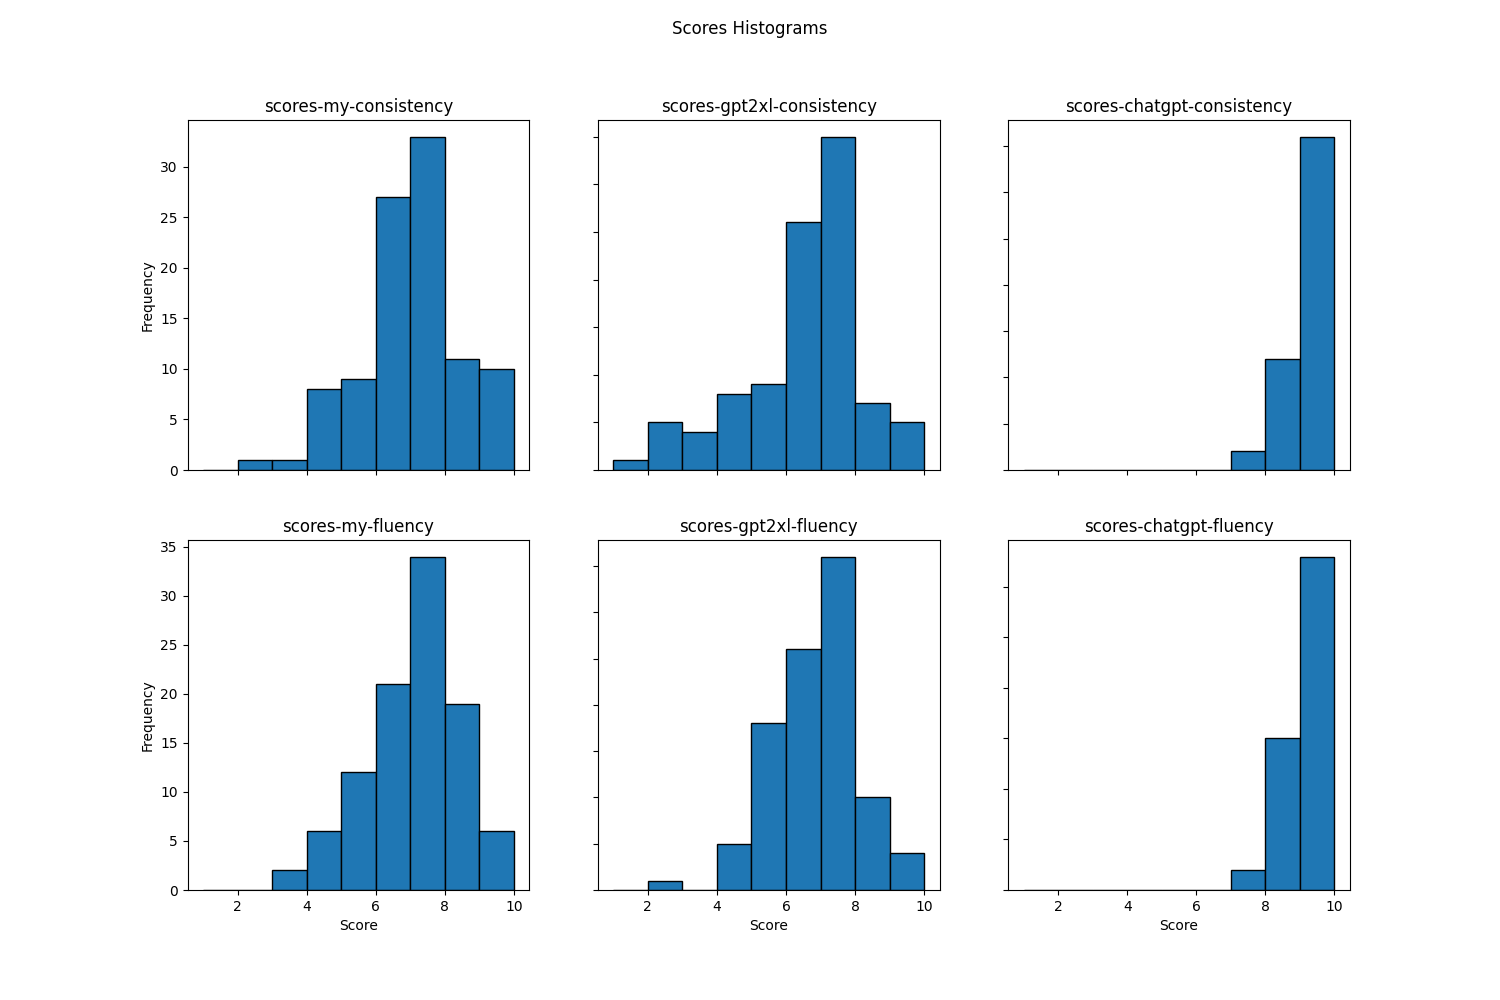
\includegraphics[width=500pt]{bar-hists.png}

\textbf{Average scores-my-consistency score: 6.53}\\
\textbf{Average scores-my-fluency score: 6.6}\\
\textbf{Average scores-gpt2xl-consistency score: 6.02}\\
\textbf{Average scores-gpt2xl-fluency score: 6.36}\\
\textbf{Average scores-chatgpt-consistency score: 8.79}\\
\textbf{Average scores-chatgpt-fluency score: 8.66}\\

\textbf{\large My model definitely outperforms GPT2-XL.}


\end{document}

